\documentclass[twoside]{book}

% Packages required by doxygen
\usepackage{fixltx2e}
\usepackage{calc}
\usepackage{doxygen}
\usepackage[export]{adjustbox} % also loads graphicx
\usepackage{graphicx}
\usepackage[utf8]{inputenc}
\usepackage{makeidx}
\usepackage{multicol}
\usepackage{multirow}
\PassOptionsToPackage{warn}{textcomp}
\usepackage{textcomp}
\usepackage[nointegrals]{wasysym}
\usepackage[table]{xcolor}

% Font selection
\usepackage[T1]{fontenc}
\usepackage[scaled=.90]{helvet}
\usepackage{courier}
\usepackage{amssymb}
\usepackage{sectsty}
\renewcommand{\familydefault}{\sfdefault}
\allsectionsfont{%
  \fontseries{bc}\selectfont%
  \color{darkgray}%
}
\renewcommand{\DoxyLabelFont}{%
  \fontseries{bc}\selectfont%
  \color{darkgray}%
}
\newcommand{\+}{\discretionary{\mbox{\scriptsize$\hookleftarrow$}}{}{}}

% Page & text layout
\usepackage{geometry}
\geometry{%
  a4paper,%
  top=2.5cm,%
  bottom=2.5cm,%
  left=2.5cm,%
  right=2.5cm%
}
\tolerance=750
\hfuzz=15pt
\hbadness=750
\setlength{\emergencystretch}{15pt}
\setlength{\parindent}{0cm}
\setlength{\parskip}{3ex plus 2ex minus 2ex}
\makeatletter
\renewcommand{\paragraph}{%
  \@startsection{paragraph}{4}{0ex}{-1.0ex}{1.0ex}{%
    \normalfont\normalsize\bfseries\SS@parafont%
  }%
}
\renewcommand{\subparagraph}{%
  \@startsection{subparagraph}{5}{0ex}{-1.0ex}{1.0ex}{%
    \normalfont\normalsize\bfseries\SS@subparafont%
  }%
}
\makeatother

% Headers & footers
\usepackage{fancyhdr}
\pagestyle{fancyplain}
\fancyhead[LE]{\fancyplain{}{\bfseries\thepage}}
\fancyhead[CE]{\fancyplain{}{}}
\fancyhead[RE]{\fancyplain{}{\bfseries\leftmark}}
\fancyhead[LO]{\fancyplain{}{\bfseries\rightmark}}
\fancyhead[CO]{\fancyplain{}{}}
\fancyhead[RO]{\fancyplain{}{\bfseries\thepage}}
\fancyfoot[LE]{\fancyplain{}{}}
\fancyfoot[CE]{\fancyplain{}{}}
\fancyfoot[RE]{\fancyplain{}{\bfseries\scriptsize Generated by Doxygen }}
\fancyfoot[LO]{\fancyplain{}{\bfseries\scriptsize Generated by Doxygen }}
\fancyfoot[CO]{\fancyplain{}{}}
\fancyfoot[RO]{\fancyplain{}{}}
\renewcommand{\footrulewidth}{0.4pt}
\renewcommand{\chaptermark}[1]{%
  \markboth{#1}{}%
}
\renewcommand{\sectionmark}[1]{%
  \markright{\thesection\ #1}%
}

% Indices & bibliography
\usepackage{natbib}
\usepackage[titles]{tocloft}
\setcounter{tocdepth}{3}
\setcounter{secnumdepth}{5}
\makeindex

% Hyperlinks (required, but should be loaded last)
\usepackage{ifpdf}
\ifpdf
  \usepackage[pdftex,pagebackref=true]{hyperref}
\else
  \usepackage[ps2pdf,pagebackref=true]{hyperref}
\fi
\hypersetup{%
  colorlinks=true,%
  linkcolor=blue,%
  citecolor=blue,%
  unicode%
}

% Custom commands
\newcommand{\clearemptydoublepage}{%
  \newpage{\pagestyle{empty}\cleardoublepage}%
}

\usepackage{caption}
\captionsetup{labelsep=space,justification=centering,font={bf},singlelinecheck=off,skip=4pt,position=top}

%===== C O N T E N T S =====

\begin{document}

% Titlepage & ToC
\hypersetup{pageanchor=false,
             bookmarksnumbered=true,
             pdfencoding=unicode
            }
\pagenumbering{alph}
\begin{titlepage}
\vspace*{7cm}
\begin{center}%
{\Large B\+A\+B\+E\+L\+\_\+\+N\+U\+M\+B\+ER }\\
\vspace*{1cm}
{\large Generated by Doxygen 1.8.14}\\
\end{center}
\end{titlepage}
\clearemptydoublepage
\pagenumbering{roman}
\tableofcontents
\clearemptydoublepage
\pagenumbering{arabic}
\hypersetup{pageanchor=true}

%--- Begin generated contents ---
\chapter{Hierarchical Index}
\section{Class Hierarchy}
This inheritance list is sorted roughly, but not completely, alphabetically\+:\begin{DoxyCompactList}
\item \contentsline{section}{Audio\+Compressor}{\pageref{classAudioCompressor}}{}
\item \contentsline{section}{Audio\+Packet}{\pageref{structAudioPacket}}{}
\item exception\begin{DoxyCompactList}
\item \contentsline{section}{Audio\+Exception}{\pageref{classAudioException}}{}
\end{DoxyCompactList}
\item \contentsline{section}{Packet}{\pageref{structPacket}}{}
\item Q\+Main\+Window\begin{DoxyCompactList}
\item \contentsline{section}{Main\+Window}{\pageref{classMainWindow}}{}
\end{DoxyCompactList}
\item Q\+Object\begin{DoxyCompactList}
\item \contentsline{section}{Audio\+Wrapper}{\pageref{classAudioWrapper}}{}
\item \contentsline{section}{Tcp\+Client}{\pageref{classTcpClient}}{}
\item \contentsline{section}{Udp\+Client}{\pageref{classUdpClient}}{}
\end{DoxyCompactList}
\item \contentsline{section}{Ui\+\_\+\+Main\+Window}{\pageref{classUi__MainWindow}}{}
\begin{DoxyCompactList}
\item \contentsline{section}{Ui\+:\+:Main\+Window}{\pageref{classUi_1_1MainWindow}}{}
\end{DoxyCompactList}
\end{DoxyCompactList}

\chapter{Class Index}
\section{Class List}
Here are the classes, structs, unions and interfaces with brief descriptions\+:\begin{DoxyCompactList}
\item\contentsline{section}{\mbox{\hyperlink{classAudioCompressor}{Audio\+Compressor}} }{\pageref{classAudioCompressor}}{}
\item\contentsline{section}{\mbox{\hyperlink{classAudioException}{Audio\+Exception}} }{\pageref{classAudioException}}{}
\item\contentsline{section}{\mbox{\hyperlink{structAudioPacket}{Audio\+Packet}} }{\pageref{structAudioPacket}}{}
\item\contentsline{section}{\mbox{\hyperlink{classAudioWrapper}{Audio\+Wrapper}} }{\pageref{classAudioWrapper}}{}
\item\contentsline{section}{\mbox{\hyperlink{classMainWindow}{Main\+Window}} }{\pageref{classMainWindow}}{}
\item\contentsline{section}{\mbox{\hyperlink{classUi_1_1MainWindow}{Ui\+::\+Main\+Window}} }{\pageref{classUi_1_1MainWindow}}{}
\item\contentsline{section}{\mbox{\hyperlink{structPacket}{Packet}} }{\pageref{structPacket}}{}
\item\contentsline{section}{\mbox{\hyperlink{classTcpClient}{Tcp\+Client}} }{\pageref{classTcpClient}}{}
\item\contentsline{section}{\mbox{\hyperlink{classUdpClient}{Udp\+Client}} }{\pageref{classUdpClient}}{}
\item\contentsline{section}{\mbox{\hyperlink{classUi__MainWindow}{Ui\+\_\+\+Main\+Window}} }{\pageref{classUi__MainWindow}}{}
\end{DoxyCompactList}

\chapter{File Index}
\section{File List}
Here is a list of all files with brief descriptions\+:\begin{DoxyCompactList}
\item\contentsline{section}{\mbox{\hyperlink{main_8cpp}{main.\+cpp}} }{\pageref{main_8cpp}}{}
\item\contentsline{section}{database/\mbox{\hyperlink{IDataBaseProvider_8hpp}{I\+Data\+Base\+Provider.\+hpp}} }{\pageref{IDataBaseProvider_8hpp}}{}
\item\contentsline{section}{database/\mbox{\hyperlink{SqliteProvider_8cpp}{Sqlite\+Provider.\+cpp}} }{\pageref{SqliteProvider_8cpp}}{}
\item\contentsline{section}{database/\mbox{\hyperlink{SqliteProvider_8hpp}{Sqlite\+Provider.\+hpp}} }{\pageref{SqliteProvider_8hpp}}{}
\item\contentsline{section}{logic/\mbox{\hyperlink{Client_8hpp}{Client.\+hpp}} }{\pageref{Client_8hpp}}{}
\item\contentsline{section}{logic/handshake/\mbox{\hyperlink{HandshakeHandler_8cpp}{Handshake\+Handler.\+cpp}} }{\pageref{HandshakeHandler_8cpp}}{}
\item\contentsline{section}{logic/handshake/\mbox{\hyperlink{HandshakeHandler_8hpp}{Handshake\+Handler.\+hpp}} }{\pageref{HandshakeHandler_8hpp}}{}
\item\contentsline{section}{network/\mbox{\hyperlink{BoostConnection_8cpp}{Boost\+Connection.\+cpp}} }{\pageref{BoostConnection_8cpp}}{}
\item\contentsline{section}{network/\mbox{\hyperlink{BoostConnection_8hpp}{Boost\+Connection.\+hpp}} }{\pageref{BoostConnection_8hpp}}{}
\item\contentsline{section}{network/\mbox{\hyperlink{BoostListener_8cpp}{Boost\+Listener.\+cpp}} }{\pageref{BoostListener_8cpp}}{}
\item\contentsline{section}{network/\mbox{\hyperlink{BoostListener_8hpp}{Boost\+Listener.\+hpp}} }{\pageref{BoostListener_8hpp}}{}
\item\contentsline{section}{network/\mbox{\hyperlink{IConnection_8hpp}{I\+Connection.\+hpp}} }{\pageref{IConnection_8hpp}}{}
\item\contentsline{section}{network/\mbox{\hyperlink{IListener_8hpp}{I\+Listener.\+hpp}} }{\pageref{IListener_8hpp}}{}
\item\contentsline{section}{queue/\mbox{\hyperlink{ConcurrentQueue_8hpp}{Concurrent\+Queue.\+hpp}} }{\pageref{ConcurrentQueue_8hpp}}{}
\item\contentsline{section}{services/\mbox{\hyperlink{BoostService_8hpp}{Boost\+Service.\+hpp}} }{\pageref{BoostService_8hpp}}{}
\item\contentsline{section}{services/\mbox{\hyperlink{DataBaseService_8hpp}{Data\+Base\+Service.\+hpp}} }{\pageref{DataBaseService_8hpp}}{}
\item\contentsline{section}{services/\mbox{\hyperlink{DispatchService_8hpp}{Dispatch\+Service.\+hpp}} }{\pageref{DispatchService_8hpp}}{}
\item\contentsline{section}{services/\mbox{\hyperlink{HandlerService_8cpp}{Handler\+Service.\+cpp}} }{\pageref{HandlerService_8cpp}}{}
\item\contentsline{section}{services/\mbox{\hyperlink{HandlerService_8hpp}{Handler\+Service.\+hpp}} }{\pageref{HandlerService_8hpp}}{}
\item\contentsline{section}{services/\mbox{\hyperlink{IService_8hpp}{I\+Service.\+hpp}} }{\pageref{IService_8hpp}}{}
\item\contentsline{section}{services/\mbox{\hyperlink{LogService_8hpp}{Log\+Service.\+hpp}} }{\pageref{LogService_8hpp}}{}
\item\contentsline{section}{services/\mbox{\hyperlink{NetworkService_8hpp}{Network\+Service.\+hpp}} }{\pageref{NetworkService_8hpp}}{}
\item\contentsline{section}{services/\mbox{\hyperlink{ServiceLocator_8hpp}{Service\+Locator.\+hpp}} }{\pageref{ServiceLocator_8hpp}}{}
\item\contentsline{section}{services/\mbox{\hyperlink{UserService_8hpp}{User\+Service.\+hpp}} }{\pageref{UserService_8hpp}}{}
\end{DoxyCompactList}

\chapter{Class Documentation}
\hypertarget{classBoostConnection}{}\section{Boost\+Connection Class Reference}
\label{classBoostConnection}\index{Boost\+Connection@{Boost\+Connection}}


{\ttfamily \#include $<$Boost\+Connection.\+hpp$>$}



Inheritance diagram for Boost\+Connection\+:
\nopagebreak
\begin{figure}[H]
\begin{center}
\leavevmode
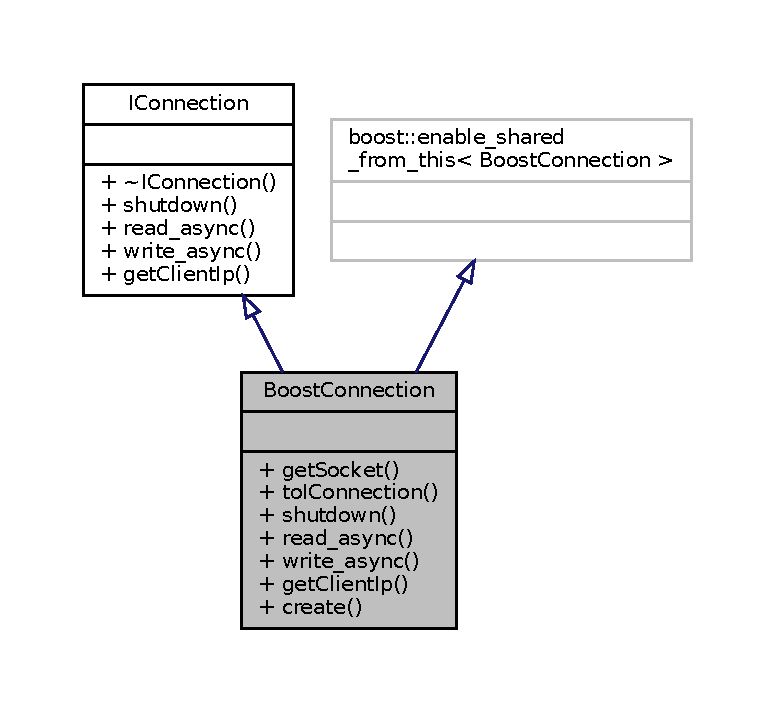
\includegraphics[width=350pt]{classBoostConnection__inherit__graph}
\end{center}
\end{figure}


Collaboration diagram for Boost\+Connection\+:
\nopagebreak
\begin{figure}[H]
\begin{center}
\leavevmode
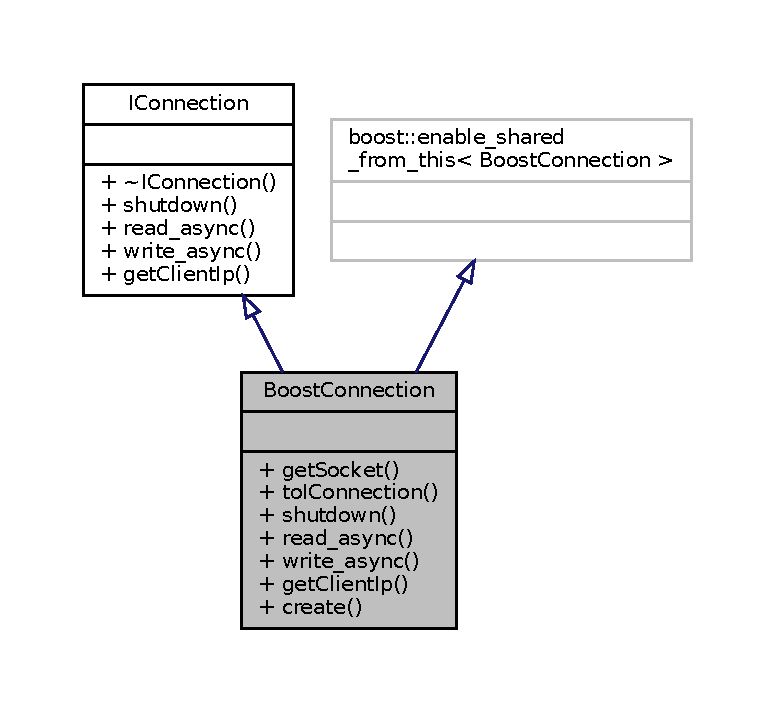
\includegraphics[width=350pt]{classBoostConnection__coll__graph}
\end{center}
\end{figure}
\subsection*{Public Types}
\begin{DoxyCompactItemize}
\item 
using \mbox{\hyperlink{classBoostConnection_acaf86877128a2df13130110cf72de640}{pointer}} = boost\+::shared\+\_\+ptr$<$ \mbox{\hyperlink{classBoostConnection}{Boost\+Connection}} $>$
\end{DoxyCompactItemize}
\subsection*{Public Member Functions}
\begin{DoxyCompactItemize}
\item 
boost\+::asio\+::ip\+::tcp\+::socket \& \mbox{\hyperlink{classBoostConnection_a5b83b6847a7a522439fb6f66fd11b9e5}{get\+Socket}} ()
\item 
boost\+::shared\+\_\+ptr$<$ \mbox{\hyperlink{classIConnection}{I\+Connection}} $>$ \mbox{\hyperlink{classBoostConnection_a3262569e07575555bff604a7f9f6c803}{to\+I\+Connection}} ()
\item 
void \mbox{\hyperlink{classBoostConnection_a576ca28ef2f8f335ee1a0ccab64cc55b}{shutdown}} () override
\item 
void \mbox{\hyperlink{classBoostConnection_a8b117337238e2652adecde8971c1ab93}{read\+\_\+async}} () override
\item 
void \mbox{\hyperlink{classBoostConnection_abe7200e60f8b4d909a057f85ca9569db}{write\+\_\+async}} (const std\+::string \&message) override
\item 
std\+::string \mbox{\hyperlink{classBoostConnection_a648ba5a8674fc95b4cab8c94225a19e9}{get\+Client\+Ip}} () const override
\end{DoxyCompactItemize}
\subsection*{Static Public Member Functions}
\begin{DoxyCompactItemize}
\item 
static \mbox{\hyperlink{classBoostConnection_acaf86877128a2df13130110cf72de640}{pointer}} \mbox{\hyperlink{classBoostConnection_a2f020a5317924e126c1495a86816f8ef}{create}} ()
\end{DoxyCompactItemize}


\subsection{Member Typedef Documentation}
\mbox{\Hypertarget{classBoostConnection_acaf86877128a2df13130110cf72de640}\label{classBoostConnection_acaf86877128a2df13130110cf72de640}} 
\index{Boost\+Connection@{Boost\+Connection}!pointer@{pointer}}
\index{pointer@{pointer}!Boost\+Connection@{Boost\+Connection}}
\subsubsection{\texorpdfstring{pointer}{pointer}}
{\footnotesize\ttfamily using \mbox{\hyperlink{classBoostConnection_acaf86877128a2df13130110cf72de640}{Boost\+Connection\+::pointer}} =  boost\+::shared\+\_\+ptr$<$\mbox{\hyperlink{classBoostConnection}{Boost\+Connection}}$>$}



\subsection{Member Function Documentation}
\mbox{\Hypertarget{classBoostConnection_a2f020a5317924e126c1495a86816f8ef}\label{classBoostConnection_a2f020a5317924e126c1495a86816f8ef}} 
\index{Boost\+Connection@{Boost\+Connection}!create@{create}}
\index{create@{create}!Boost\+Connection@{Boost\+Connection}}
\subsubsection{\texorpdfstring{create()}{create()}}
{\footnotesize\ttfamily static \mbox{\hyperlink{classBoostConnection_acaf86877128a2df13130110cf72de640}{pointer}} Boost\+Connection\+::create (\begin{DoxyParamCaption}{ }\end{DoxyParamCaption})\hspace{0.3cm}{\ttfamily [inline]}, {\ttfamily [static]}}

\mbox{\Hypertarget{classBoostConnection_a648ba5a8674fc95b4cab8c94225a19e9}\label{classBoostConnection_a648ba5a8674fc95b4cab8c94225a19e9}} 
\index{Boost\+Connection@{Boost\+Connection}!get\+Client\+Ip@{get\+Client\+Ip}}
\index{get\+Client\+Ip@{get\+Client\+Ip}!Boost\+Connection@{Boost\+Connection}}
\subsubsection{\texorpdfstring{get\+Client\+Ip()}{getClientIp()}}
{\footnotesize\ttfamily std\+::string Boost\+Connection\+::get\+Client\+Ip (\begin{DoxyParamCaption}{ }\end{DoxyParamCaption}) const\hspace{0.3cm}{\ttfamily [override]}, {\ttfamily [virtual]}}



Implements \mbox{\hyperlink{classIConnection_a7064757e5c427496f482239dde7e0540}{I\+Connection}}.

\mbox{\Hypertarget{classBoostConnection_a5b83b6847a7a522439fb6f66fd11b9e5}\label{classBoostConnection_a5b83b6847a7a522439fb6f66fd11b9e5}} 
\index{Boost\+Connection@{Boost\+Connection}!get\+Socket@{get\+Socket}}
\index{get\+Socket@{get\+Socket}!Boost\+Connection@{Boost\+Connection}}
\subsubsection{\texorpdfstring{get\+Socket()}{getSocket()}}
{\footnotesize\ttfamily boost\+::asio\+::ip\+::tcp\+::socket\& Boost\+Connection\+::get\+Socket (\begin{DoxyParamCaption}{ }\end{DoxyParamCaption})\hspace{0.3cm}{\ttfamily [inline]}}

\mbox{\Hypertarget{classBoostConnection_a8b117337238e2652adecde8971c1ab93}\label{classBoostConnection_a8b117337238e2652adecde8971c1ab93}} 
\index{Boost\+Connection@{Boost\+Connection}!read\+\_\+async@{read\+\_\+async}}
\index{read\+\_\+async@{read\+\_\+async}!Boost\+Connection@{Boost\+Connection}}
\subsubsection{\texorpdfstring{read\+\_\+async()}{read\_async()}}
{\footnotesize\ttfamily void Boost\+Connection\+::read\+\_\+async (\begin{DoxyParamCaption}{ }\end{DoxyParamCaption})\hspace{0.3cm}{\ttfamily [override]}, {\ttfamily [virtual]}}



Implements \mbox{\hyperlink{classIConnection_a1c9d492241a79546f243088285279144}{I\+Connection}}.

\mbox{\Hypertarget{classBoostConnection_a576ca28ef2f8f335ee1a0ccab64cc55b}\label{classBoostConnection_a576ca28ef2f8f335ee1a0ccab64cc55b}} 
\index{Boost\+Connection@{Boost\+Connection}!shutdown@{shutdown}}
\index{shutdown@{shutdown}!Boost\+Connection@{Boost\+Connection}}
\subsubsection{\texorpdfstring{shutdown()}{shutdown()}}
{\footnotesize\ttfamily void Boost\+Connection\+::shutdown (\begin{DoxyParamCaption}{ }\end{DoxyParamCaption})\hspace{0.3cm}{\ttfamily [override]}, {\ttfamily [virtual]}}



Implements \mbox{\hyperlink{classIConnection_ae15b6922f3a31a7f316a6390eb2469b2}{I\+Connection}}.

\mbox{\Hypertarget{classBoostConnection_a3262569e07575555bff604a7f9f6c803}\label{classBoostConnection_a3262569e07575555bff604a7f9f6c803}} 
\index{Boost\+Connection@{Boost\+Connection}!to\+I\+Connection@{to\+I\+Connection}}
\index{to\+I\+Connection@{to\+I\+Connection}!Boost\+Connection@{Boost\+Connection}}
\subsubsection{\texorpdfstring{to\+I\+Connection()}{toIConnection()}}
{\footnotesize\ttfamily boost\+::shared\+\_\+ptr$<$\mbox{\hyperlink{classIConnection}{I\+Connection}}$>$ Boost\+Connection\+::to\+I\+Connection (\begin{DoxyParamCaption}{ }\end{DoxyParamCaption})\hspace{0.3cm}{\ttfamily [inline]}}

\mbox{\Hypertarget{classBoostConnection_abe7200e60f8b4d909a057f85ca9569db}\label{classBoostConnection_abe7200e60f8b4d909a057f85ca9569db}} 
\index{Boost\+Connection@{Boost\+Connection}!write\+\_\+async@{write\+\_\+async}}
\index{write\+\_\+async@{write\+\_\+async}!Boost\+Connection@{Boost\+Connection}}
\subsubsection{\texorpdfstring{write\+\_\+async()}{write\_async()}}
{\footnotesize\ttfamily void Boost\+Connection\+::write\+\_\+async (\begin{DoxyParamCaption}\item[{const std\+::string \&}]{message }\end{DoxyParamCaption})\hspace{0.3cm}{\ttfamily [override]}, {\ttfamily [virtual]}}



Implements \mbox{\hyperlink{classIConnection_a7210f770ebae6277e98142a8b5a6226f}{I\+Connection}}.



The documentation for this class was generated from the following files\+:\begin{DoxyCompactItemize}
\item 
network/\mbox{\hyperlink{BoostConnection_8hpp}{Boost\+Connection.\+hpp}}\item 
network/\mbox{\hyperlink{BoostConnection_8cpp}{Boost\+Connection.\+cpp}}\end{DoxyCompactItemize}

\hypertarget{classBoostListener}{}\section{Boost\+Listener Class Reference}
\label{classBoostListener}\index{Boost\+Listener@{Boost\+Listener}}


{\ttfamily \#include $<$Boost\+Listener.\+hpp$>$}



Inheritance diagram for Boost\+Listener\+:
\nopagebreak
\begin{figure}[H]
\begin{center}
\leavevmode
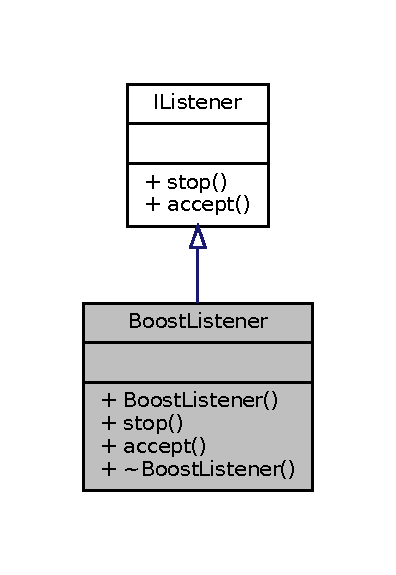
\includegraphics[width=190pt]{classBoostListener__inherit__graph}
\end{center}
\end{figure}


Collaboration diagram for Boost\+Listener\+:
\nopagebreak
\begin{figure}[H]
\begin{center}
\leavevmode
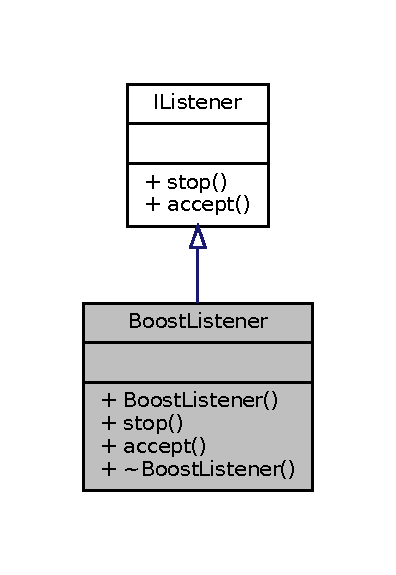
\includegraphics[width=190pt]{classBoostListener__coll__graph}
\end{center}
\end{figure}
\subsection*{Public Member Functions}
\begin{DoxyCompactItemize}
\item 
\mbox{\hyperlink{classBoostListener_a027dfad49bde876bf71ce8a27a437ac9}{Boost\+Listener}} (int port=\mbox{\hyperlink{IListener_8hpp_ae15716c4b5a51141b4029e52c2c2a744}{L\+I\+S\+T\+E\+N\+E\+R\+\_\+\+D\+E\+F\+A\+U\+L\+T\+\_\+\+P\+O\+RT}})
\item 
void \mbox{\hyperlink{classBoostListener_af83620fe2b6644903a6f631b8df2fd2d}{stop}} () override
\item 
void \mbox{\hyperlink{classBoostListener_a8a2849f0e1c513750bc74cb9a2c0d428}{accept}} () override
\item 
\mbox{\hyperlink{classBoostListener_ad50826b92d445b7e101ca261741b43b1}{$\sim$\+Boost\+Listener}} ()
\end{DoxyCompactItemize}


\subsection{Constructor \& Destructor Documentation}
\mbox{\Hypertarget{classBoostListener_a027dfad49bde876bf71ce8a27a437ac9}\label{classBoostListener_a027dfad49bde876bf71ce8a27a437ac9}} 
\index{Boost\+Listener@{Boost\+Listener}!Boost\+Listener@{Boost\+Listener}}
\index{Boost\+Listener@{Boost\+Listener}!Boost\+Listener@{Boost\+Listener}}
\subsubsection{\texorpdfstring{Boost\+Listener()}{BoostListener()}}
{\footnotesize\ttfamily Boost\+Listener\+::\+Boost\+Listener (\begin{DoxyParamCaption}\item[{int}]{port = {\ttfamily \mbox{\hyperlink{IListener_8hpp_ae15716c4b5a51141b4029e52c2c2a744}{L\+I\+S\+T\+E\+N\+E\+R\+\_\+\+D\+E\+F\+A\+U\+L\+T\+\_\+\+P\+O\+RT}}} }\end{DoxyParamCaption})\hspace{0.3cm}{\ttfamily [inline]}, {\ttfamily [explicit]}}

\mbox{\Hypertarget{classBoostListener_ad50826b92d445b7e101ca261741b43b1}\label{classBoostListener_ad50826b92d445b7e101ca261741b43b1}} 
\index{Boost\+Listener@{Boost\+Listener}!````~Boost\+Listener@{$\sim$\+Boost\+Listener}}
\index{````~Boost\+Listener@{$\sim$\+Boost\+Listener}!Boost\+Listener@{Boost\+Listener}}
\subsubsection{\texorpdfstring{$\sim$\+Boost\+Listener()}{~BoostListener()}}
{\footnotesize\ttfamily Boost\+Listener\+::$\sim$\+Boost\+Listener (\begin{DoxyParamCaption}{ }\end{DoxyParamCaption})\hspace{0.3cm}{\ttfamily [inline]}}

Here is the call graph for this function\+:
\nopagebreak
\begin{figure}[H]
\begin{center}
\leavevmode
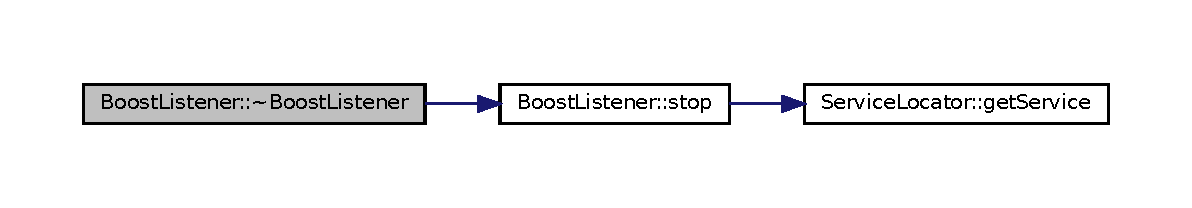
\includegraphics[width=350pt]{classBoostListener_ad50826b92d445b7e101ca261741b43b1_cgraph}
\end{center}
\end{figure}


\subsection{Member Function Documentation}
\mbox{\Hypertarget{classBoostListener_a8a2849f0e1c513750bc74cb9a2c0d428}\label{classBoostListener_a8a2849f0e1c513750bc74cb9a2c0d428}} 
\index{Boost\+Listener@{Boost\+Listener}!accept@{accept}}
\index{accept@{accept}!Boost\+Listener@{Boost\+Listener}}
\subsubsection{\texorpdfstring{accept()}{accept()}}
{\footnotesize\ttfamily void Boost\+Listener\+::accept (\begin{DoxyParamCaption}{ }\end{DoxyParamCaption})\hspace{0.3cm}{\ttfamily [override]}, {\ttfamily [virtual]}}



Implements \mbox{\hyperlink{classIListener_a332f291fb10f7dadc223fe6c9a98a7cc}{I\+Listener}}.

Here is the call graph for this function\+:
\nopagebreak
\begin{figure}[H]
\begin{center}
\leavevmode
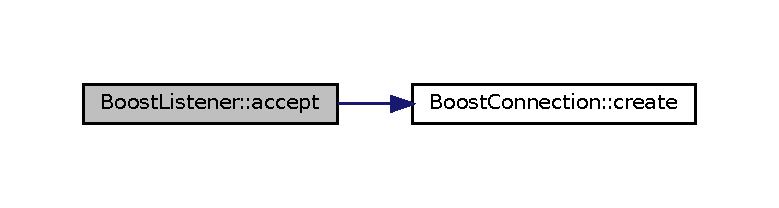
\includegraphics[width=350pt]{classBoostListener_a8a2849f0e1c513750bc74cb9a2c0d428_cgraph}
\end{center}
\end{figure}
\mbox{\Hypertarget{classBoostListener_af83620fe2b6644903a6f631b8df2fd2d}\label{classBoostListener_af83620fe2b6644903a6f631b8df2fd2d}} 
\index{Boost\+Listener@{Boost\+Listener}!stop@{stop}}
\index{stop@{stop}!Boost\+Listener@{Boost\+Listener}}
\subsubsection{\texorpdfstring{stop()}{stop()}}
{\footnotesize\ttfamily void Boost\+Listener\+::stop (\begin{DoxyParamCaption}{ }\end{DoxyParamCaption})\hspace{0.3cm}{\ttfamily [override]}, {\ttfamily [virtual]}}



Implements \mbox{\hyperlink{classIListener_a288f3ad930bc90086f4e8b6578609366}{I\+Listener}}.

Here is the call graph for this function\+:
\nopagebreak
\begin{figure}[H]
\begin{center}
\leavevmode
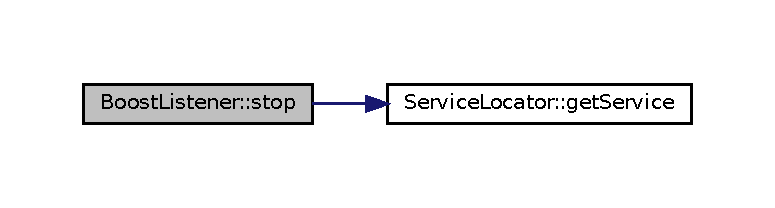
\includegraphics[width=350pt]{classBoostListener_af83620fe2b6644903a6f631b8df2fd2d_cgraph}
\end{center}
\end{figure}


The documentation for this class was generated from the following files\+:\begin{DoxyCompactItemize}
\item 
network/\mbox{\hyperlink{BoostListener_8hpp}{Boost\+Listener.\+hpp}}\item 
network/\mbox{\hyperlink{BoostListener_8cpp}{Boost\+Listener.\+cpp}}\end{DoxyCompactItemize}

\hypertarget{classBoostService}{}\section{Boost\+Service Class Reference}
\label{classBoostService}\index{Boost\+Service@{Boost\+Service}}


{\ttfamily \#include $<$Boost\+Service.\+hpp$>$}



Inheritance diagram for Boost\+Service\+:
\nopagebreak
\begin{figure}[H]
\begin{center}
\leavevmode
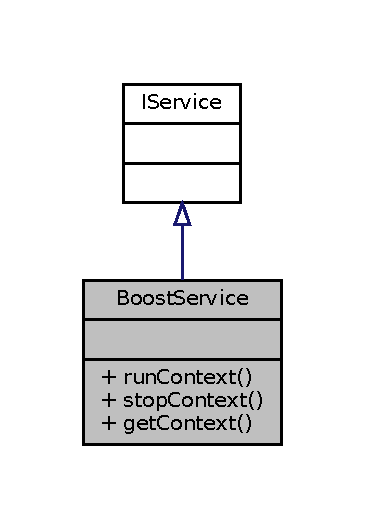
\includegraphics[width=175pt]{classBoostService__inherit__graph}
\end{center}
\end{figure}


Collaboration diagram for Boost\+Service\+:
\nopagebreak
\begin{figure}[H]
\begin{center}
\leavevmode
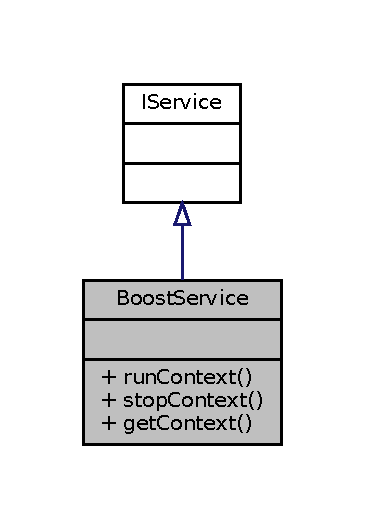
\includegraphics[width=175pt]{classBoostService__coll__graph}
\end{center}
\end{figure}
\subsection*{Public Member Functions}
\begin{DoxyCompactItemize}
\item 
void const \mbox{\hyperlink{classBoostService_a6a8766ff5a3c5ff42c9c114395d50565}{run\+Context}} ()
\item 
void const \mbox{\hyperlink{classBoostService_aff4e11e835ba4961f30f51c7bfa6be6e}{stop\+Context}} ()
\item 
boost\+::asio\+::io\+\_\+context \& \mbox{\hyperlink{classBoostService_ad5fab5bcc9c64c1b2c4b8fcf4b005b1a}{get\+Context}} ()
\end{DoxyCompactItemize}


\subsection{Member Function Documentation}
\mbox{\Hypertarget{classBoostService_ad5fab5bcc9c64c1b2c4b8fcf4b005b1a}\label{classBoostService_ad5fab5bcc9c64c1b2c4b8fcf4b005b1a}} 
\index{Boost\+Service@{Boost\+Service}!get\+Context@{get\+Context}}
\index{get\+Context@{get\+Context}!Boost\+Service@{Boost\+Service}}
\subsubsection{\texorpdfstring{get\+Context()}{getContext()}}
{\footnotesize\ttfamily boost\+::asio\+::io\+\_\+context\& Boost\+Service\+::get\+Context (\begin{DoxyParamCaption}{ }\end{DoxyParamCaption})\hspace{0.3cm}{\ttfamily [inline]}}

\mbox{\Hypertarget{classBoostService_a6a8766ff5a3c5ff42c9c114395d50565}\label{classBoostService_a6a8766ff5a3c5ff42c9c114395d50565}} 
\index{Boost\+Service@{Boost\+Service}!run\+Context@{run\+Context}}
\index{run\+Context@{run\+Context}!Boost\+Service@{Boost\+Service}}
\subsubsection{\texorpdfstring{run\+Context()}{runContext()}}
{\footnotesize\ttfamily void const Boost\+Service\+::run\+Context (\begin{DoxyParamCaption}{ }\end{DoxyParamCaption})\hspace{0.3cm}{\ttfamily [inline]}}

\mbox{\Hypertarget{classBoostService_aff4e11e835ba4961f30f51c7bfa6be6e}\label{classBoostService_aff4e11e835ba4961f30f51c7bfa6be6e}} 
\index{Boost\+Service@{Boost\+Service}!stop\+Context@{stop\+Context}}
\index{stop\+Context@{stop\+Context}!Boost\+Service@{Boost\+Service}}
\subsubsection{\texorpdfstring{stop\+Context()}{stopContext()}}
{\footnotesize\ttfamily void const Boost\+Service\+::stop\+Context (\begin{DoxyParamCaption}{ }\end{DoxyParamCaption})\hspace{0.3cm}{\ttfamily [inline]}}



The documentation for this class was generated from the following file\+:\begin{DoxyCompactItemize}
\item 
services/\mbox{\hyperlink{BoostService_8hpp}{Boost\+Service.\+hpp}}\end{DoxyCompactItemize}

\hypertarget{classClient}{}\section{Client Class Reference}
\label{classClient}\index{Client@{Client}}


{\ttfamily \#include $<$Client.\+hpp$>$}



Collaboration diagram for Client\+:
\nopagebreak
\begin{figure}[H]
\begin{center}
\leavevmode
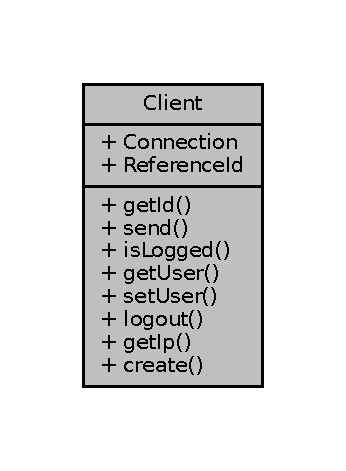
\includegraphics[width=166pt]{classClient__coll__graph}
\end{center}
\end{figure}
\subsection*{Public Member Functions}
\begin{DoxyCompactItemize}
\item 
int \mbox{\hyperlink{classClient_abc4d8d86cc753596a08a90e359f5eb31}{get\+Id}} ()
\item 
void \mbox{\hyperlink{classClient_ab26edfd53bf1deeab0aac1715858f279}{send}} (const I\+Packet \&packet)
\item 
bool \mbox{\hyperlink{classClient_afcbe6046c74e86b64c1b861f5e58ffbd}{is\+Logged}} () const
\item 
const \mbox{\hyperlink{structUser}{User}} \& \mbox{\hyperlink{classClient_a31da08b532d6585e61d98b563177e33a}{get\+User}} () const
\item 
void \mbox{\hyperlink{classClient_a902b85e55694c497acf50deb082cb23e}{set\+User}} (const \mbox{\hyperlink{structUser}{User}} \&user)
\item 
void \mbox{\hyperlink{classClient_aa977795294407c10fe843b5bc28b6685}{logout}} ()
\item 
std\+::string \mbox{\hyperlink{classClient_ab04ab042f49fd43a6eaeb8df05eb0eae}{get\+Ip}} () const
\end{DoxyCompactItemize}
\subsection*{Static Public Member Functions}
\begin{DoxyCompactItemize}
\item 
static boost\+::shared\+\_\+ptr$<$ \mbox{\hyperlink{classClient}{Client}} $>$ \mbox{\hyperlink{classClient_a3d47022bf1a2f166fe04b80e9ec2bebc}{create}} (boost\+::shared\+\_\+ptr$<$ \mbox{\hyperlink{classIConnection}{I\+Connection}} $>$ \&connection)
\end{DoxyCompactItemize}
\subsection*{Public Attributes}
\begin{DoxyCompactItemize}
\item 
boost\+::shared\+\_\+ptr$<$ \mbox{\hyperlink{classIConnection}{I\+Connection}} $>$ \mbox{\hyperlink{classClient_acf0b64183e7b92d030224c3ae9b54655}{Connection}}
\end{DoxyCompactItemize}
\subsection*{Static Public Attributes}
\begin{DoxyCompactItemize}
\item 
static int \mbox{\hyperlink{classClient_a19fc58b997c5c69c2156a493983b0652}{Reference\+Id}} = 0
\end{DoxyCompactItemize}


\subsection{Member Function Documentation}
\mbox{\Hypertarget{classClient_a3d47022bf1a2f166fe04b80e9ec2bebc}\label{classClient_a3d47022bf1a2f166fe04b80e9ec2bebc}} 
\index{Client@{Client}!create@{create}}
\index{create@{create}!Client@{Client}}
\subsubsection{\texorpdfstring{create()}{create()}}
{\footnotesize\ttfamily static boost\+::shared\+\_\+ptr$<$\mbox{\hyperlink{classClient}{Client}}$>$ Client\+::create (\begin{DoxyParamCaption}\item[{boost\+::shared\+\_\+ptr$<$ \mbox{\hyperlink{classIConnection}{I\+Connection}} $>$ \&}]{connection }\end{DoxyParamCaption})\hspace{0.3cm}{\ttfamily [inline]}, {\ttfamily [static]}}

\mbox{\Hypertarget{classClient_abc4d8d86cc753596a08a90e359f5eb31}\label{classClient_abc4d8d86cc753596a08a90e359f5eb31}} 
\index{Client@{Client}!get\+Id@{get\+Id}}
\index{get\+Id@{get\+Id}!Client@{Client}}
\subsubsection{\texorpdfstring{get\+Id()}{getId()}}
{\footnotesize\ttfamily int Client\+::get\+Id (\begin{DoxyParamCaption}{ }\end{DoxyParamCaption})\hspace{0.3cm}{\ttfamily [inline]}}

\mbox{\Hypertarget{classClient_ab04ab042f49fd43a6eaeb8df05eb0eae}\label{classClient_ab04ab042f49fd43a6eaeb8df05eb0eae}} 
\index{Client@{Client}!get\+Ip@{get\+Ip}}
\index{get\+Ip@{get\+Ip}!Client@{Client}}
\subsubsection{\texorpdfstring{get\+Ip()}{getIp()}}
{\footnotesize\ttfamily std\+::string Client\+::get\+Ip (\begin{DoxyParamCaption}{ }\end{DoxyParamCaption}) const\hspace{0.3cm}{\ttfamily [inline]}}

\mbox{\Hypertarget{classClient_a31da08b532d6585e61d98b563177e33a}\label{classClient_a31da08b532d6585e61d98b563177e33a}} 
\index{Client@{Client}!get\+User@{get\+User}}
\index{get\+User@{get\+User}!Client@{Client}}
\subsubsection{\texorpdfstring{get\+User()}{getUser()}}
{\footnotesize\ttfamily const \mbox{\hyperlink{structUser}{User}}\& Client\+::get\+User (\begin{DoxyParamCaption}{ }\end{DoxyParamCaption}) const\hspace{0.3cm}{\ttfamily [inline]}}

Here is the call graph for this function\+:
\nopagebreak
\begin{figure}[H]
\begin{center}
\leavevmode
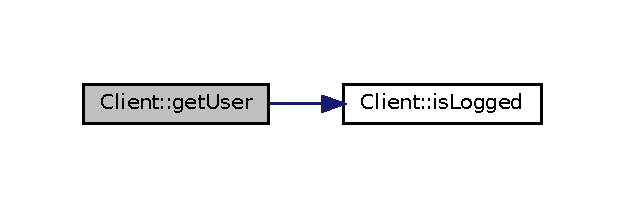
\includegraphics[width=300pt]{classClient_a31da08b532d6585e61d98b563177e33a_cgraph}
\end{center}
\end{figure}
\mbox{\Hypertarget{classClient_afcbe6046c74e86b64c1b861f5e58ffbd}\label{classClient_afcbe6046c74e86b64c1b861f5e58ffbd}} 
\index{Client@{Client}!is\+Logged@{is\+Logged}}
\index{is\+Logged@{is\+Logged}!Client@{Client}}
\subsubsection{\texorpdfstring{is\+Logged()}{isLogged()}}
{\footnotesize\ttfamily bool Client\+::is\+Logged (\begin{DoxyParamCaption}{ }\end{DoxyParamCaption}) const\hspace{0.3cm}{\ttfamily [inline]}}

\mbox{\Hypertarget{classClient_aa977795294407c10fe843b5bc28b6685}\label{classClient_aa977795294407c10fe843b5bc28b6685}} 
\index{Client@{Client}!logout@{logout}}
\index{logout@{logout}!Client@{Client}}
\subsubsection{\texorpdfstring{logout()}{logout()}}
{\footnotesize\ttfamily void Client\+::logout (\begin{DoxyParamCaption}{ }\end{DoxyParamCaption})\hspace{0.3cm}{\ttfamily [inline]}}

\mbox{\Hypertarget{classClient_ab26edfd53bf1deeab0aac1715858f279}\label{classClient_ab26edfd53bf1deeab0aac1715858f279}} 
\index{Client@{Client}!send@{send}}
\index{send@{send}!Client@{Client}}
\subsubsection{\texorpdfstring{send()}{send()}}
{\footnotesize\ttfamily void Client\+::send (\begin{DoxyParamCaption}\item[{const I\+Packet \&}]{packet }\end{DoxyParamCaption})\hspace{0.3cm}{\ttfamily [inline]}}

\mbox{\Hypertarget{classClient_a902b85e55694c497acf50deb082cb23e}\label{classClient_a902b85e55694c497acf50deb082cb23e}} 
\index{Client@{Client}!set\+User@{set\+User}}
\index{set\+User@{set\+User}!Client@{Client}}
\subsubsection{\texorpdfstring{set\+User()}{setUser()}}
{\footnotesize\ttfamily void Client\+::set\+User (\begin{DoxyParamCaption}\item[{const \mbox{\hyperlink{structUser}{User}} \&}]{user }\end{DoxyParamCaption})\hspace{0.3cm}{\ttfamily [inline]}}



\subsection{Member Data Documentation}
\mbox{\Hypertarget{classClient_acf0b64183e7b92d030224c3ae9b54655}\label{classClient_acf0b64183e7b92d030224c3ae9b54655}} 
\index{Client@{Client}!Connection@{Connection}}
\index{Connection@{Connection}!Client@{Client}}
\subsubsection{\texorpdfstring{Connection}{Connection}}
{\footnotesize\ttfamily boost\+::shared\+\_\+ptr$<$\mbox{\hyperlink{classIConnection}{I\+Connection}}$>$ Client\+::\+Connection}

\mbox{\Hypertarget{classClient_a19fc58b997c5c69c2156a493983b0652}\label{classClient_a19fc58b997c5c69c2156a493983b0652}} 
\index{Client@{Client}!Reference\+Id@{Reference\+Id}}
\index{Reference\+Id@{Reference\+Id}!Client@{Client}}
\subsubsection{\texorpdfstring{Reference\+Id}{ReferenceId}}
{\footnotesize\ttfamily int Client\+::\+Reference\+Id = 0\hspace{0.3cm}{\ttfamily [static]}}



The documentation for this class was generated from the following files\+:\begin{DoxyCompactItemize}
\item 
logic/\mbox{\hyperlink{Client_8hpp}{Client.\+hpp}}\item 
\mbox{\hyperlink{main_8cpp}{main.\+cpp}}\end{DoxyCompactItemize}

\hypertarget{classConcurrentQueue}{}\section{Concurrent\+Queue$<$ T $>$ Class Template Reference}
\label{classConcurrentQueue}\index{Concurrent\+Queue$<$ T $>$@{Concurrent\+Queue$<$ T $>$}}


{\ttfamily \#include $<$Concurrent\+Queue.\+hpp$>$}



Collaboration diagram for Concurrent\+Queue$<$ T $>$\+:
\nopagebreak
\begin{figure}[H]
\begin{center}
\leavevmode
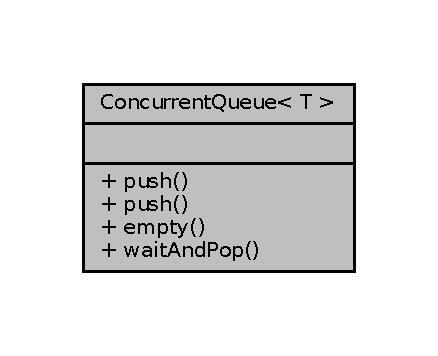
\includegraphics[width=210pt]{classConcurrentQueue__coll__graph}
\end{center}
\end{figure}
\subsection*{Public Member Functions}
\begin{DoxyCompactItemize}
\item 
void \mbox{\hyperlink{classConcurrentQueue_a6ce0d6512df1718fb8c5440a6ab4712b}{push}} (T const \&item)
\item 
void \mbox{\hyperlink{classConcurrentQueue_a3f75ad8a52994e2654ccc45031446ef5}{push}} (T \&\&item)
\item 
bool \mbox{\hyperlink{classConcurrentQueue_afe1975556ef77182f03fdf26a25bb7ef}{empty}} () const
\item 
T \mbox{\hyperlink{classConcurrentQueue_a1ea1e6082792691143b62317a9ac99ac}{wait\+And\+Pop}} ()
\end{DoxyCompactItemize}


\subsection{Member Function Documentation}
\mbox{\Hypertarget{classConcurrentQueue_afe1975556ef77182f03fdf26a25bb7ef}\label{classConcurrentQueue_afe1975556ef77182f03fdf26a25bb7ef}} 
\index{Concurrent\+Queue@{Concurrent\+Queue}!empty@{empty}}
\index{empty@{empty}!Concurrent\+Queue@{Concurrent\+Queue}}
\subsubsection{\texorpdfstring{empty()}{empty()}}
{\footnotesize\ttfamily template$<$typename T$>$ \\
bool \mbox{\hyperlink{classConcurrentQueue}{Concurrent\+Queue}}$<$ T $>$\+::empty (\begin{DoxyParamCaption}{ }\end{DoxyParamCaption}) const\hspace{0.3cm}{\ttfamily [inline]}}

\mbox{\Hypertarget{classConcurrentQueue_a6ce0d6512df1718fb8c5440a6ab4712b}\label{classConcurrentQueue_a6ce0d6512df1718fb8c5440a6ab4712b}} 
\index{Concurrent\+Queue@{Concurrent\+Queue}!push@{push}}
\index{push@{push}!Concurrent\+Queue@{Concurrent\+Queue}}
\subsubsection{\texorpdfstring{push()}{push()}\hspace{0.1cm}{\footnotesize\ttfamily [1/2]}}
{\footnotesize\ttfamily template$<$typename T$>$ \\
void \mbox{\hyperlink{classConcurrentQueue}{Concurrent\+Queue}}$<$ T $>$\+::push (\begin{DoxyParamCaption}\item[{T const \&}]{item }\end{DoxyParamCaption})\hspace{0.3cm}{\ttfamily [inline]}}

\mbox{\Hypertarget{classConcurrentQueue_a3f75ad8a52994e2654ccc45031446ef5}\label{classConcurrentQueue_a3f75ad8a52994e2654ccc45031446ef5}} 
\index{Concurrent\+Queue@{Concurrent\+Queue}!push@{push}}
\index{push@{push}!Concurrent\+Queue@{Concurrent\+Queue}}
\subsubsection{\texorpdfstring{push()}{push()}\hspace{0.1cm}{\footnotesize\ttfamily [2/2]}}
{\footnotesize\ttfamily template$<$typename T$>$ \\
void \mbox{\hyperlink{classConcurrentQueue}{Concurrent\+Queue}}$<$ T $>$\+::push (\begin{DoxyParamCaption}\item[{T \&\&}]{item }\end{DoxyParamCaption})\hspace{0.3cm}{\ttfamily [inline]}}

\mbox{\Hypertarget{classConcurrentQueue_a1ea1e6082792691143b62317a9ac99ac}\label{classConcurrentQueue_a1ea1e6082792691143b62317a9ac99ac}} 
\index{Concurrent\+Queue@{Concurrent\+Queue}!wait\+And\+Pop@{wait\+And\+Pop}}
\index{wait\+And\+Pop@{wait\+And\+Pop}!Concurrent\+Queue@{Concurrent\+Queue}}
\subsubsection{\texorpdfstring{wait\+And\+Pop()}{waitAndPop()}}
{\footnotesize\ttfamily template$<$typename T$>$ \\
T \mbox{\hyperlink{classConcurrentQueue}{Concurrent\+Queue}}$<$ T $>$\+::wait\+And\+Pop (\begin{DoxyParamCaption}{ }\end{DoxyParamCaption})\hspace{0.3cm}{\ttfamily [inline]}}



The documentation for this class was generated from the following file\+:\begin{DoxyCompactItemize}
\item 
queue/\mbox{\hyperlink{ConcurrentQueue_8hpp}{Concurrent\+Queue.\+hpp}}\end{DoxyCompactItemize}

\hypertarget{classDataBaseService}{}\section{Data\+Base\+Service$<$ T $>$ Class Template Reference}
\label{classDataBaseService}\index{Data\+Base\+Service$<$ T $>$@{Data\+Base\+Service$<$ T $>$}}


{\ttfamily \#include $<$Data\+Base\+Service.\+hpp$>$}



Inheritance diagram for Data\+Base\+Service$<$ T $>$\+:
\nopagebreak
\begin{figure}[H]
\begin{center}
\leavevmode
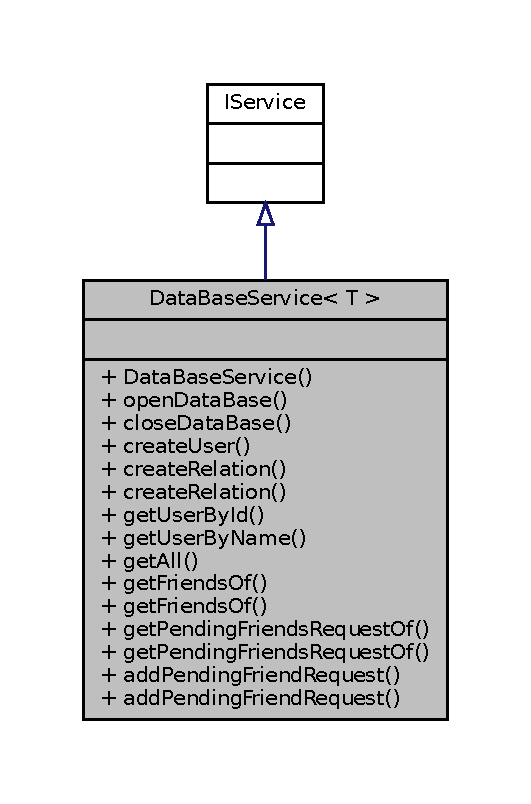
\includegraphics[width=255pt]{classDataBaseService__inherit__graph}
\end{center}
\end{figure}


Collaboration diagram for Data\+Base\+Service$<$ T $>$\+:
\nopagebreak
\begin{figure}[H]
\begin{center}
\leavevmode
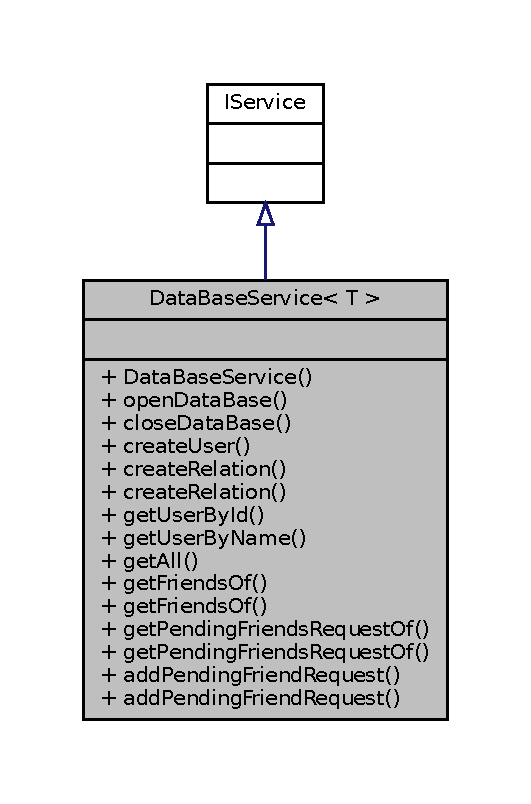
\includegraphics[width=255pt]{classDataBaseService__coll__graph}
\end{center}
\end{figure}
\subsection*{Public Member Functions}
\begin{DoxyCompactItemize}
\item 
\mbox{\hyperlink{classDataBaseService_ac5820e66451a0393723eb87db0c98c97}{Data\+Base\+Service}} ()
\item 
bool \mbox{\hyperlink{classDataBaseService_a0f1095843e3650701cdd23ae8dbc09d8}{open\+Data\+Base}} (const std\+::string \&name=\mbox{\hyperlink{DataBaseService_8hpp_aed391e0e48987704aefc7aa59b508aa7}{D\+A\+T\+A\+B\+A\+S\+E\+\_\+\+D\+E\+F\+A\+U\+L\+T\+\_\+\+N\+A\+ME}})
\item 
bool \mbox{\hyperlink{classDataBaseService_a1106f4f3393298f38e66b8a7b6bc5dc1}{close\+Data\+Base}} ()
\item 
bool \mbox{\hyperlink{classDataBaseService_af13f9198530eda7dae7d4308ea25258c}{create\+User}} (const std\+::string \&username, const std\+::string \&password)
\item 
bool \mbox{\hyperlink{classDataBaseService_a1c133b9b35bb83281c96a1ccbf08aa5f}{create\+Relation}} (int a, int b)
\item 
bool \mbox{\hyperlink{classDataBaseService_a72fd8d920d0483b01db15518fa578e15}{create\+Relation}} (const std\+::string \&username1, const std\+::string \&username2)
\item 
\mbox{\hyperlink{structUser}{User}} \mbox{\hyperlink{classDataBaseService_a04a13e93541e53fa750bf169ec0b5b85}{get\+User\+By\+Id}} (int id)
\item 
\mbox{\hyperlink{structUser}{User}} \mbox{\hyperlink{classDataBaseService_a1e0272ebe8dd31859b810e6f797cde5b}{get\+User\+By\+Name}} (const std\+::string \&username)
\item 
std\+::vector$<$ \mbox{\hyperlink{structUser}{User}} $>$ \mbox{\hyperlink{classDataBaseService_a1226c799e69e1417202366d4c2f7137d}{get\+All}} ()
\item 
std\+::vector$<$ \mbox{\hyperlink{structUser}{User}} $>$ \mbox{\hyperlink{classDataBaseService_ac82ba94d3e80ccc2f576b14bf71c8c2e}{get\+Friends\+Of}} (int id)
\item 
std\+::vector$<$ \mbox{\hyperlink{structUser}{User}} $>$ \mbox{\hyperlink{classDataBaseService_a11c94f12e798e1bf70afa4581fa7c8b0}{get\+Friends\+Of}} (const std\+::string \&username)
\item 
std\+::vector$<$ \mbox{\hyperlink{structPendingFriendRequest}{Pending\+Friend\+Request}} $>$ \mbox{\hyperlink{classDataBaseService_a14110b164fa5ae2af7edb53ba58f38df}{get\+Pending\+Friends\+Request\+Of}} (int id)
\item 
std\+::vector$<$ \mbox{\hyperlink{structPendingFriendRequest}{Pending\+Friend\+Request}} $>$ \mbox{\hyperlink{classDataBaseService_a96fb5a08a7337b7c2728317d445fc923}{get\+Pending\+Friends\+Request\+Of}} (const std\+::string \&username)
\item 
bool \mbox{\hyperlink{classDataBaseService_a1f31c3e831b50028eccfe4bbc6fce6cd}{add\+Pending\+Friend\+Request}} (int sender, int receiver)
\item 
bool \mbox{\hyperlink{classDataBaseService_a655fd576cba8952f982546adacaa6e57}{add\+Pending\+Friend\+Request}} (const std\+::string \&sender, const std\+::string \&receiver)
\end{DoxyCompactItemize}


\subsection{Constructor \& Destructor Documentation}
\mbox{\Hypertarget{classDataBaseService_ac5820e66451a0393723eb87db0c98c97}\label{classDataBaseService_ac5820e66451a0393723eb87db0c98c97}} 
\index{Data\+Base\+Service@{Data\+Base\+Service}!Data\+Base\+Service@{Data\+Base\+Service}}
\index{Data\+Base\+Service@{Data\+Base\+Service}!Data\+Base\+Service@{Data\+Base\+Service}}
\subsubsection{\texorpdfstring{Data\+Base\+Service()}{DataBaseService()}}
{\footnotesize\ttfamily template$<$class T $>$ \\
\mbox{\hyperlink{classDataBaseService}{Data\+Base\+Service}}$<$ T $>$\+::\mbox{\hyperlink{classDataBaseService}{Data\+Base\+Service}} (\begin{DoxyParamCaption}{ }\end{DoxyParamCaption})\hspace{0.3cm}{\ttfamily [inline]}, {\ttfamily [explicit]}}



\subsection{Member Function Documentation}
\mbox{\Hypertarget{classDataBaseService_a1f31c3e831b50028eccfe4bbc6fce6cd}\label{classDataBaseService_a1f31c3e831b50028eccfe4bbc6fce6cd}} 
\index{Data\+Base\+Service@{Data\+Base\+Service}!add\+Pending\+Friend\+Request@{add\+Pending\+Friend\+Request}}
\index{add\+Pending\+Friend\+Request@{add\+Pending\+Friend\+Request}!Data\+Base\+Service@{Data\+Base\+Service}}
\subsubsection{\texorpdfstring{add\+Pending\+Friend\+Request()}{addPendingFriendRequest()}\hspace{0.1cm}{\footnotesize\ttfamily [1/2]}}
{\footnotesize\ttfamily template$<$class T $>$ \\
bool \mbox{\hyperlink{classDataBaseService}{Data\+Base\+Service}}$<$ T $>$\+::add\+Pending\+Friend\+Request (\begin{DoxyParamCaption}\item[{int}]{sender,  }\item[{int}]{receiver }\end{DoxyParamCaption})\hspace{0.3cm}{\ttfamily [inline]}}

\mbox{\Hypertarget{classDataBaseService_a655fd576cba8952f982546adacaa6e57}\label{classDataBaseService_a655fd576cba8952f982546adacaa6e57}} 
\index{Data\+Base\+Service@{Data\+Base\+Service}!add\+Pending\+Friend\+Request@{add\+Pending\+Friend\+Request}}
\index{add\+Pending\+Friend\+Request@{add\+Pending\+Friend\+Request}!Data\+Base\+Service@{Data\+Base\+Service}}
\subsubsection{\texorpdfstring{add\+Pending\+Friend\+Request()}{addPendingFriendRequest()}\hspace{0.1cm}{\footnotesize\ttfamily [2/2]}}
{\footnotesize\ttfamily template$<$class T $>$ \\
bool \mbox{\hyperlink{classDataBaseService}{Data\+Base\+Service}}$<$ T $>$\+::add\+Pending\+Friend\+Request (\begin{DoxyParamCaption}\item[{const std\+::string \&}]{sender,  }\item[{const std\+::string \&}]{receiver }\end{DoxyParamCaption})\hspace{0.3cm}{\ttfamily [inline]}}

\mbox{\Hypertarget{classDataBaseService_a1106f4f3393298f38e66b8a7b6bc5dc1}\label{classDataBaseService_a1106f4f3393298f38e66b8a7b6bc5dc1}} 
\index{Data\+Base\+Service@{Data\+Base\+Service}!close\+Data\+Base@{close\+Data\+Base}}
\index{close\+Data\+Base@{close\+Data\+Base}!Data\+Base\+Service@{Data\+Base\+Service}}
\subsubsection{\texorpdfstring{close\+Data\+Base()}{closeDataBase()}}
{\footnotesize\ttfamily template$<$class T $>$ \\
bool \mbox{\hyperlink{classDataBaseService}{Data\+Base\+Service}}$<$ T $>$\+::close\+Data\+Base (\begin{DoxyParamCaption}{ }\end{DoxyParamCaption})\hspace{0.3cm}{\ttfamily [inline]}}

\mbox{\Hypertarget{classDataBaseService_a1c133b9b35bb83281c96a1ccbf08aa5f}\label{classDataBaseService_a1c133b9b35bb83281c96a1ccbf08aa5f}} 
\index{Data\+Base\+Service@{Data\+Base\+Service}!create\+Relation@{create\+Relation}}
\index{create\+Relation@{create\+Relation}!Data\+Base\+Service@{Data\+Base\+Service}}
\subsubsection{\texorpdfstring{create\+Relation()}{createRelation()}\hspace{0.1cm}{\footnotesize\ttfamily [1/2]}}
{\footnotesize\ttfamily template$<$class T $>$ \\
bool \mbox{\hyperlink{classDataBaseService}{Data\+Base\+Service}}$<$ T $>$\+::create\+Relation (\begin{DoxyParamCaption}\item[{int}]{a,  }\item[{int}]{b }\end{DoxyParamCaption})\hspace{0.3cm}{\ttfamily [inline]}}

\mbox{\Hypertarget{classDataBaseService_a72fd8d920d0483b01db15518fa578e15}\label{classDataBaseService_a72fd8d920d0483b01db15518fa578e15}} 
\index{Data\+Base\+Service@{Data\+Base\+Service}!create\+Relation@{create\+Relation}}
\index{create\+Relation@{create\+Relation}!Data\+Base\+Service@{Data\+Base\+Service}}
\subsubsection{\texorpdfstring{create\+Relation()}{createRelation()}\hspace{0.1cm}{\footnotesize\ttfamily [2/2]}}
{\footnotesize\ttfamily template$<$class T $>$ \\
bool \mbox{\hyperlink{classDataBaseService}{Data\+Base\+Service}}$<$ T $>$\+::create\+Relation (\begin{DoxyParamCaption}\item[{const std\+::string \&}]{username1,  }\item[{const std\+::string \&}]{username2 }\end{DoxyParamCaption})\hspace{0.3cm}{\ttfamily [inline]}}

\mbox{\Hypertarget{classDataBaseService_af13f9198530eda7dae7d4308ea25258c}\label{classDataBaseService_af13f9198530eda7dae7d4308ea25258c}} 
\index{Data\+Base\+Service@{Data\+Base\+Service}!create\+User@{create\+User}}
\index{create\+User@{create\+User}!Data\+Base\+Service@{Data\+Base\+Service}}
\subsubsection{\texorpdfstring{create\+User()}{createUser()}}
{\footnotesize\ttfamily template$<$class T $>$ \\
bool \mbox{\hyperlink{classDataBaseService}{Data\+Base\+Service}}$<$ T $>$\+::create\+User (\begin{DoxyParamCaption}\item[{const std\+::string \&}]{username,  }\item[{const std\+::string \&}]{password }\end{DoxyParamCaption})\hspace{0.3cm}{\ttfamily [inline]}}

\mbox{\Hypertarget{classDataBaseService_a1226c799e69e1417202366d4c2f7137d}\label{classDataBaseService_a1226c799e69e1417202366d4c2f7137d}} 
\index{Data\+Base\+Service@{Data\+Base\+Service}!get\+All@{get\+All}}
\index{get\+All@{get\+All}!Data\+Base\+Service@{Data\+Base\+Service}}
\subsubsection{\texorpdfstring{get\+All()}{getAll()}}
{\footnotesize\ttfamily template$<$class T $>$ \\
std\+::vector$<$\mbox{\hyperlink{structUser}{User}}$>$ \mbox{\hyperlink{classDataBaseService}{Data\+Base\+Service}}$<$ T $>$\+::get\+All (\begin{DoxyParamCaption}{ }\end{DoxyParamCaption})\hspace{0.3cm}{\ttfamily [inline]}}

\mbox{\Hypertarget{classDataBaseService_ac82ba94d3e80ccc2f576b14bf71c8c2e}\label{classDataBaseService_ac82ba94d3e80ccc2f576b14bf71c8c2e}} 
\index{Data\+Base\+Service@{Data\+Base\+Service}!get\+Friends\+Of@{get\+Friends\+Of}}
\index{get\+Friends\+Of@{get\+Friends\+Of}!Data\+Base\+Service@{Data\+Base\+Service}}
\subsubsection{\texorpdfstring{get\+Friends\+Of()}{getFriendsOf()}\hspace{0.1cm}{\footnotesize\ttfamily [1/2]}}
{\footnotesize\ttfamily template$<$class T $>$ \\
std\+::vector$<$\mbox{\hyperlink{structUser}{User}}$>$ \mbox{\hyperlink{classDataBaseService}{Data\+Base\+Service}}$<$ T $>$\+::get\+Friends\+Of (\begin{DoxyParamCaption}\item[{int}]{id }\end{DoxyParamCaption})\hspace{0.3cm}{\ttfamily [inline]}}

\mbox{\Hypertarget{classDataBaseService_a11c94f12e798e1bf70afa4581fa7c8b0}\label{classDataBaseService_a11c94f12e798e1bf70afa4581fa7c8b0}} 
\index{Data\+Base\+Service@{Data\+Base\+Service}!get\+Friends\+Of@{get\+Friends\+Of}}
\index{get\+Friends\+Of@{get\+Friends\+Of}!Data\+Base\+Service@{Data\+Base\+Service}}
\subsubsection{\texorpdfstring{get\+Friends\+Of()}{getFriendsOf()}\hspace{0.1cm}{\footnotesize\ttfamily [2/2]}}
{\footnotesize\ttfamily template$<$class T $>$ \\
std\+::vector$<$\mbox{\hyperlink{structUser}{User}}$>$ \mbox{\hyperlink{classDataBaseService}{Data\+Base\+Service}}$<$ T $>$\+::get\+Friends\+Of (\begin{DoxyParamCaption}\item[{const std\+::string \&}]{username }\end{DoxyParamCaption})\hspace{0.3cm}{\ttfamily [inline]}}

\mbox{\Hypertarget{classDataBaseService_a14110b164fa5ae2af7edb53ba58f38df}\label{classDataBaseService_a14110b164fa5ae2af7edb53ba58f38df}} 
\index{Data\+Base\+Service@{Data\+Base\+Service}!get\+Pending\+Friends\+Request\+Of@{get\+Pending\+Friends\+Request\+Of}}
\index{get\+Pending\+Friends\+Request\+Of@{get\+Pending\+Friends\+Request\+Of}!Data\+Base\+Service@{Data\+Base\+Service}}
\subsubsection{\texorpdfstring{get\+Pending\+Friends\+Request\+Of()}{getPendingFriendsRequestOf()}\hspace{0.1cm}{\footnotesize\ttfamily [1/2]}}
{\footnotesize\ttfamily template$<$class T $>$ \\
std\+::vector$<$\mbox{\hyperlink{structPendingFriendRequest}{Pending\+Friend\+Request}}$>$ \mbox{\hyperlink{classDataBaseService}{Data\+Base\+Service}}$<$ T $>$\+::get\+Pending\+Friends\+Request\+Of (\begin{DoxyParamCaption}\item[{int}]{id }\end{DoxyParamCaption})\hspace{0.3cm}{\ttfamily [inline]}}

\mbox{\Hypertarget{classDataBaseService_a96fb5a08a7337b7c2728317d445fc923}\label{classDataBaseService_a96fb5a08a7337b7c2728317d445fc923}} 
\index{Data\+Base\+Service@{Data\+Base\+Service}!get\+Pending\+Friends\+Request\+Of@{get\+Pending\+Friends\+Request\+Of}}
\index{get\+Pending\+Friends\+Request\+Of@{get\+Pending\+Friends\+Request\+Of}!Data\+Base\+Service@{Data\+Base\+Service}}
\subsubsection{\texorpdfstring{get\+Pending\+Friends\+Request\+Of()}{getPendingFriendsRequestOf()}\hspace{0.1cm}{\footnotesize\ttfamily [2/2]}}
{\footnotesize\ttfamily template$<$class T $>$ \\
std\+::vector$<$\mbox{\hyperlink{structPendingFriendRequest}{Pending\+Friend\+Request}}$>$ \mbox{\hyperlink{classDataBaseService}{Data\+Base\+Service}}$<$ T $>$\+::get\+Pending\+Friends\+Request\+Of (\begin{DoxyParamCaption}\item[{const std\+::string \&}]{username }\end{DoxyParamCaption})\hspace{0.3cm}{\ttfamily [inline]}}

\mbox{\Hypertarget{classDataBaseService_a04a13e93541e53fa750bf169ec0b5b85}\label{classDataBaseService_a04a13e93541e53fa750bf169ec0b5b85}} 
\index{Data\+Base\+Service@{Data\+Base\+Service}!get\+User\+By\+Id@{get\+User\+By\+Id}}
\index{get\+User\+By\+Id@{get\+User\+By\+Id}!Data\+Base\+Service@{Data\+Base\+Service}}
\subsubsection{\texorpdfstring{get\+User\+By\+Id()}{getUserById()}}
{\footnotesize\ttfamily template$<$class T $>$ \\
\mbox{\hyperlink{structUser}{User}} \mbox{\hyperlink{classDataBaseService}{Data\+Base\+Service}}$<$ T $>$\+::get\+User\+By\+Id (\begin{DoxyParamCaption}\item[{int}]{id }\end{DoxyParamCaption})\hspace{0.3cm}{\ttfamily [inline]}}

\mbox{\Hypertarget{classDataBaseService_a1e0272ebe8dd31859b810e6f797cde5b}\label{classDataBaseService_a1e0272ebe8dd31859b810e6f797cde5b}} 
\index{Data\+Base\+Service@{Data\+Base\+Service}!get\+User\+By\+Name@{get\+User\+By\+Name}}
\index{get\+User\+By\+Name@{get\+User\+By\+Name}!Data\+Base\+Service@{Data\+Base\+Service}}
\subsubsection{\texorpdfstring{get\+User\+By\+Name()}{getUserByName()}}
{\footnotesize\ttfamily template$<$class T $>$ \\
\mbox{\hyperlink{structUser}{User}} \mbox{\hyperlink{classDataBaseService}{Data\+Base\+Service}}$<$ T $>$\+::get\+User\+By\+Name (\begin{DoxyParamCaption}\item[{const std\+::string \&}]{username }\end{DoxyParamCaption})\hspace{0.3cm}{\ttfamily [inline]}}

\mbox{\Hypertarget{classDataBaseService_a0f1095843e3650701cdd23ae8dbc09d8}\label{classDataBaseService_a0f1095843e3650701cdd23ae8dbc09d8}} 
\index{Data\+Base\+Service@{Data\+Base\+Service}!open\+Data\+Base@{open\+Data\+Base}}
\index{open\+Data\+Base@{open\+Data\+Base}!Data\+Base\+Service@{Data\+Base\+Service}}
\subsubsection{\texorpdfstring{open\+Data\+Base()}{openDataBase()}}
{\footnotesize\ttfamily template$<$class T $>$ \\
bool \mbox{\hyperlink{classDataBaseService}{Data\+Base\+Service}}$<$ T $>$\+::open\+Data\+Base (\begin{DoxyParamCaption}\item[{const std\+::string \&}]{name = {\ttfamily \mbox{\hyperlink{DataBaseService_8hpp_aed391e0e48987704aefc7aa59b508aa7}{D\+A\+T\+A\+B\+A\+S\+E\+\_\+\+D\+E\+F\+A\+U\+L\+T\+\_\+\+N\+A\+ME}}} }\end{DoxyParamCaption})\hspace{0.3cm}{\ttfamily [inline]}}



The documentation for this class was generated from the following file\+:\begin{DoxyCompactItemize}
\item 
services/\mbox{\hyperlink{DataBaseService_8hpp}{Data\+Base\+Service.\+hpp}}\end{DoxyCompactItemize}

\hypertarget{structDispatchData}{}\section{Dispatch\+Data Struct Reference}
\label{structDispatchData}\index{Dispatch\+Data@{Dispatch\+Data}}


{\ttfamily \#include $<$Dispatch\+Service.\+hpp$>$}



Collaboration diagram for Dispatch\+Data\+:
\nopagebreak
\begin{figure}[H]
\begin{center}
\leavevmode
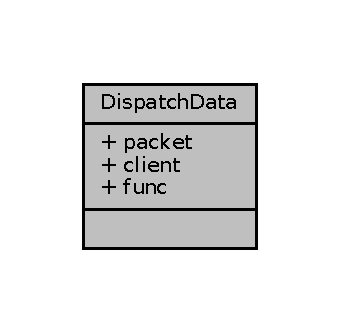
\includegraphics[width=163pt]{structDispatchData__coll__graph}
\end{center}
\end{figure}
\subsection*{Public Attributes}
\begin{DoxyCompactItemize}
\item 
std\+::unique\+\_\+ptr$<$ I\+Packet $>$ \mbox{\hyperlink{structDispatchData_a73c4113d390c2df0b035e7e89ea829b4}{packet}}
\item 
boost\+::shared\+\_\+ptr$<$ \mbox{\hyperlink{classClient}{Client}} $>$ \mbox{\hyperlink{structDispatchData_a05f2c90200f8ef88bd63f3a7f63aa630}{client}}
\item 
std\+::function$<$ void(boost\+::shared\+\_\+ptr$<$ \mbox{\hyperlink{classClient}{Client}} $>$, std\+::unique\+\_\+ptr$<$ I\+Packet $>$ \&)$>$ \mbox{\hyperlink{structDispatchData_a6672e8f2dfa81cd5b386c1cc96a1c2f6}{func}}
\end{DoxyCompactItemize}


\subsection{Member Data Documentation}
\mbox{\Hypertarget{structDispatchData_a05f2c90200f8ef88bd63f3a7f63aa630}\label{structDispatchData_a05f2c90200f8ef88bd63f3a7f63aa630}} 
\index{Dispatch\+Data@{Dispatch\+Data}!client@{client}}
\index{client@{client}!Dispatch\+Data@{Dispatch\+Data}}
\subsubsection{\texorpdfstring{client}{client}}
{\footnotesize\ttfamily boost\+::shared\+\_\+ptr$<$\mbox{\hyperlink{classClient}{Client}}$>$ Dispatch\+Data\+::client}

\mbox{\Hypertarget{structDispatchData_a6672e8f2dfa81cd5b386c1cc96a1c2f6}\label{structDispatchData_a6672e8f2dfa81cd5b386c1cc96a1c2f6}} 
\index{Dispatch\+Data@{Dispatch\+Data}!func@{func}}
\index{func@{func}!Dispatch\+Data@{Dispatch\+Data}}
\subsubsection{\texorpdfstring{func}{func}}
{\footnotesize\ttfamily std\+::function$<$void(boost\+::shared\+\_\+ptr$<$\mbox{\hyperlink{classClient}{Client}}$>$, std\+::unique\+\_\+ptr$<$I\+Packet$>$ \&)$>$ Dispatch\+Data\+::func}

\mbox{\Hypertarget{structDispatchData_a73c4113d390c2df0b035e7e89ea829b4}\label{structDispatchData_a73c4113d390c2df0b035e7e89ea829b4}} 
\index{Dispatch\+Data@{Dispatch\+Data}!packet@{packet}}
\index{packet@{packet}!Dispatch\+Data@{Dispatch\+Data}}
\subsubsection{\texorpdfstring{packet}{packet}}
{\footnotesize\ttfamily std\+::unique\+\_\+ptr$<$I\+Packet$>$ Dispatch\+Data\+::packet}



The documentation for this struct was generated from the following file\+:\begin{DoxyCompactItemize}
\item 
services/\mbox{\hyperlink{DispatchService_8hpp}{Dispatch\+Service.\+hpp}}\end{DoxyCompactItemize}

\hypertarget{classDispatchService}{}\section{Dispatch\+Service Class Reference}
\label{classDispatchService}\index{Dispatch\+Service@{Dispatch\+Service}}


{\ttfamily \#include $<$Dispatch\+Service.\+hpp$>$}



Inheritance diagram for Dispatch\+Service\+:
\nopagebreak
\begin{figure}[H]
\begin{center}
\leavevmode
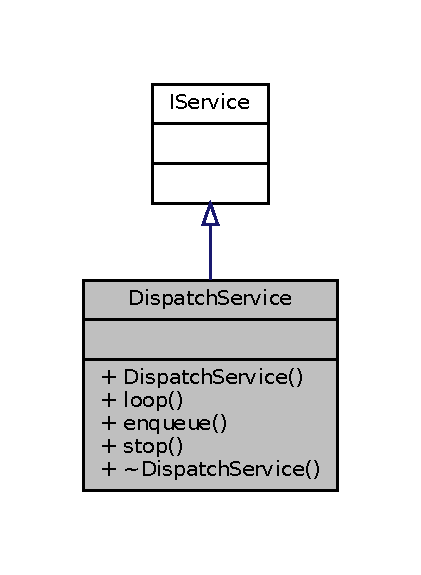
\includegraphics[width=202pt]{classDispatchService__inherit__graph}
\end{center}
\end{figure}


Collaboration diagram for Dispatch\+Service\+:
\nopagebreak
\begin{figure}[H]
\begin{center}
\leavevmode
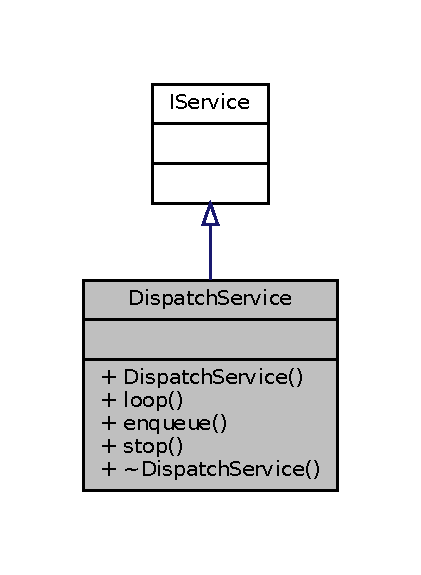
\includegraphics[width=202pt]{classDispatchService__coll__graph}
\end{center}
\end{figure}
\subsection*{Public Member Functions}
\begin{DoxyCompactItemize}
\item 
\mbox{\hyperlink{classDispatchService_a71022bcc29c8a76ac2af156c369ef116}{Dispatch\+Service}} ()
\item 
void \mbox{\hyperlink{classDispatchService_aa7b4c44dbb842aa208e4109da6c68465}{loop}} ()
\item 
void \mbox{\hyperlink{classDispatchService_a0180e712e67d8062499f25a49747c1f8}{enqueue}} (\mbox{\hyperlink{structDispatchData}{Dispatch\+Data}} \&data)
\item 
void \mbox{\hyperlink{classDispatchService_ab0fac2c10f5d1dd90847736cab05fb10}{stop}} ()
\item 
\mbox{\hyperlink{classDispatchService_a7a4866bbec833ad0e8074ef8170de286}{$\sim$\+Dispatch\+Service}} ()
\end{DoxyCompactItemize}


\subsection{Constructor \& Destructor Documentation}
\mbox{\Hypertarget{classDispatchService_a71022bcc29c8a76ac2af156c369ef116}\label{classDispatchService_a71022bcc29c8a76ac2af156c369ef116}} 
\index{Dispatch\+Service@{Dispatch\+Service}!Dispatch\+Service@{Dispatch\+Service}}
\index{Dispatch\+Service@{Dispatch\+Service}!Dispatch\+Service@{Dispatch\+Service}}
\subsubsection{\texorpdfstring{Dispatch\+Service()}{DispatchService()}}
{\footnotesize\ttfamily Dispatch\+Service\+::\+Dispatch\+Service (\begin{DoxyParamCaption}{ }\end{DoxyParamCaption})\hspace{0.3cm}{\ttfamily [inline]}}

Here is the call graph for this function\+:
\nopagebreak
\begin{figure}[H]
\begin{center}
\leavevmode
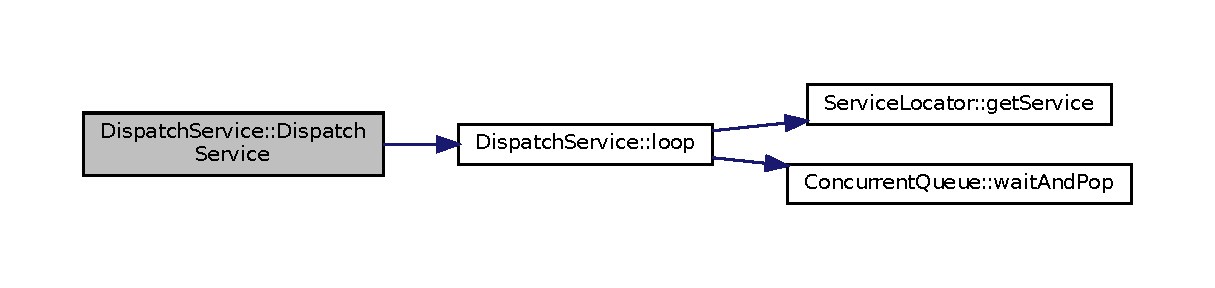
\includegraphics[width=350pt]{classDispatchService_a71022bcc29c8a76ac2af156c369ef116_cgraph}
\end{center}
\end{figure}
\mbox{\Hypertarget{classDispatchService_a7a4866bbec833ad0e8074ef8170de286}\label{classDispatchService_a7a4866bbec833ad0e8074ef8170de286}} 
\index{Dispatch\+Service@{Dispatch\+Service}!````~Dispatch\+Service@{$\sim$\+Dispatch\+Service}}
\index{````~Dispatch\+Service@{$\sim$\+Dispatch\+Service}!Dispatch\+Service@{Dispatch\+Service}}
\subsubsection{\texorpdfstring{$\sim$\+Dispatch\+Service()}{~DispatchService()}}
{\footnotesize\ttfamily Dispatch\+Service\+::$\sim$\+Dispatch\+Service (\begin{DoxyParamCaption}{ }\end{DoxyParamCaption})\hspace{0.3cm}{\ttfamily [inline]}}



\subsection{Member Function Documentation}
\mbox{\Hypertarget{classDispatchService_a0180e712e67d8062499f25a49747c1f8}\label{classDispatchService_a0180e712e67d8062499f25a49747c1f8}} 
\index{Dispatch\+Service@{Dispatch\+Service}!enqueue@{enqueue}}
\index{enqueue@{enqueue}!Dispatch\+Service@{Dispatch\+Service}}
\subsubsection{\texorpdfstring{enqueue()}{enqueue()}}
{\footnotesize\ttfamily void Dispatch\+Service\+::enqueue (\begin{DoxyParamCaption}\item[{\mbox{\hyperlink{structDispatchData}{Dispatch\+Data}} \&}]{data }\end{DoxyParamCaption})\hspace{0.3cm}{\ttfamily [inline]}}

Here is the call graph for this function\+:
\nopagebreak
\begin{figure}[H]
\begin{center}
\leavevmode
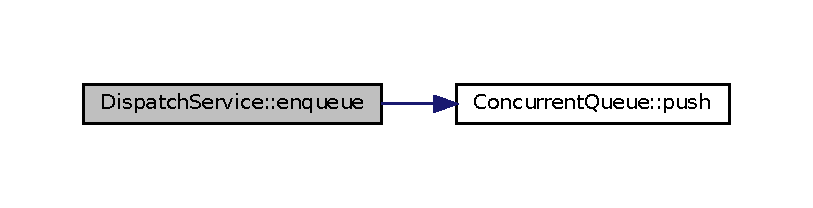
\includegraphics[width=350pt]{classDispatchService_a0180e712e67d8062499f25a49747c1f8_cgraph}
\end{center}
\end{figure}
\mbox{\Hypertarget{classDispatchService_aa7b4c44dbb842aa208e4109da6c68465}\label{classDispatchService_aa7b4c44dbb842aa208e4109da6c68465}} 
\index{Dispatch\+Service@{Dispatch\+Service}!loop@{loop}}
\index{loop@{loop}!Dispatch\+Service@{Dispatch\+Service}}
\subsubsection{\texorpdfstring{loop()}{loop()}}
{\footnotesize\ttfamily void Dispatch\+Service\+::loop (\begin{DoxyParamCaption}{ }\end{DoxyParamCaption})\hspace{0.3cm}{\ttfamily [inline]}}

Here is the call graph for this function\+:
\nopagebreak
\begin{figure}[H]
\begin{center}
\leavevmode
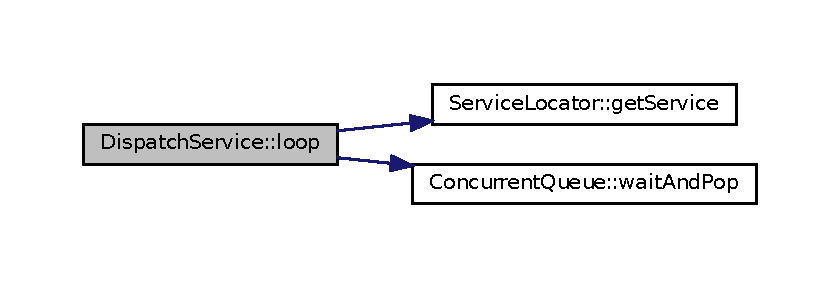
\includegraphics[width=350pt]{classDispatchService_aa7b4c44dbb842aa208e4109da6c68465_cgraph}
\end{center}
\end{figure}
\mbox{\Hypertarget{classDispatchService_ab0fac2c10f5d1dd90847736cab05fb10}\label{classDispatchService_ab0fac2c10f5d1dd90847736cab05fb10}} 
\index{Dispatch\+Service@{Dispatch\+Service}!stop@{stop}}
\index{stop@{stop}!Dispatch\+Service@{Dispatch\+Service}}
\subsubsection{\texorpdfstring{stop()}{stop()}}
{\footnotesize\ttfamily void Dispatch\+Service\+::stop (\begin{DoxyParamCaption}{ }\end{DoxyParamCaption})\hspace{0.3cm}{\ttfamily [inline]}}



The documentation for this class was generated from the following file\+:\begin{DoxyCompactItemize}
\item 
services/\mbox{\hyperlink{DispatchService_8hpp}{Dispatch\+Service.\+hpp}}\end{DoxyCompactItemize}

\hypertarget{structFriendship}{}\section{Friendship Struct Reference}
\label{structFriendship}\index{Friendship@{Friendship}}


{\ttfamily \#include $<$Sqlite\+Provider.\+hpp$>$}



Collaboration diagram for Friendship\+:
\nopagebreak
\begin{figure}[H]
\begin{center}
\leavevmode
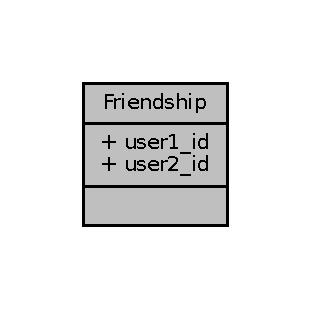
\includegraphics[width=149pt]{structFriendship__coll__graph}
\end{center}
\end{figure}
\subsection*{Public Attributes}
\begin{DoxyCompactItemize}
\item 
int \mbox{\hyperlink{structFriendship_a1b9f466250defc4657029df09bb2ca62}{user1\+\_\+id}}
\item 
int \mbox{\hyperlink{structFriendship_a673079868906404d4c283b682934e501}{user2\+\_\+id}}
\end{DoxyCompactItemize}


\subsection{Member Data Documentation}
\mbox{\Hypertarget{structFriendship_a1b9f466250defc4657029df09bb2ca62}\label{structFriendship_a1b9f466250defc4657029df09bb2ca62}} 
\index{Friendship@{Friendship}!user1\+\_\+id@{user1\+\_\+id}}
\index{user1\+\_\+id@{user1\+\_\+id}!Friendship@{Friendship}}
\subsubsection{\texorpdfstring{user1\+\_\+id}{user1\_id}}
{\footnotesize\ttfamily int Friendship\+::user1\+\_\+id}

\mbox{\Hypertarget{structFriendship_a673079868906404d4c283b682934e501}\label{structFriendship_a673079868906404d4c283b682934e501}} 
\index{Friendship@{Friendship}!user2\+\_\+id@{user2\+\_\+id}}
\index{user2\+\_\+id@{user2\+\_\+id}!Friendship@{Friendship}}
\subsubsection{\texorpdfstring{user2\+\_\+id}{user2\_id}}
{\footnotesize\ttfamily int Friendship\+::user2\+\_\+id}



The documentation for this struct was generated from the following file\+:\begin{DoxyCompactItemize}
\item 
database/\mbox{\hyperlink{SqliteProvider_8hpp}{Sqlite\+Provider.\+hpp}}\end{DoxyCompactItemize}

\hypertarget{classHandlerService}{}\section{Handler\+Service Class Reference}
\label{classHandlerService}\index{Handler\+Service@{Handler\+Service}}


{\ttfamily \#include $<$Handler\+Service.\+hpp$>$}



Inheritance diagram for Handler\+Service\+:
\nopagebreak
\begin{figure}[H]
\begin{center}
\leavevmode
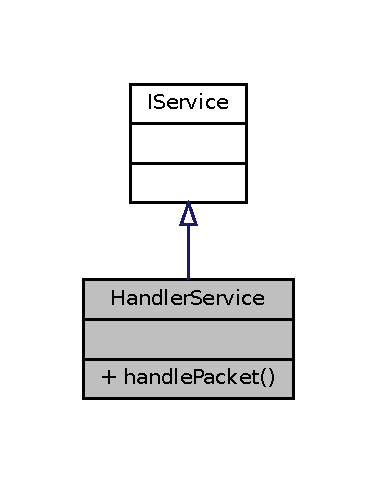
\includegraphics[width=181pt]{classHandlerService__inherit__graph}
\end{center}
\end{figure}


Collaboration diagram for Handler\+Service\+:
\nopagebreak
\begin{figure}[H]
\begin{center}
\leavevmode
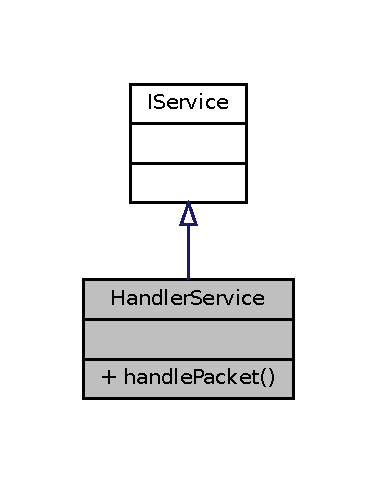
\includegraphics[width=181pt]{classHandlerService__coll__graph}
\end{center}
\end{figure}
\subsection*{Public Member Functions}
\begin{DoxyCompactItemize}
\item 
void \mbox{\hyperlink{classHandlerService_a4d688250d26b4300f3de63412308440e}{handle\+Packet}} (boost\+::shared\+\_\+ptr$<$ \mbox{\hyperlink{classIConnection}{I\+Connection}} $>$ \&connection, void $\ast$data, size\+\_\+t len)
\end{DoxyCompactItemize}


\subsection{Member Function Documentation}
\mbox{\Hypertarget{classHandlerService_a4d688250d26b4300f3de63412308440e}\label{classHandlerService_a4d688250d26b4300f3de63412308440e}} 
\index{Handler\+Service@{Handler\+Service}!handle\+Packet@{handle\+Packet}}
\index{handle\+Packet@{handle\+Packet}!Handler\+Service@{Handler\+Service}}
\subsubsection{\texorpdfstring{handle\+Packet()}{handlePacket()}}
{\footnotesize\ttfamily void Handler\+Service\+::handle\+Packet (\begin{DoxyParamCaption}\item[{boost\+::shared\+\_\+ptr$<$ \mbox{\hyperlink{classIConnection}{I\+Connection}} $>$ \&}]{connection,  }\item[{void $\ast$}]{data,  }\item[{size\+\_\+t}]{len }\end{DoxyParamCaption})\hspace{0.3cm}{\ttfamily [inline]}}

Here is the call graph for this function\+:
\nopagebreak
\begin{figure}[H]
\begin{center}
\leavevmode
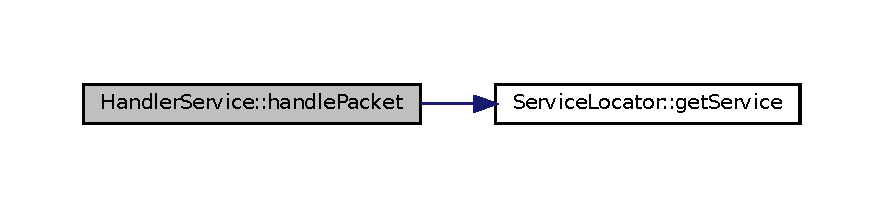
\includegraphics[width=350pt]{classHandlerService_a4d688250d26b4300f3de63412308440e_cgraph}
\end{center}
\end{figure}


The documentation for this class was generated from the following files\+:\begin{DoxyCompactItemize}
\item 
services/\mbox{\hyperlink{HandlerService_8hpp}{Handler\+Service.\+hpp}}\item 
services/\mbox{\hyperlink{HandlerService_8cpp}{Handler\+Service.\+cpp}}\end{DoxyCompactItemize}

\hypertarget{classHandshakeHandler}{}\section{Handshake\+Handler Class Reference}
\label{classHandshakeHandler}\index{Handshake\+Handler@{Handshake\+Handler}}


{\ttfamily \#include $<$Handshake\+Handler.\+hpp$>$}



Collaboration diagram for Handshake\+Handler\+:
\nopagebreak
\begin{figure}[H]
\begin{center}
\leavevmode
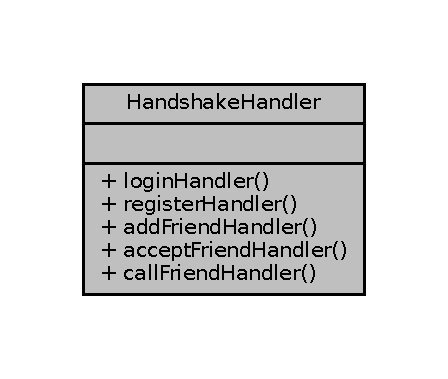
\includegraphics[width=215pt]{classHandshakeHandler__coll__graph}
\end{center}
\end{figure}
\subsection*{Static Public Member Functions}
\begin{DoxyCompactItemize}
\item 
static void \mbox{\hyperlink{classHandshakeHandler_aef80330a36ad493211e1a4b2e321f3f1}{login\+Handler}} (boost\+::shared\+\_\+ptr$<$ \mbox{\hyperlink{classClient}{Client}} $>$, std\+::unique\+\_\+ptr$<$ I\+Packet $>$ \&packet)
\item 
static void \mbox{\hyperlink{classHandshakeHandler_a1a93aa1ce4f7ca634f89dce9f30d29d8}{register\+Handler}} (boost\+::shared\+\_\+ptr$<$ \mbox{\hyperlink{classClient}{Client}} $>$, std\+::unique\+\_\+ptr$<$ I\+Packet $>$ \&packet)
\item 
static void \mbox{\hyperlink{classHandshakeHandler_aa0ebcde41ffa598adaa99c6e55389344}{add\+Friend\+Handler}} (boost\+::shared\+\_\+ptr$<$ \mbox{\hyperlink{classClient}{Client}} $>$, std\+::unique\+\_\+ptr$<$ I\+Packet $>$ \&packet)
\item 
static void \mbox{\hyperlink{classHandshakeHandler_a943b521a7ffadc5e339b9c32ced09c67}{accept\+Friend\+Handler}} (boost\+::shared\+\_\+ptr$<$ \mbox{\hyperlink{classClient}{Client}} $>$, std\+::unique\+\_\+ptr$<$ I\+Packet $>$ \&packet)
\item 
static void \mbox{\hyperlink{classHandshakeHandler_adeaf54ffd2fa8a3b6b9eb60a458b56e0}{call\+Friend\+Handler}} (boost\+::shared\+\_\+ptr$<$ \mbox{\hyperlink{classClient}{Client}} $>$, std\+::unique\+\_\+ptr$<$ I\+Packet $>$ \&packet)
\end{DoxyCompactItemize}


\subsection{Member Function Documentation}
\mbox{\Hypertarget{classHandshakeHandler_a943b521a7ffadc5e339b9c32ced09c67}\label{classHandshakeHandler_a943b521a7ffadc5e339b9c32ced09c67}} 
\index{Handshake\+Handler@{Handshake\+Handler}!accept\+Friend\+Handler@{accept\+Friend\+Handler}}
\index{accept\+Friend\+Handler@{accept\+Friend\+Handler}!Handshake\+Handler@{Handshake\+Handler}}
\subsubsection{\texorpdfstring{accept\+Friend\+Handler()}{acceptFriendHandler()}}
{\footnotesize\ttfamily void Handshake\+Handler\+::accept\+Friend\+Handler (\begin{DoxyParamCaption}\item[{boost\+::shared\+\_\+ptr$<$ \mbox{\hyperlink{classClient}{Client}} $>$}]{client,  }\item[{std\+::unique\+\_\+ptr$<$ I\+Packet $>$ \&}]{packet }\end{DoxyParamCaption})\hspace{0.3cm}{\ttfamily [static]}}

Here is the call graph for this function\+:
\nopagebreak
\begin{figure}[H]
\begin{center}
\leavevmode
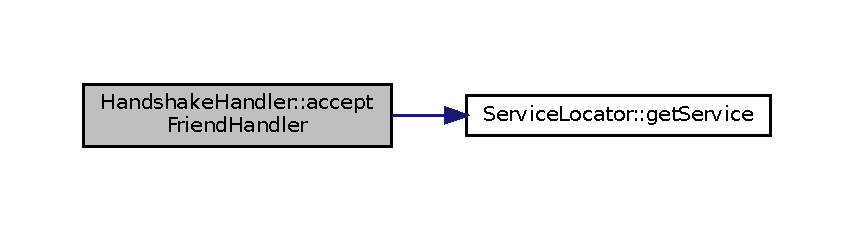
\includegraphics[width=350pt]{classHandshakeHandler_a943b521a7ffadc5e339b9c32ced09c67_cgraph}
\end{center}
\end{figure}
\mbox{\Hypertarget{classHandshakeHandler_aa0ebcde41ffa598adaa99c6e55389344}\label{classHandshakeHandler_aa0ebcde41ffa598adaa99c6e55389344}} 
\index{Handshake\+Handler@{Handshake\+Handler}!add\+Friend\+Handler@{add\+Friend\+Handler}}
\index{add\+Friend\+Handler@{add\+Friend\+Handler}!Handshake\+Handler@{Handshake\+Handler}}
\subsubsection{\texorpdfstring{add\+Friend\+Handler()}{addFriendHandler()}}
{\footnotesize\ttfamily void Handshake\+Handler\+::add\+Friend\+Handler (\begin{DoxyParamCaption}\item[{boost\+::shared\+\_\+ptr$<$ \mbox{\hyperlink{classClient}{Client}} $>$}]{client,  }\item[{std\+::unique\+\_\+ptr$<$ I\+Packet $>$ \&}]{packet }\end{DoxyParamCaption})\hspace{0.3cm}{\ttfamily [static]}}

Here is the call graph for this function\+:
\nopagebreak
\begin{figure}[H]
\begin{center}
\leavevmode
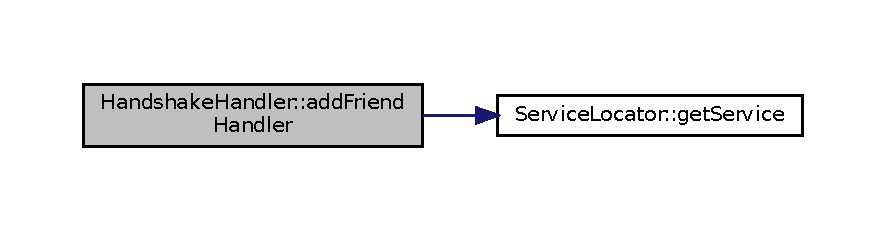
\includegraphics[width=350pt]{classHandshakeHandler_aa0ebcde41ffa598adaa99c6e55389344_cgraph}
\end{center}
\end{figure}
\mbox{\Hypertarget{classHandshakeHandler_adeaf54ffd2fa8a3b6b9eb60a458b56e0}\label{classHandshakeHandler_adeaf54ffd2fa8a3b6b9eb60a458b56e0}} 
\index{Handshake\+Handler@{Handshake\+Handler}!call\+Friend\+Handler@{call\+Friend\+Handler}}
\index{call\+Friend\+Handler@{call\+Friend\+Handler}!Handshake\+Handler@{Handshake\+Handler}}
\subsubsection{\texorpdfstring{call\+Friend\+Handler()}{callFriendHandler()}}
{\footnotesize\ttfamily void Handshake\+Handler\+::call\+Friend\+Handler (\begin{DoxyParamCaption}\item[{boost\+::shared\+\_\+ptr$<$ \mbox{\hyperlink{classClient}{Client}} $>$}]{client,  }\item[{std\+::unique\+\_\+ptr$<$ I\+Packet $>$ \&}]{packet }\end{DoxyParamCaption})\hspace{0.3cm}{\ttfamily [static]}}

Pour l\textquotesingle{}instant t\textquotesingle{}as pas le choix, si on t\textquotesingle{}appelle bah on t\textquotesingle{}appelle Here is the call graph for this function\+:
\nopagebreak
\begin{figure}[H]
\begin{center}
\leavevmode
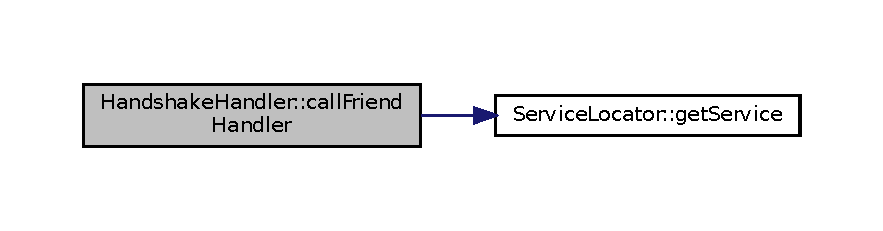
\includegraphics[width=350pt]{classHandshakeHandler_adeaf54ffd2fa8a3b6b9eb60a458b56e0_cgraph}
\end{center}
\end{figure}
\mbox{\Hypertarget{classHandshakeHandler_aef80330a36ad493211e1a4b2e321f3f1}\label{classHandshakeHandler_aef80330a36ad493211e1a4b2e321f3f1}} 
\index{Handshake\+Handler@{Handshake\+Handler}!login\+Handler@{login\+Handler}}
\index{login\+Handler@{login\+Handler}!Handshake\+Handler@{Handshake\+Handler}}
\subsubsection{\texorpdfstring{login\+Handler()}{loginHandler()}}
{\footnotesize\ttfamily void Handshake\+Handler\+::login\+Handler (\begin{DoxyParamCaption}\item[{boost\+::shared\+\_\+ptr$<$ \mbox{\hyperlink{classClient}{Client}} $>$}]{client,  }\item[{std\+::unique\+\_\+ptr$<$ I\+Packet $>$ \&}]{packet }\end{DoxyParamCaption})\hspace{0.3cm}{\ttfamily [static]}}

Here is the call graph for this function\+:
\nopagebreak
\begin{figure}[H]
\begin{center}
\leavevmode
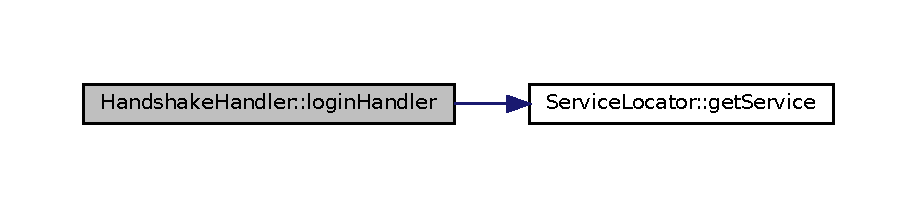
\includegraphics[width=350pt]{classHandshakeHandler_aef80330a36ad493211e1a4b2e321f3f1_cgraph}
\end{center}
\end{figure}
\mbox{\Hypertarget{classHandshakeHandler_a1a93aa1ce4f7ca634f89dce9f30d29d8}\label{classHandshakeHandler_a1a93aa1ce4f7ca634f89dce9f30d29d8}} 
\index{Handshake\+Handler@{Handshake\+Handler}!register\+Handler@{register\+Handler}}
\index{register\+Handler@{register\+Handler}!Handshake\+Handler@{Handshake\+Handler}}
\subsubsection{\texorpdfstring{register\+Handler()}{registerHandler()}}
{\footnotesize\ttfamily void Handshake\+Handler\+::register\+Handler (\begin{DoxyParamCaption}\item[{boost\+::shared\+\_\+ptr$<$ \mbox{\hyperlink{classClient}{Client}} $>$}]{client,  }\item[{std\+::unique\+\_\+ptr$<$ I\+Packet $>$ \&}]{packet }\end{DoxyParamCaption})\hspace{0.3cm}{\ttfamily [static]}}



The documentation for this class was generated from the following files\+:\begin{DoxyCompactItemize}
\item 
logic/handshake/\mbox{\hyperlink{HandshakeHandler_8hpp}{Handshake\+Handler.\+hpp}}\item 
logic/handshake/\mbox{\hyperlink{HandshakeHandler_8cpp}{Handshake\+Handler.\+cpp}}\end{DoxyCompactItemize}

\hypertarget{classIConnection}{}\section{I\+Connection Class Reference}
\label{classIConnection}\index{I\+Connection@{I\+Connection}}


{\ttfamily \#include $<$I\+Connection.\+hpp$>$}



Inheritance diagram for I\+Connection\+:
\nopagebreak
\begin{figure}[H]
\begin{center}
\leavevmode
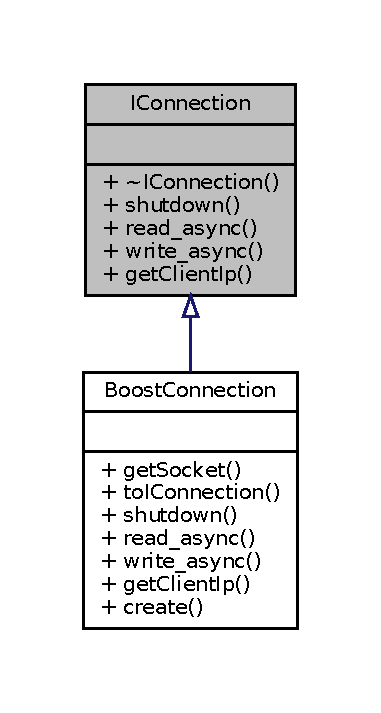
\includegraphics[width=183pt]{classIConnection__inherit__graph}
\end{center}
\end{figure}


Collaboration diagram for I\+Connection\+:
\nopagebreak
\begin{figure}[H]
\begin{center}
\leavevmode
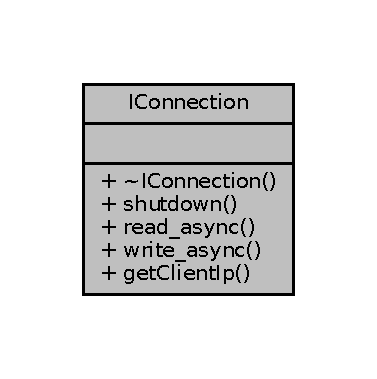
\includegraphics[width=181pt]{classIConnection__coll__graph}
\end{center}
\end{figure}
\subsection*{Public Member Functions}
\begin{DoxyCompactItemize}
\item 
virtual \mbox{\hyperlink{classIConnection_ad1c78f7f02b93d498d352ed5a2a5cd31}{$\sim$\+I\+Connection}} ()=default
\item 
virtual void \mbox{\hyperlink{classIConnection_ae15b6922f3a31a7f316a6390eb2469b2}{shutdown}} ()=0
\item 
virtual void \mbox{\hyperlink{classIConnection_a1c9d492241a79546f243088285279144}{read\+\_\+async}} ()=0
\item 
virtual void \mbox{\hyperlink{classIConnection_a7210f770ebae6277e98142a8b5a6226f}{write\+\_\+async}} (const std\+::string \&message)=0
\item 
virtual std\+::string \mbox{\hyperlink{classIConnection_a7064757e5c427496f482239dde7e0540}{get\+Client\+Ip}} () const =0
\end{DoxyCompactItemize}


\subsection{Constructor \& Destructor Documentation}
\mbox{\Hypertarget{classIConnection_ad1c78f7f02b93d498d352ed5a2a5cd31}\label{classIConnection_ad1c78f7f02b93d498d352ed5a2a5cd31}} 
\index{I\+Connection@{I\+Connection}!````~I\+Connection@{$\sim$\+I\+Connection}}
\index{````~I\+Connection@{$\sim$\+I\+Connection}!I\+Connection@{I\+Connection}}
\subsubsection{\texorpdfstring{$\sim$\+I\+Connection()}{~IConnection()}}
{\footnotesize\ttfamily virtual I\+Connection\+::$\sim$\+I\+Connection (\begin{DoxyParamCaption}{ }\end{DoxyParamCaption})\hspace{0.3cm}{\ttfamily [virtual]}, {\ttfamily [default]}}



\subsection{Member Function Documentation}
\mbox{\Hypertarget{classIConnection_a7064757e5c427496f482239dde7e0540}\label{classIConnection_a7064757e5c427496f482239dde7e0540}} 
\index{I\+Connection@{I\+Connection}!get\+Client\+Ip@{get\+Client\+Ip}}
\index{get\+Client\+Ip@{get\+Client\+Ip}!I\+Connection@{I\+Connection}}
\subsubsection{\texorpdfstring{get\+Client\+Ip()}{getClientIp()}}
{\footnotesize\ttfamily virtual std\+::string I\+Connection\+::get\+Client\+Ip (\begin{DoxyParamCaption}{ }\end{DoxyParamCaption}) const\hspace{0.3cm}{\ttfamily [pure virtual]}}



Implemented in \mbox{\hyperlink{classBoostConnection_a648ba5a8674fc95b4cab8c94225a19e9}{Boost\+Connection}}.

\mbox{\Hypertarget{classIConnection_a1c9d492241a79546f243088285279144}\label{classIConnection_a1c9d492241a79546f243088285279144}} 
\index{I\+Connection@{I\+Connection}!read\+\_\+async@{read\+\_\+async}}
\index{read\+\_\+async@{read\+\_\+async}!I\+Connection@{I\+Connection}}
\subsubsection{\texorpdfstring{read\+\_\+async()}{read\_async()}}
{\footnotesize\ttfamily virtual void I\+Connection\+::read\+\_\+async (\begin{DoxyParamCaption}{ }\end{DoxyParamCaption})\hspace{0.3cm}{\ttfamily [pure virtual]}}



Implemented in \mbox{\hyperlink{classBoostConnection_a8b117337238e2652adecde8971c1ab93}{Boost\+Connection}}.

\mbox{\Hypertarget{classIConnection_ae15b6922f3a31a7f316a6390eb2469b2}\label{classIConnection_ae15b6922f3a31a7f316a6390eb2469b2}} 
\index{I\+Connection@{I\+Connection}!shutdown@{shutdown}}
\index{shutdown@{shutdown}!I\+Connection@{I\+Connection}}
\subsubsection{\texorpdfstring{shutdown()}{shutdown()}}
{\footnotesize\ttfamily virtual void I\+Connection\+::shutdown (\begin{DoxyParamCaption}{ }\end{DoxyParamCaption})\hspace{0.3cm}{\ttfamily [pure virtual]}}



Implemented in \mbox{\hyperlink{classBoostConnection_a576ca28ef2f8f335ee1a0ccab64cc55b}{Boost\+Connection}}.

\mbox{\Hypertarget{classIConnection_a7210f770ebae6277e98142a8b5a6226f}\label{classIConnection_a7210f770ebae6277e98142a8b5a6226f}} 
\index{I\+Connection@{I\+Connection}!write\+\_\+async@{write\+\_\+async}}
\index{write\+\_\+async@{write\+\_\+async}!I\+Connection@{I\+Connection}}
\subsubsection{\texorpdfstring{write\+\_\+async()}{write\_async()}}
{\footnotesize\ttfamily virtual void I\+Connection\+::write\+\_\+async (\begin{DoxyParamCaption}\item[{const std\+::string \&}]{message }\end{DoxyParamCaption})\hspace{0.3cm}{\ttfamily [pure virtual]}}



Implemented in \mbox{\hyperlink{classBoostConnection_abe7200e60f8b4d909a057f85ca9569db}{Boost\+Connection}}.



The documentation for this class was generated from the following file\+:\begin{DoxyCompactItemize}
\item 
network/\mbox{\hyperlink{IConnection_8hpp}{I\+Connection.\+hpp}}\end{DoxyCompactItemize}

\hypertarget{classIDataBaseProvider}{}\section{I\+Data\+Base\+Provider Class Reference}
\label{classIDataBaseProvider}\index{I\+Data\+Base\+Provider@{I\+Data\+Base\+Provider}}


{\ttfamily \#include $<$I\+Data\+Base\+Provider.\+hpp$>$}



Inheritance diagram for I\+Data\+Base\+Provider\+:
\nopagebreak
\begin{figure}[H]
\begin{center}
\leavevmode
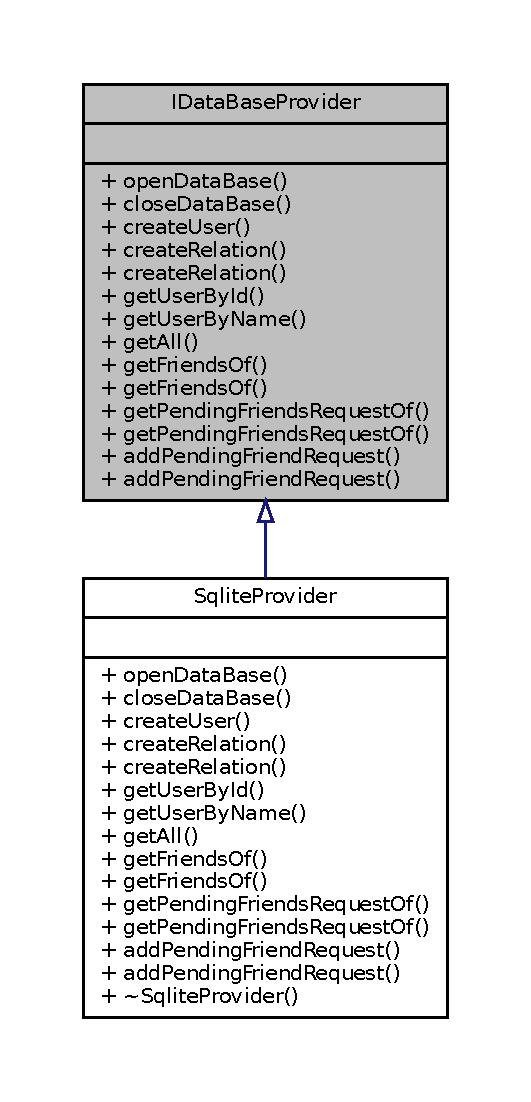
\includegraphics[width=255pt]{classIDataBaseProvider__inherit__graph}
\end{center}
\end{figure}


Collaboration diagram for I\+Data\+Base\+Provider\+:
\nopagebreak
\begin{figure}[H]
\begin{center}
\leavevmode
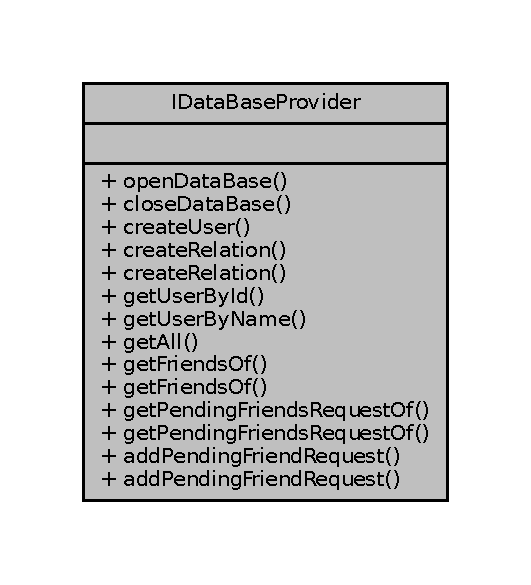
\includegraphics[width=255pt]{classIDataBaseProvider__coll__graph}
\end{center}
\end{figure}
\subsection*{Public Member Functions}
\begin{DoxyCompactItemize}
\item 
virtual bool \mbox{\hyperlink{classIDataBaseProvider_a3b467ba6923af62a82475a2a817eb1c8}{open\+Data\+Base}} (const std\+::string \&name)=0
\item 
virtual bool \mbox{\hyperlink{classIDataBaseProvider_aa7761525c25b0791d58de2429a0892ce}{close\+Data\+Base}} ()=0
\item 
virtual bool \mbox{\hyperlink{classIDataBaseProvider_ae959ea126a1fc1df9ffe058d5a3d9851}{create\+User}} (const std\+::string \&username, const std\+::string \&password)=0
\item 
virtual bool \mbox{\hyperlink{classIDataBaseProvider_adb9f20d5c7f73566b279c8564905429d}{create\+Relation}} (int a, int b)=0
\item 
virtual bool \mbox{\hyperlink{classIDataBaseProvider_ade3438db196aed2c67268f09a1b4a266}{create\+Relation}} (const std\+::string \&username1, const std\+::string \&username2)=0
\item 
virtual \mbox{\hyperlink{structUser}{User}} \mbox{\hyperlink{classIDataBaseProvider_a91cd76a2802e4dc03184f305a6624124}{get\+User\+By\+Id}} (int id)=0
\item 
virtual \mbox{\hyperlink{structUser}{User}} \mbox{\hyperlink{classIDataBaseProvider_a716a0f86654a2fbee3f4e25e2083f7cb}{get\+User\+By\+Name}} (const std\+::string \&username)=0
\item 
virtual std\+::vector$<$ \mbox{\hyperlink{structUser}{User}} $>$ \mbox{\hyperlink{classIDataBaseProvider_a15a6d47baac2391f17d911f73e68bd0f}{get\+All}} ()=0
\item 
virtual std\+::vector$<$ \mbox{\hyperlink{structUser}{User}} $>$ \mbox{\hyperlink{classIDataBaseProvider_a4d9f2f45058852ecc5cec9c949825529}{get\+Friends\+Of}} (int id)=0
\item 
virtual std\+::vector$<$ \mbox{\hyperlink{structUser}{User}} $>$ \mbox{\hyperlink{classIDataBaseProvider_a75f39a7b7596d952c0890dd5b3549569}{get\+Friends\+Of}} (const std\+::string \&username)=0
\item 
virtual std\+::vector$<$ \mbox{\hyperlink{structPendingFriendRequest}{Pending\+Friend\+Request}} $>$ \mbox{\hyperlink{classIDataBaseProvider_ad30f529c809222d72f94d15de95d44b2}{get\+Pending\+Friends\+Request\+Of}} (int id)=0
\item 
virtual std\+::vector$<$ \mbox{\hyperlink{structPendingFriendRequest}{Pending\+Friend\+Request}} $>$ \mbox{\hyperlink{classIDataBaseProvider_a376d53c78f3e101b9c0e4540330cce5b}{get\+Pending\+Friends\+Request\+Of}} (const std\+::string \&username)=0
\item 
virtual bool \mbox{\hyperlink{classIDataBaseProvider_ab8e4c2a8bb221a594947ec6216b80f95}{add\+Pending\+Friend\+Request}} (int sender, int receiver)=0
\item 
virtual bool \mbox{\hyperlink{classIDataBaseProvider_ae41b4c95e8f56e613e5e37b3563ef1f0}{add\+Pending\+Friend\+Request}} (const std\+::string \&sender, const std\+::string \&receiver)=0
\end{DoxyCompactItemize}


\subsection{Member Function Documentation}
\mbox{\Hypertarget{classIDataBaseProvider_ab8e4c2a8bb221a594947ec6216b80f95}\label{classIDataBaseProvider_ab8e4c2a8bb221a594947ec6216b80f95}} 
\index{I\+Data\+Base\+Provider@{I\+Data\+Base\+Provider}!add\+Pending\+Friend\+Request@{add\+Pending\+Friend\+Request}}
\index{add\+Pending\+Friend\+Request@{add\+Pending\+Friend\+Request}!I\+Data\+Base\+Provider@{I\+Data\+Base\+Provider}}
\subsubsection{\texorpdfstring{add\+Pending\+Friend\+Request()}{addPendingFriendRequest()}\hspace{0.1cm}{\footnotesize\ttfamily [1/2]}}
{\footnotesize\ttfamily virtual bool I\+Data\+Base\+Provider\+::add\+Pending\+Friend\+Request (\begin{DoxyParamCaption}\item[{int}]{sender,  }\item[{int}]{receiver }\end{DoxyParamCaption})\hspace{0.3cm}{\ttfamily [pure virtual]}}



Implemented in \mbox{\hyperlink{classSqliteProvider_a085e35f6de7248f7142a8e6841ab3b65}{Sqlite\+Provider}}.

\mbox{\Hypertarget{classIDataBaseProvider_ae41b4c95e8f56e613e5e37b3563ef1f0}\label{classIDataBaseProvider_ae41b4c95e8f56e613e5e37b3563ef1f0}} 
\index{I\+Data\+Base\+Provider@{I\+Data\+Base\+Provider}!add\+Pending\+Friend\+Request@{add\+Pending\+Friend\+Request}}
\index{add\+Pending\+Friend\+Request@{add\+Pending\+Friend\+Request}!I\+Data\+Base\+Provider@{I\+Data\+Base\+Provider}}
\subsubsection{\texorpdfstring{add\+Pending\+Friend\+Request()}{addPendingFriendRequest()}\hspace{0.1cm}{\footnotesize\ttfamily [2/2]}}
{\footnotesize\ttfamily virtual bool I\+Data\+Base\+Provider\+::add\+Pending\+Friend\+Request (\begin{DoxyParamCaption}\item[{const std\+::string \&}]{sender,  }\item[{const std\+::string \&}]{receiver }\end{DoxyParamCaption})\hspace{0.3cm}{\ttfamily [pure virtual]}}



Implemented in \mbox{\hyperlink{classSqliteProvider_aac8f8614546a2c5e629ad84a3536adc8}{Sqlite\+Provider}}.

\mbox{\Hypertarget{classIDataBaseProvider_aa7761525c25b0791d58de2429a0892ce}\label{classIDataBaseProvider_aa7761525c25b0791d58de2429a0892ce}} 
\index{I\+Data\+Base\+Provider@{I\+Data\+Base\+Provider}!close\+Data\+Base@{close\+Data\+Base}}
\index{close\+Data\+Base@{close\+Data\+Base}!I\+Data\+Base\+Provider@{I\+Data\+Base\+Provider}}
\subsubsection{\texorpdfstring{close\+Data\+Base()}{closeDataBase()}}
{\footnotesize\ttfamily virtual bool I\+Data\+Base\+Provider\+::close\+Data\+Base (\begin{DoxyParamCaption}{ }\end{DoxyParamCaption})\hspace{0.3cm}{\ttfamily [pure virtual]}}



Implemented in \mbox{\hyperlink{classSqliteProvider_a3f54f53f319d3c9b8c5bec57f2708c07}{Sqlite\+Provider}}.

\mbox{\Hypertarget{classIDataBaseProvider_adb9f20d5c7f73566b279c8564905429d}\label{classIDataBaseProvider_adb9f20d5c7f73566b279c8564905429d}} 
\index{I\+Data\+Base\+Provider@{I\+Data\+Base\+Provider}!create\+Relation@{create\+Relation}}
\index{create\+Relation@{create\+Relation}!I\+Data\+Base\+Provider@{I\+Data\+Base\+Provider}}
\subsubsection{\texorpdfstring{create\+Relation()}{createRelation()}\hspace{0.1cm}{\footnotesize\ttfamily [1/2]}}
{\footnotesize\ttfamily virtual bool I\+Data\+Base\+Provider\+::create\+Relation (\begin{DoxyParamCaption}\item[{int}]{a,  }\item[{int}]{b }\end{DoxyParamCaption})\hspace{0.3cm}{\ttfamily [pure virtual]}}



Implemented in \mbox{\hyperlink{classSqliteProvider_a6dc02301bf2f012306eeed7e867cec08}{Sqlite\+Provider}}.

\mbox{\Hypertarget{classIDataBaseProvider_ade3438db196aed2c67268f09a1b4a266}\label{classIDataBaseProvider_ade3438db196aed2c67268f09a1b4a266}} 
\index{I\+Data\+Base\+Provider@{I\+Data\+Base\+Provider}!create\+Relation@{create\+Relation}}
\index{create\+Relation@{create\+Relation}!I\+Data\+Base\+Provider@{I\+Data\+Base\+Provider}}
\subsubsection{\texorpdfstring{create\+Relation()}{createRelation()}\hspace{0.1cm}{\footnotesize\ttfamily [2/2]}}
{\footnotesize\ttfamily virtual bool I\+Data\+Base\+Provider\+::create\+Relation (\begin{DoxyParamCaption}\item[{const std\+::string \&}]{username1,  }\item[{const std\+::string \&}]{username2 }\end{DoxyParamCaption})\hspace{0.3cm}{\ttfamily [pure virtual]}}



Implemented in \mbox{\hyperlink{classSqliteProvider_a452f16560299d7e5f9c3f738cba13172}{Sqlite\+Provider}}.

\mbox{\Hypertarget{classIDataBaseProvider_ae959ea126a1fc1df9ffe058d5a3d9851}\label{classIDataBaseProvider_ae959ea126a1fc1df9ffe058d5a3d9851}} 
\index{I\+Data\+Base\+Provider@{I\+Data\+Base\+Provider}!create\+User@{create\+User}}
\index{create\+User@{create\+User}!I\+Data\+Base\+Provider@{I\+Data\+Base\+Provider}}
\subsubsection{\texorpdfstring{create\+User()}{createUser()}}
{\footnotesize\ttfamily virtual bool I\+Data\+Base\+Provider\+::create\+User (\begin{DoxyParamCaption}\item[{const std\+::string \&}]{username,  }\item[{const std\+::string \&}]{password }\end{DoxyParamCaption})\hspace{0.3cm}{\ttfamily [pure virtual]}}



Implemented in \mbox{\hyperlink{classSqliteProvider_a7483b0b7156adba736b6b27f8b1826a0}{Sqlite\+Provider}}.

\mbox{\Hypertarget{classIDataBaseProvider_a15a6d47baac2391f17d911f73e68bd0f}\label{classIDataBaseProvider_a15a6d47baac2391f17d911f73e68bd0f}} 
\index{I\+Data\+Base\+Provider@{I\+Data\+Base\+Provider}!get\+All@{get\+All}}
\index{get\+All@{get\+All}!I\+Data\+Base\+Provider@{I\+Data\+Base\+Provider}}
\subsubsection{\texorpdfstring{get\+All()}{getAll()}}
{\footnotesize\ttfamily virtual std\+::vector$<$\mbox{\hyperlink{structUser}{User}}$>$ I\+Data\+Base\+Provider\+::get\+All (\begin{DoxyParamCaption}{ }\end{DoxyParamCaption})\hspace{0.3cm}{\ttfamily [pure virtual]}}



Implemented in \mbox{\hyperlink{classSqliteProvider_a0b9c9b002caa7e43ed4590a6a1023525}{Sqlite\+Provider}}.

\mbox{\Hypertarget{classIDataBaseProvider_a4d9f2f45058852ecc5cec9c949825529}\label{classIDataBaseProvider_a4d9f2f45058852ecc5cec9c949825529}} 
\index{I\+Data\+Base\+Provider@{I\+Data\+Base\+Provider}!get\+Friends\+Of@{get\+Friends\+Of}}
\index{get\+Friends\+Of@{get\+Friends\+Of}!I\+Data\+Base\+Provider@{I\+Data\+Base\+Provider}}
\subsubsection{\texorpdfstring{get\+Friends\+Of()}{getFriendsOf()}\hspace{0.1cm}{\footnotesize\ttfamily [1/2]}}
{\footnotesize\ttfamily virtual std\+::vector$<$\mbox{\hyperlink{structUser}{User}}$>$ I\+Data\+Base\+Provider\+::get\+Friends\+Of (\begin{DoxyParamCaption}\item[{int}]{id }\end{DoxyParamCaption})\hspace{0.3cm}{\ttfamily [pure virtual]}}



Implemented in \mbox{\hyperlink{classSqliteProvider_a639fb7f9341b668d17917711fc5ae39a}{Sqlite\+Provider}}.

\mbox{\Hypertarget{classIDataBaseProvider_a75f39a7b7596d952c0890dd5b3549569}\label{classIDataBaseProvider_a75f39a7b7596d952c0890dd5b3549569}} 
\index{I\+Data\+Base\+Provider@{I\+Data\+Base\+Provider}!get\+Friends\+Of@{get\+Friends\+Of}}
\index{get\+Friends\+Of@{get\+Friends\+Of}!I\+Data\+Base\+Provider@{I\+Data\+Base\+Provider}}
\subsubsection{\texorpdfstring{get\+Friends\+Of()}{getFriendsOf()}\hspace{0.1cm}{\footnotesize\ttfamily [2/2]}}
{\footnotesize\ttfamily virtual std\+::vector$<$\mbox{\hyperlink{structUser}{User}}$>$ I\+Data\+Base\+Provider\+::get\+Friends\+Of (\begin{DoxyParamCaption}\item[{const std\+::string \&}]{username }\end{DoxyParamCaption})\hspace{0.3cm}{\ttfamily [pure virtual]}}



Implemented in \mbox{\hyperlink{classSqliteProvider_a19b97c70f002b84aa6a41d2d2dc9c44d}{Sqlite\+Provider}}.

\mbox{\Hypertarget{classIDataBaseProvider_ad30f529c809222d72f94d15de95d44b2}\label{classIDataBaseProvider_ad30f529c809222d72f94d15de95d44b2}} 
\index{I\+Data\+Base\+Provider@{I\+Data\+Base\+Provider}!get\+Pending\+Friends\+Request\+Of@{get\+Pending\+Friends\+Request\+Of}}
\index{get\+Pending\+Friends\+Request\+Of@{get\+Pending\+Friends\+Request\+Of}!I\+Data\+Base\+Provider@{I\+Data\+Base\+Provider}}
\subsubsection{\texorpdfstring{get\+Pending\+Friends\+Request\+Of()}{getPendingFriendsRequestOf()}\hspace{0.1cm}{\footnotesize\ttfamily [1/2]}}
{\footnotesize\ttfamily virtual std\+::vector$<$\mbox{\hyperlink{structPendingFriendRequest}{Pending\+Friend\+Request}}$>$ I\+Data\+Base\+Provider\+::get\+Pending\+Friends\+Request\+Of (\begin{DoxyParamCaption}\item[{int}]{id }\end{DoxyParamCaption})\hspace{0.3cm}{\ttfamily [pure virtual]}}



Implemented in \mbox{\hyperlink{classSqliteProvider_a199db7e0313f5e485fcf67d5a9864233}{Sqlite\+Provider}}.

\mbox{\Hypertarget{classIDataBaseProvider_a376d53c78f3e101b9c0e4540330cce5b}\label{classIDataBaseProvider_a376d53c78f3e101b9c0e4540330cce5b}} 
\index{I\+Data\+Base\+Provider@{I\+Data\+Base\+Provider}!get\+Pending\+Friends\+Request\+Of@{get\+Pending\+Friends\+Request\+Of}}
\index{get\+Pending\+Friends\+Request\+Of@{get\+Pending\+Friends\+Request\+Of}!I\+Data\+Base\+Provider@{I\+Data\+Base\+Provider}}
\subsubsection{\texorpdfstring{get\+Pending\+Friends\+Request\+Of()}{getPendingFriendsRequestOf()}\hspace{0.1cm}{\footnotesize\ttfamily [2/2]}}
{\footnotesize\ttfamily virtual std\+::vector$<$\mbox{\hyperlink{structPendingFriendRequest}{Pending\+Friend\+Request}}$>$ I\+Data\+Base\+Provider\+::get\+Pending\+Friends\+Request\+Of (\begin{DoxyParamCaption}\item[{const std\+::string \&}]{username }\end{DoxyParamCaption})\hspace{0.3cm}{\ttfamily [pure virtual]}}



Implemented in \mbox{\hyperlink{classSqliteProvider_a82dcdc27e96ff8bfe63989af3e6eff62}{Sqlite\+Provider}}.

\mbox{\Hypertarget{classIDataBaseProvider_a91cd76a2802e4dc03184f305a6624124}\label{classIDataBaseProvider_a91cd76a2802e4dc03184f305a6624124}} 
\index{I\+Data\+Base\+Provider@{I\+Data\+Base\+Provider}!get\+User\+By\+Id@{get\+User\+By\+Id}}
\index{get\+User\+By\+Id@{get\+User\+By\+Id}!I\+Data\+Base\+Provider@{I\+Data\+Base\+Provider}}
\subsubsection{\texorpdfstring{get\+User\+By\+Id()}{getUserById()}}
{\footnotesize\ttfamily virtual \mbox{\hyperlink{structUser}{User}} I\+Data\+Base\+Provider\+::get\+User\+By\+Id (\begin{DoxyParamCaption}\item[{int}]{id }\end{DoxyParamCaption})\hspace{0.3cm}{\ttfamily [pure virtual]}}



Implemented in \mbox{\hyperlink{classSqliteProvider_a1e6db27d238aadcb5871c278521aea72}{Sqlite\+Provider}}.

\mbox{\Hypertarget{classIDataBaseProvider_a716a0f86654a2fbee3f4e25e2083f7cb}\label{classIDataBaseProvider_a716a0f86654a2fbee3f4e25e2083f7cb}} 
\index{I\+Data\+Base\+Provider@{I\+Data\+Base\+Provider}!get\+User\+By\+Name@{get\+User\+By\+Name}}
\index{get\+User\+By\+Name@{get\+User\+By\+Name}!I\+Data\+Base\+Provider@{I\+Data\+Base\+Provider}}
\subsubsection{\texorpdfstring{get\+User\+By\+Name()}{getUserByName()}}
{\footnotesize\ttfamily virtual \mbox{\hyperlink{structUser}{User}} I\+Data\+Base\+Provider\+::get\+User\+By\+Name (\begin{DoxyParamCaption}\item[{const std\+::string \&}]{username }\end{DoxyParamCaption})\hspace{0.3cm}{\ttfamily [pure virtual]}}



Implemented in \mbox{\hyperlink{classSqliteProvider_a2654aee827789cfc1d40e9992d441056}{Sqlite\+Provider}}.

\mbox{\Hypertarget{classIDataBaseProvider_a3b467ba6923af62a82475a2a817eb1c8}\label{classIDataBaseProvider_a3b467ba6923af62a82475a2a817eb1c8}} 
\index{I\+Data\+Base\+Provider@{I\+Data\+Base\+Provider}!open\+Data\+Base@{open\+Data\+Base}}
\index{open\+Data\+Base@{open\+Data\+Base}!I\+Data\+Base\+Provider@{I\+Data\+Base\+Provider}}
\subsubsection{\texorpdfstring{open\+Data\+Base()}{openDataBase()}}
{\footnotesize\ttfamily virtual bool I\+Data\+Base\+Provider\+::open\+Data\+Base (\begin{DoxyParamCaption}\item[{const std\+::string \&}]{name }\end{DoxyParamCaption})\hspace{0.3cm}{\ttfamily [pure virtual]}}



Implemented in \mbox{\hyperlink{classSqliteProvider_ac37c4f4cb4438b309f7b57eda4579b79}{Sqlite\+Provider}}.



The documentation for this class was generated from the following file\+:\begin{DoxyCompactItemize}
\item 
database/\mbox{\hyperlink{IDataBaseProvider_8hpp}{I\+Data\+Base\+Provider.\+hpp}}\end{DoxyCompactItemize}

\hypertarget{classIListener}{}\section{I\+Listener Class Reference}
\label{classIListener}\index{I\+Listener@{I\+Listener}}


{\ttfamily \#include $<$I\+Listener.\+hpp$>$}



Inheritance diagram for I\+Listener\+:
\nopagebreak
\begin{figure}[H]
\begin{center}
\leavevmode
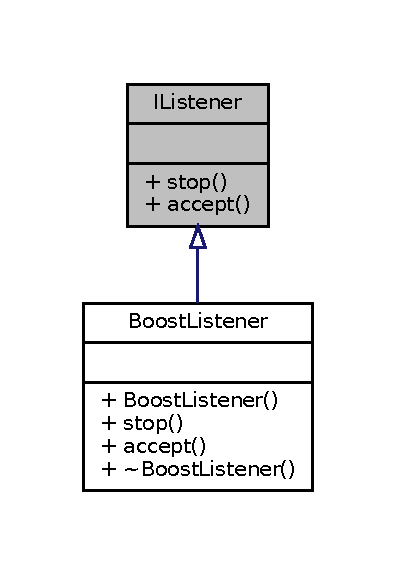
\includegraphics[width=190pt]{classIListener__inherit__graph}
\end{center}
\end{figure}


Collaboration diagram for I\+Listener\+:
\nopagebreak
\begin{figure}[H]
\begin{center}
\leavevmode
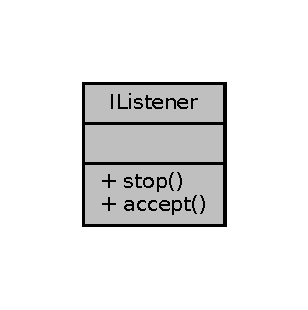
\includegraphics[width=148pt]{classIListener__coll__graph}
\end{center}
\end{figure}
\subsection*{Public Member Functions}
\begin{DoxyCompactItemize}
\item 
virtual void \mbox{\hyperlink{classIListener_a288f3ad930bc90086f4e8b6578609366}{stop}} ()=0
\item 
virtual void \mbox{\hyperlink{classIListener_a332f291fb10f7dadc223fe6c9a98a7cc}{accept}} ()=0
\end{DoxyCompactItemize}


\subsection{Member Function Documentation}
\mbox{\Hypertarget{classIListener_a332f291fb10f7dadc223fe6c9a98a7cc}\label{classIListener_a332f291fb10f7dadc223fe6c9a98a7cc}} 
\index{I\+Listener@{I\+Listener}!accept@{accept}}
\index{accept@{accept}!I\+Listener@{I\+Listener}}
\subsubsection{\texorpdfstring{accept()}{accept()}}
{\footnotesize\ttfamily virtual void I\+Listener\+::accept (\begin{DoxyParamCaption}{ }\end{DoxyParamCaption})\hspace{0.3cm}{\ttfamily [pure virtual]}}



Implemented in \mbox{\hyperlink{classBoostListener_a8a2849f0e1c513750bc74cb9a2c0d428}{Boost\+Listener}}.

\mbox{\Hypertarget{classIListener_a288f3ad930bc90086f4e8b6578609366}\label{classIListener_a288f3ad930bc90086f4e8b6578609366}} 
\index{I\+Listener@{I\+Listener}!stop@{stop}}
\index{stop@{stop}!I\+Listener@{I\+Listener}}
\subsubsection{\texorpdfstring{stop()}{stop()}}
{\footnotesize\ttfamily virtual void I\+Listener\+::stop (\begin{DoxyParamCaption}{ }\end{DoxyParamCaption})\hspace{0.3cm}{\ttfamily [pure virtual]}}



Implemented in \mbox{\hyperlink{classBoostListener_af83620fe2b6644903a6f631b8df2fd2d}{Boost\+Listener}}.



The documentation for this class was generated from the following file\+:\begin{DoxyCompactItemize}
\item 
network/\mbox{\hyperlink{IListener_8hpp}{I\+Listener.\+hpp}}\end{DoxyCompactItemize}

\hypertarget{classIService}{}\section{I\+Service Class Reference}
\label{classIService}\index{I\+Service@{I\+Service}}


{\ttfamily \#include $<$I\+Service.\+hpp$>$}



Inheritance diagram for I\+Service\+:
\nopagebreak
\begin{figure}[H]
\begin{center}
\leavevmode
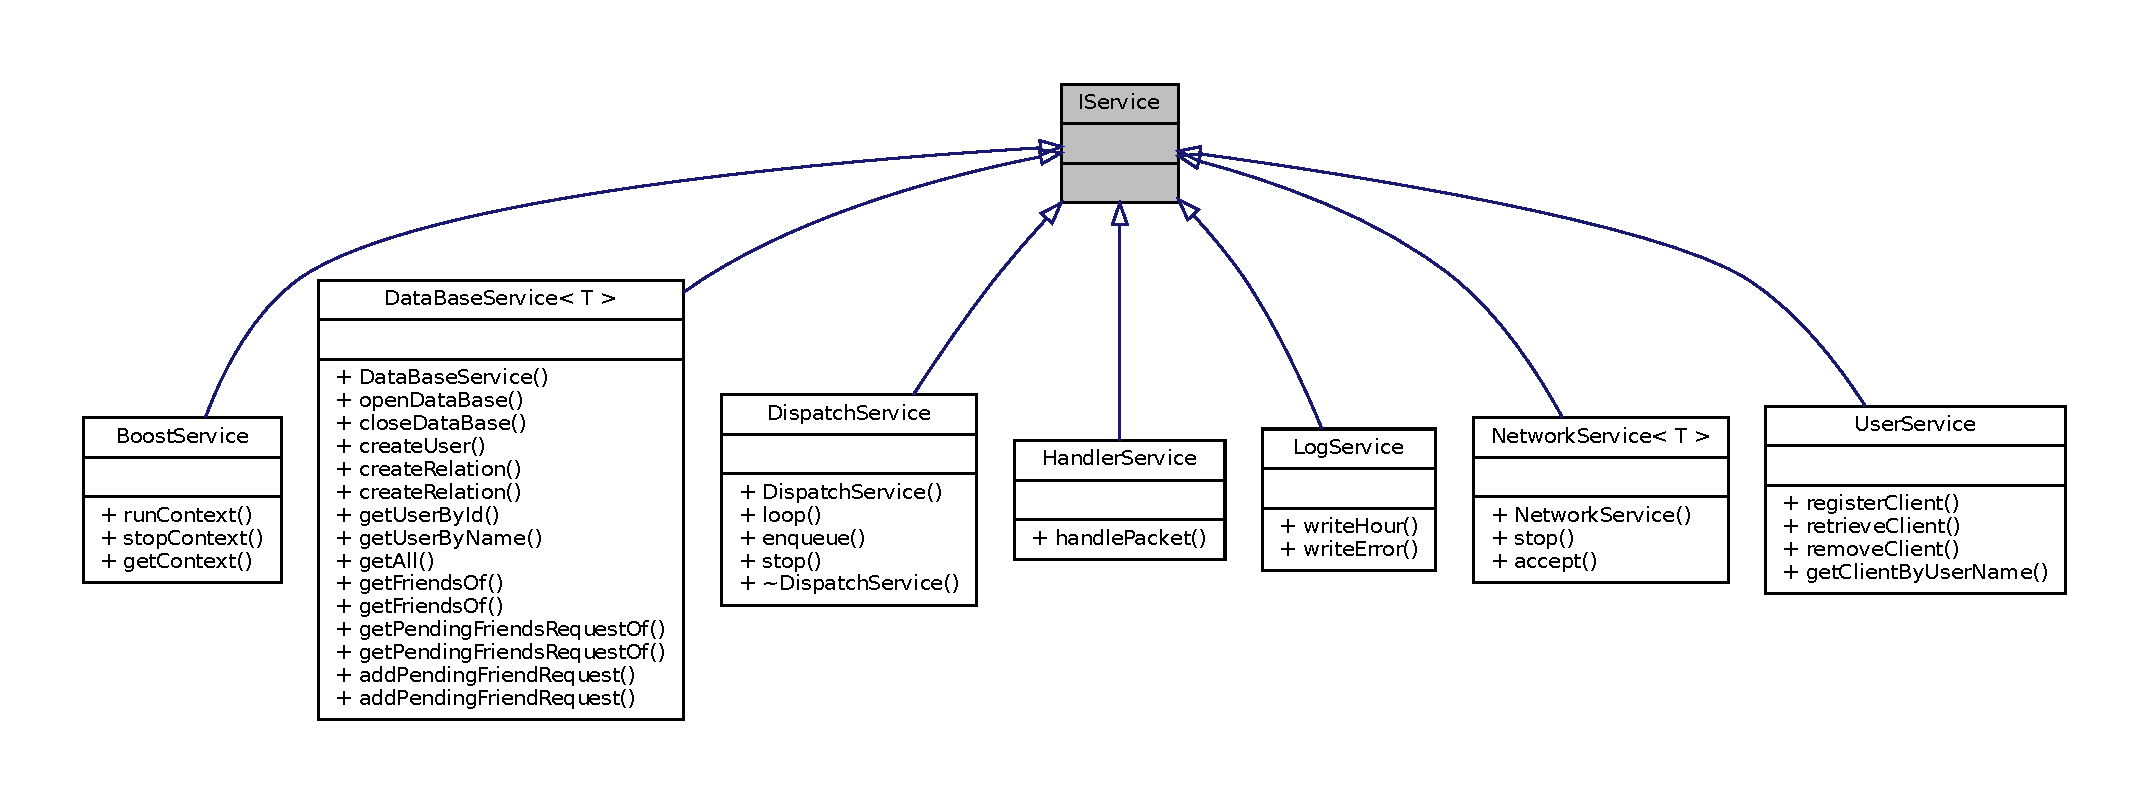
\includegraphics[width=350pt]{classIService__inherit__graph}
\end{center}
\end{figure}


Collaboration diagram for I\+Service\+:
\nopagebreak
\begin{figure}[H]
\begin{center}
\leavevmode
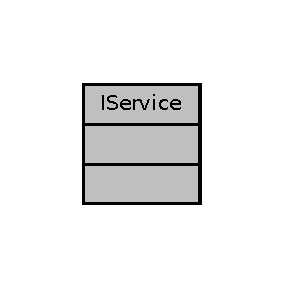
\includegraphics[width=136pt]{classIService__coll__graph}
\end{center}
\end{figure}


The documentation for this class was generated from the following file\+:\begin{DoxyCompactItemize}
\item 
services/\mbox{\hyperlink{IService_8hpp}{I\+Service.\+hpp}}\end{DoxyCompactItemize}

\hypertarget{classLogService}{}\section{Log\+Service Class Reference}
\label{classLogService}\index{Log\+Service@{Log\+Service}}


{\ttfamily \#include $<$Log\+Service.\+hpp$>$}



Inheritance diagram for Log\+Service\+:
\nopagebreak
\begin{figure}[H]
\begin{center}
\leavevmode
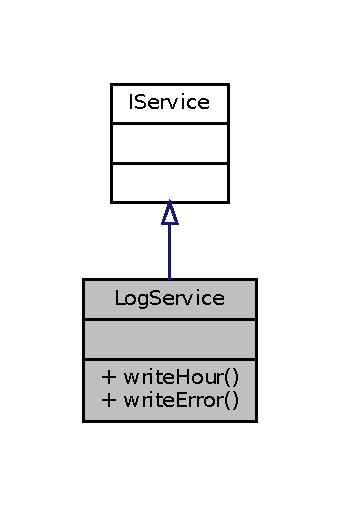
\includegraphics[width=163pt]{classLogService__inherit__graph}
\end{center}
\end{figure}


Collaboration diagram for Log\+Service\+:
\nopagebreak
\begin{figure}[H]
\begin{center}
\leavevmode
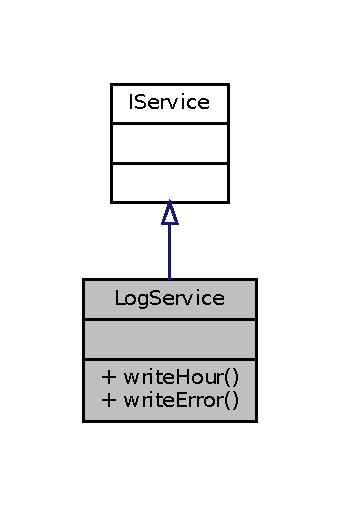
\includegraphics[width=163pt]{classLogService__coll__graph}
\end{center}
\end{figure}
\subsection*{Public Member Functions}
\begin{DoxyCompactItemize}
\item 
void \mbox{\hyperlink{classLogService_a887c03cf21e388b6951bd10c2bc234e5}{write\+Hour}} (std\+::string message)
\item 
void \mbox{\hyperlink{classLogService_a3c84c2c99960d5ec2087390cfea576d6}{write\+Error}} (std\+::string message)
\end{DoxyCompactItemize}


\subsection{Member Function Documentation}
\mbox{\Hypertarget{classLogService_a3c84c2c99960d5ec2087390cfea576d6}\label{classLogService_a3c84c2c99960d5ec2087390cfea576d6}} 
\index{Log\+Service@{Log\+Service}!write\+Error@{write\+Error}}
\index{write\+Error@{write\+Error}!Log\+Service@{Log\+Service}}
\subsubsection{\texorpdfstring{write\+Error()}{writeError()}}
{\footnotesize\ttfamily void Log\+Service\+::write\+Error (\begin{DoxyParamCaption}\item[{std\+::string}]{message }\end{DoxyParamCaption})\hspace{0.3cm}{\ttfamily [inline]}}

Here is the call graph for this function\+:
\nopagebreak
\begin{figure}[H]
\begin{center}
\leavevmode
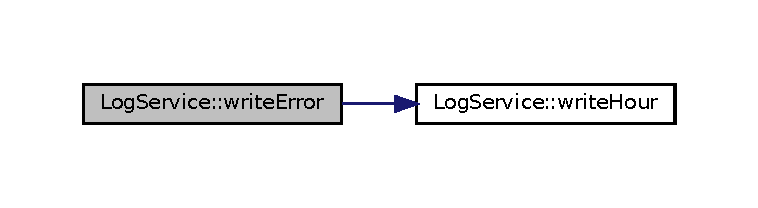
\includegraphics[width=350pt]{classLogService_a3c84c2c99960d5ec2087390cfea576d6_cgraph}
\end{center}
\end{figure}
\mbox{\Hypertarget{classLogService_a887c03cf21e388b6951bd10c2bc234e5}\label{classLogService_a887c03cf21e388b6951bd10c2bc234e5}} 
\index{Log\+Service@{Log\+Service}!write\+Hour@{write\+Hour}}
\index{write\+Hour@{write\+Hour}!Log\+Service@{Log\+Service}}
\subsubsection{\texorpdfstring{write\+Hour()}{writeHour()}}
{\footnotesize\ttfamily void Log\+Service\+::write\+Hour (\begin{DoxyParamCaption}\item[{std\+::string}]{message }\end{DoxyParamCaption})\hspace{0.3cm}{\ttfamily [inline]}}



The documentation for this class was generated from the following file\+:\begin{DoxyCompactItemize}
\item 
services/\mbox{\hyperlink{LogService_8hpp}{Log\+Service.\+hpp}}\end{DoxyCompactItemize}

\hypertarget{classNetworkService}{}\section{Network\+Service$<$ T $>$ Class Template Reference}
\label{classNetworkService}\index{Network\+Service$<$ T $>$@{Network\+Service$<$ T $>$}}


{\ttfamily \#include $<$Network\+Service.\+hpp$>$}



Inheritance diagram for Network\+Service$<$ T $>$\+:
\nopagebreak
\begin{figure}[H]
\begin{center}
\leavevmode
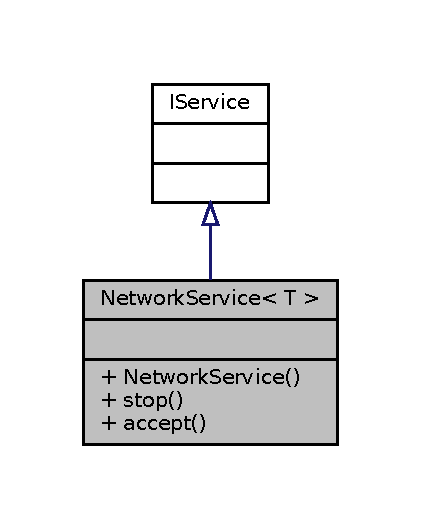
\includegraphics[width=202pt]{classNetworkService__inherit__graph}
\end{center}
\end{figure}


Collaboration diagram for Network\+Service$<$ T $>$\+:
\nopagebreak
\begin{figure}[H]
\begin{center}
\leavevmode
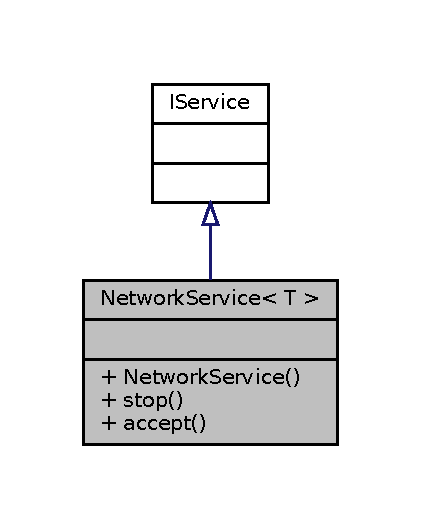
\includegraphics[width=202pt]{classNetworkService__coll__graph}
\end{center}
\end{figure}
\subsection*{Public Member Functions}
\begin{DoxyCompactItemize}
\item 
\mbox{\hyperlink{classNetworkService_ac6cdb1f63b3edc919725c5589f27cbfc}{Network\+Service}} ()
\item 
const void \mbox{\hyperlink{classNetworkService_a27bc847ca2e677729d2ca9cec06afeef}{stop}} ()
\item 
const void \mbox{\hyperlink{classNetworkService_aca54df714632e947253dc0d8184b23af}{accept}} ()
\end{DoxyCompactItemize}


\subsection{Constructor \& Destructor Documentation}
\mbox{\Hypertarget{classNetworkService_ac6cdb1f63b3edc919725c5589f27cbfc}\label{classNetworkService_ac6cdb1f63b3edc919725c5589f27cbfc}} 
\index{Network\+Service@{Network\+Service}!Network\+Service@{Network\+Service}}
\index{Network\+Service@{Network\+Service}!Network\+Service@{Network\+Service}}
\subsubsection{\texorpdfstring{Network\+Service()}{NetworkService()}}
{\footnotesize\ttfamily template$<$class T $>$ \\
\mbox{\hyperlink{classNetworkService}{Network\+Service}}$<$ T $>$\+::\mbox{\hyperlink{classNetworkService}{Network\+Service}} (\begin{DoxyParamCaption}{ }\end{DoxyParamCaption})\hspace{0.3cm}{\ttfamily [inline]}, {\ttfamily [explicit]}}



\subsection{Member Function Documentation}
\mbox{\Hypertarget{classNetworkService_aca54df714632e947253dc0d8184b23af}\label{classNetworkService_aca54df714632e947253dc0d8184b23af}} 
\index{Network\+Service@{Network\+Service}!accept@{accept}}
\index{accept@{accept}!Network\+Service@{Network\+Service}}
\subsubsection{\texorpdfstring{accept()}{accept()}}
{\footnotesize\ttfamily template$<$class T $>$ \\
const void \mbox{\hyperlink{classNetworkService}{Network\+Service}}$<$ T $>$\+::accept (\begin{DoxyParamCaption}{ }\end{DoxyParamCaption})\hspace{0.3cm}{\ttfamily [inline]}}

\mbox{\Hypertarget{classNetworkService_a27bc847ca2e677729d2ca9cec06afeef}\label{classNetworkService_a27bc847ca2e677729d2ca9cec06afeef}} 
\index{Network\+Service@{Network\+Service}!stop@{stop}}
\index{stop@{stop}!Network\+Service@{Network\+Service}}
\subsubsection{\texorpdfstring{stop()}{stop()}}
{\footnotesize\ttfamily template$<$class T $>$ \\
const void \mbox{\hyperlink{classNetworkService}{Network\+Service}}$<$ T $>$\+::stop (\begin{DoxyParamCaption}{ }\end{DoxyParamCaption})\hspace{0.3cm}{\ttfamily [inline]}}



The documentation for this class was generated from the following file\+:\begin{DoxyCompactItemize}
\item 
services/\mbox{\hyperlink{NetworkService_8hpp}{Network\+Service.\+hpp}}\end{DoxyCompactItemize}

\hypertarget{structPendingFriendRequest}{}\section{Pending\+Friend\+Request Struct Reference}
\label{structPendingFriendRequest}\index{Pending\+Friend\+Request@{Pending\+Friend\+Request}}


{\ttfamily \#include $<$Sqlite\+Provider.\+hpp$>$}



Collaboration diagram for Pending\+Friend\+Request\+:
\nopagebreak
\begin{figure}[H]
\begin{center}
\leavevmode
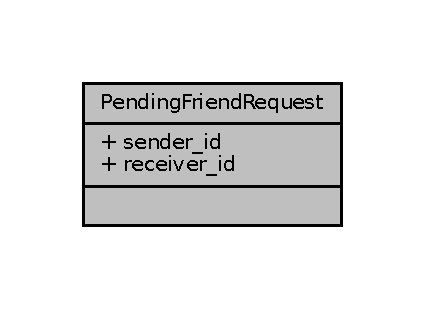
\includegraphics[width=204pt]{structPendingFriendRequest__coll__graph}
\end{center}
\end{figure}
\subsection*{Public Attributes}
\begin{DoxyCompactItemize}
\item 
int \mbox{\hyperlink{structPendingFriendRequest_a97698308250bf5be4d12079f53aed946}{sender\+\_\+id}}
\item 
int \mbox{\hyperlink{structPendingFriendRequest_a1b89fd63b19b25f6ace5ab06fbb104a3}{receiver\+\_\+id}}
\end{DoxyCompactItemize}


\subsection{Member Data Documentation}
\mbox{\Hypertarget{structPendingFriendRequest_a1b89fd63b19b25f6ace5ab06fbb104a3}\label{structPendingFriendRequest_a1b89fd63b19b25f6ace5ab06fbb104a3}} 
\index{Pending\+Friend\+Request@{Pending\+Friend\+Request}!receiver\+\_\+id@{receiver\+\_\+id}}
\index{receiver\+\_\+id@{receiver\+\_\+id}!Pending\+Friend\+Request@{Pending\+Friend\+Request}}
\subsubsection{\texorpdfstring{receiver\+\_\+id}{receiver\_id}}
{\footnotesize\ttfamily int Pending\+Friend\+Request\+::receiver\+\_\+id}

\mbox{\Hypertarget{structPendingFriendRequest_a97698308250bf5be4d12079f53aed946}\label{structPendingFriendRequest_a97698308250bf5be4d12079f53aed946}} 
\index{Pending\+Friend\+Request@{Pending\+Friend\+Request}!sender\+\_\+id@{sender\+\_\+id}}
\index{sender\+\_\+id@{sender\+\_\+id}!Pending\+Friend\+Request@{Pending\+Friend\+Request}}
\subsubsection{\texorpdfstring{sender\+\_\+id}{sender\_id}}
{\footnotesize\ttfamily int Pending\+Friend\+Request\+::sender\+\_\+id}



The documentation for this struct was generated from the following file\+:\begin{DoxyCompactItemize}
\item 
database/\mbox{\hyperlink{SqliteProvider_8hpp}{Sqlite\+Provider.\+hpp}}\end{DoxyCompactItemize}

\hypertarget{classServiceLocator}{}\section{Service\+Locator$<$ T $>$ Class Template Reference}
\label{classServiceLocator}\index{Service\+Locator$<$ T $>$@{Service\+Locator$<$ T $>$}}


{\ttfamily \#include $<$Service\+Locator.\+hpp$>$}



Collaboration diagram for Service\+Locator$<$ T $>$\+:
\nopagebreak
\begin{figure}[H]
\begin{center}
\leavevmode
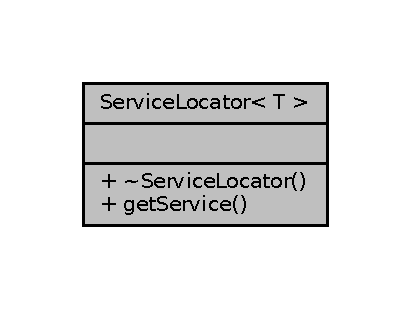
\includegraphics[width=197pt]{classServiceLocator__coll__graph}
\end{center}
\end{figure}
\subsection*{Public Member Functions}
\begin{DoxyCompactItemize}
\item 
\mbox{\hyperlink{classServiceLocator_ae001cfa8e2b3b0e7acaf1c8d95966b94}{$\sim$\+Service\+Locator}} ()
\end{DoxyCompactItemize}
\subsection*{Static Public Member Functions}
\begin{DoxyCompactItemize}
\item 
static T $\ast$ \mbox{\hyperlink{classServiceLocator_a41f5c5b0ec8ca27e1b463c5383854cbd}{get\+Service}} ()
\end{DoxyCompactItemize}


\subsection{Constructor \& Destructor Documentation}
\mbox{\Hypertarget{classServiceLocator_ae001cfa8e2b3b0e7acaf1c8d95966b94}\label{classServiceLocator_ae001cfa8e2b3b0e7acaf1c8d95966b94}} 
\index{Service\+Locator@{Service\+Locator}!````~Service\+Locator@{$\sim$\+Service\+Locator}}
\index{````~Service\+Locator@{$\sim$\+Service\+Locator}!Service\+Locator@{Service\+Locator}}
\subsubsection{\texorpdfstring{$\sim$\+Service\+Locator()}{~ServiceLocator()}}
{\footnotesize\ttfamily template$<$class T$>$ \\
\mbox{\hyperlink{classServiceLocator}{Service\+Locator}}$<$ T $>$\+::$\sim$\mbox{\hyperlink{classServiceLocator}{Service\+Locator}} (\begin{DoxyParamCaption}{ }\end{DoxyParamCaption})\hspace{0.3cm}{\ttfamily [inline]}}



\subsection{Member Function Documentation}
\mbox{\Hypertarget{classServiceLocator_a41f5c5b0ec8ca27e1b463c5383854cbd}\label{classServiceLocator_a41f5c5b0ec8ca27e1b463c5383854cbd}} 
\index{Service\+Locator@{Service\+Locator}!get\+Service@{get\+Service}}
\index{get\+Service@{get\+Service}!Service\+Locator@{Service\+Locator}}
\subsubsection{\texorpdfstring{get\+Service()}{getService()}}
{\footnotesize\ttfamily template$<$class T$>$ \\
static T$\ast$ \mbox{\hyperlink{classServiceLocator}{Service\+Locator}}$<$ T $>$\+::get\+Service (\begin{DoxyParamCaption}{ }\end{DoxyParamCaption})\hspace{0.3cm}{\ttfamily [inline]}, {\ttfamily [static]}}



The documentation for this class was generated from the following file\+:\begin{DoxyCompactItemize}
\item 
services/\mbox{\hyperlink{ServiceLocator_8hpp}{Service\+Locator.\+hpp}}\end{DoxyCompactItemize}

\hypertarget{classSqliteProvider}{}\section{Sqlite\+Provider Class Reference}
\label{classSqliteProvider}\index{Sqlite\+Provider@{Sqlite\+Provider}}


{\ttfamily \#include $<$Sqlite\+Provider.\+hpp$>$}



Inheritance diagram for Sqlite\+Provider\+:
\nopagebreak
\begin{figure}[H]
\begin{center}
\leavevmode
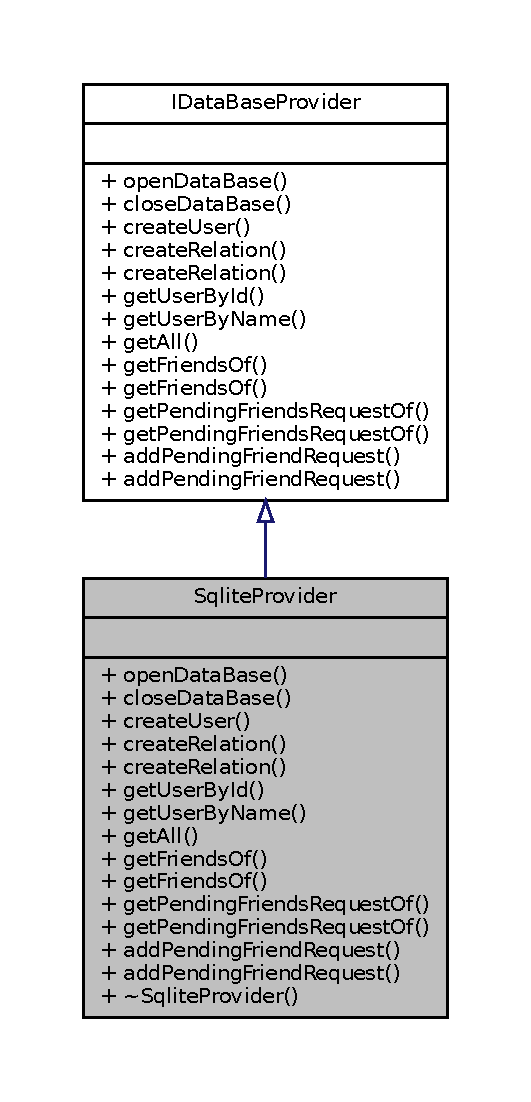
\includegraphics[width=255pt]{classSqliteProvider__inherit__graph}
\end{center}
\end{figure}


Collaboration diagram for Sqlite\+Provider\+:
\nopagebreak
\begin{figure}[H]
\begin{center}
\leavevmode
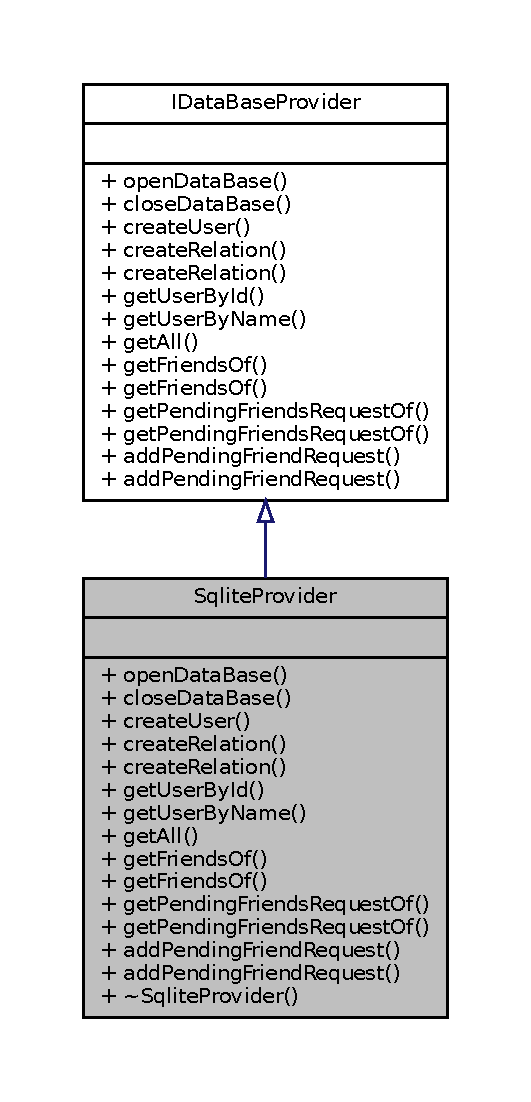
\includegraphics[width=255pt]{classSqliteProvider__coll__graph}
\end{center}
\end{figure}
\subsection*{Public Member Functions}
\begin{DoxyCompactItemize}
\item 
bool \mbox{\hyperlink{classSqliteProvider_ac37c4f4cb4438b309f7b57eda4579b79}{open\+Data\+Base}} (const std\+::string \&name) override
\item 
bool \mbox{\hyperlink{classSqliteProvider_a3f54f53f319d3c9b8c5bec57f2708c07}{close\+Data\+Base}} () override
\item 
bool \mbox{\hyperlink{classSqliteProvider_a7483b0b7156adba736b6b27f8b1826a0}{create\+User}} (const std\+::string \&username, const std\+::string \&password) override
\item 
bool \mbox{\hyperlink{classSqliteProvider_a6dc02301bf2f012306eeed7e867cec08}{create\+Relation}} (int a, int b) override
\item 
bool \mbox{\hyperlink{classSqliteProvider_a452f16560299d7e5f9c3f738cba13172}{create\+Relation}} (const std\+::string \&username1, const std\+::string \&username2) override
\item 
\mbox{\hyperlink{structUser}{User}} \mbox{\hyperlink{classSqliteProvider_a1e6db27d238aadcb5871c278521aea72}{get\+User\+By\+Id}} (int id) override
\item 
\mbox{\hyperlink{structUser}{User}} \mbox{\hyperlink{classSqliteProvider_a2654aee827789cfc1d40e9992d441056}{get\+User\+By\+Name}} (const std\+::string \&username) override
\item 
std\+::vector$<$ \mbox{\hyperlink{structUser}{User}} $>$ \mbox{\hyperlink{classSqliteProvider_a0b9c9b002caa7e43ed4590a6a1023525}{get\+All}} () override
\item 
std\+::vector$<$ \mbox{\hyperlink{structUser}{User}} $>$ \mbox{\hyperlink{classSqliteProvider_a639fb7f9341b668d17917711fc5ae39a}{get\+Friends\+Of}} (int id) override
\item 
std\+::vector$<$ \mbox{\hyperlink{structUser}{User}} $>$ \mbox{\hyperlink{classSqliteProvider_a19b97c70f002b84aa6a41d2d2dc9c44d}{get\+Friends\+Of}} (const std\+::string \&username) override
\item 
std\+::vector$<$ \mbox{\hyperlink{structPendingFriendRequest}{Pending\+Friend\+Request}} $>$ \mbox{\hyperlink{classSqliteProvider_a199db7e0313f5e485fcf67d5a9864233}{get\+Pending\+Friends\+Request\+Of}} (int id) override
\item 
std\+::vector$<$ \mbox{\hyperlink{structPendingFriendRequest}{Pending\+Friend\+Request}} $>$ \mbox{\hyperlink{classSqliteProvider_a82dcdc27e96ff8bfe63989af3e6eff62}{get\+Pending\+Friends\+Request\+Of}} (const std\+::string \&username) override
\item 
bool \mbox{\hyperlink{classSqliteProvider_a085e35f6de7248f7142a8e6841ab3b65}{add\+Pending\+Friend\+Request}} (int sender, int receiver) override
\item 
bool \mbox{\hyperlink{classSqliteProvider_aac8f8614546a2c5e629ad84a3536adc8}{add\+Pending\+Friend\+Request}} (const std\+::string \&sender, const std\+::string \&receiver) override
\item 
\mbox{\hyperlink{classSqliteProvider_a3bfff74bcbaf4f2c0eb4363fc6a07f48}{$\sim$\+Sqlite\+Provider}} ()
\end{DoxyCompactItemize}


\subsection{Constructor \& Destructor Documentation}
\mbox{\Hypertarget{classSqliteProvider_a3bfff74bcbaf4f2c0eb4363fc6a07f48}\label{classSqliteProvider_a3bfff74bcbaf4f2c0eb4363fc6a07f48}} 
\index{Sqlite\+Provider@{Sqlite\+Provider}!````~Sqlite\+Provider@{$\sim$\+Sqlite\+Provider}}
\index{````~Sqlite\+Provider@{$\sim$\+Sqlite\+Provider}!Sqlite\+Provider@{Sqlite\+Provider}}
\subsubsection{\texorpdfstring{$\sim$\+Sqlite\+Provider()}{~SqliteProvider()}}
{\footnotesize\ttfamily Sqlite\+Provider\+::$\sim$\+Sqlite\+Provider (\begin{DoxyParamCaption}{ }\end{DoxyParamCaption})\hspace{0.3cm}{\ttfamily [inline]}}

Here is the call graph for this function\+:
\nopagebreak
\begin{figure}[H]
\begin{center}
\leavevmode
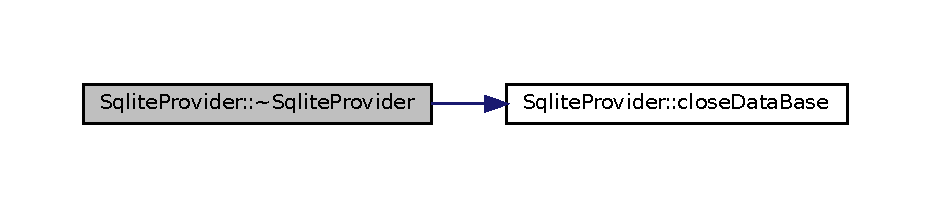
\includegraphics[width=350pt]{classSqliteProvider_a3bfff74bcbaf4f2c0eb4363fc6a07f48_cgraph}
\end{center}
\end{figure}


\subsection{Member Function Documentation}
\mbox{\Hypertarget{classSqliteProvider_a085e35f6de7248f7142a8e6841ab3b65}\label{classSqliteProvider_a085e35f6de7248f7142a8e6841ab3b65}} 
\index{Sqlite\+Provider@{Sqlite\+Provider}!add\+Pending\+Friend\+Request@{add\+Pending\+Friend\+Request}}
\index{add\+Pending\+Friend\+Request@{add\+Pending\+Friend\+Request}!Sqlite\+Provider@{Sqlite\+Provider}}
\subsubsection{\texorpdfstring{add\+Pending\+Friend\+Request()}{addPendingFriendRequest()}\hspace{0.1cm}{\footnotesize\ttfamily [1/2]}}
{\footnotesize\ttfamily bool Sqlite\+Provider\+::add\+Pending\+Friend\+Request (\begin{DoxyParamCaption}\item[{int}]{sender,  }\item[{int}]{receiver }\end{DoxyParamCaption})\hspace{0.3cm}{\ttfamily [override]}, {\ttfamily [virtual]}}



Implements \mbox{\hyperlink{classIDataBaseProvider_ab8e4c2a8bb221a594947ec6216b80f95}{I\+Data\+Base\+Provider}}.

\mbox{\Hypertarget{classSqliteProvider_aac8f8614546a2c5e629ad84a3536adc8}\label{classSqliteProvider_aac8f8614546a2c5e629ad84a3536adc8}} 
\index{Sqlite\+Provider@{Sqlite\+Provider}!add\+Pending\+Friend\+Request@{add\+Pending\+Friend\+Request}}
\index{add\+Pending\+Friend\+Request@{add\+Pending\+Friend\+Request}!Sqlite\+Provider@{Sqlite\+Provider}}
\subsubsection{\texorpdfstring{add\+Pending\+Friend\+Request()}{addPendingFriendRequest()}\hspace{0.1cm}{\footnotesize\ttfamily [2/2]}}
{\footnotesize\ttfamily bool Sqlite\+Provider\+::add\+Pending\+Friend\+Request (\begin{DoxyParamCaption}\item[{const std\+::string \&}]{sender,  }\item[{const std\+::string \&}]{receiver }\end{DoxyParamCaption})\hspace{0.3cm}{\ttfamily [override]}, {\ttfamily [virtual]}}



Implements \mbox{\hyperlink{classIDataBaseProvider_ae41b4c95e8f56e613e5e37b3563ef1f0}{I\+Data\+Base\+Provider}}.

Here is the call graph for this function\+:
\nopagebreak
\begin{figure}[H]
\begin{center}
\leavevmode
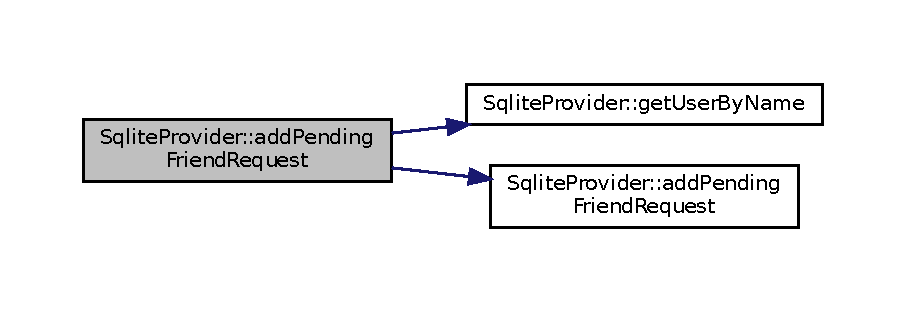
\includegraphics[width=350pt]{classSqliteProvider_aac8f8614546a2c5e629ad84a3536adc8_cgraph}
\end{center}
\end{figure}
\mbox{\Hypertarget{classSqliteProvider_a3f54f53f319d3c9b8c5bec57f2708c07}\label{classSqliteProvider_a3f54f53f319d3c9b8c5bec57f2708c07}} 
\index{Sqlite\+Provider@{Sqlite\+Provider}!close\+Data\+Base@{close\+Data\+Base}}
\index{close\+Data\+Base@{close\+Data\+Base}!Sqlite\+Provider@{Sqlite\+Provider}}
\subsubsection{\texorpdfstring{close\+Data\+Base()}{closeDataBase()}}
{\footnotesize\ttfamily bool Sqlite\+Provider\+::close\+Data\+Base (\begin{DoxyParamCaption}{ }\end{DoxyParamCaption})\hspace{0.3cm}{\ttfamily [override]}, {\ttfamily [virtual]}}



Implements \mbox{\hyperlink{classIDataBaseProvider_aa7761525c25b0791d58de2429a0892ce}{I\+Data\+Base\+Provider}}.

\mbox{\Hypertarget{classSqliteProvider_a6dc02301bf2f012306eeed7e867cec08}\label{classSqliteProvider_a6dc02301bf2f012306eeed7e867cec08}} 
\index{Sqlite\+Provider@{Sqlite\+Provider}!create\+Relation@{create\+Relation}}
\index{create\+Relation@{create\+Relation}!Sqlite\+Provider@{Sqlite\+Provider}}
\subsubsection{\texorpdfstring{create\+Relation()}{createRelation()}\hspace{0.1cm}{\footnotesize\ttfamily [1/2]}}
{\footnotesize\ttfamily bool Sqlite\+Provider\+::create\+Relation (\begin{DoxyParamCaption}\item[{int}]{a,  }\item[{int}]{b }\end{DoxyParamCaption})\hspace{0.3cm}{\ttfamily [override]}, {\ttfamily [virtual]}}



Implements \mbox{\hyperlink{classIDataBaseProvider_adb9f20d5c7f73566b279c8564905429d}{I\+Data\+Base\+Provider}}.

\mbox{\Hypertarget{classSqliteProvider_a452f16560299d7e5f9c3f738cba13172}\label{classSqliteProvider_a452f16560299d7e5f9c3f738cba13172}} 
\index{Sqlite\+Provider@{Sqlite\+Provider}!create\+Relation@{create\+Relation}}
\index{create\+Relation@{create\+Relation}!Sqlite\+Provider@{Sqlite\+Provider}}
\subsubsection{\texorpdfstring{create\+Relation()}{createRelation()}\hspace{0.1cm}{\footnotesize\ttfamily [2/2]}}
{\footnotesize\ttfamily bool Sqlite\+Provider\+::create\+Relation (\begin{DoxyParamCaption}\item[{const std\+::string \&}]{username1,  }\item[{const std\+::string \&}]{username2 }\end{DoxyParamCaption})\hspace{0.3cm}{\ttfamily [override]}, {\ttfamily [virtual]}}



Implements \mbox{\hyperlink{classIDataBaseProvider_ade3438db196aed2c67268f09a1b4a266}{I\+Data\+Base\+Provider}}.

Here is the call graph for this function\+:
\nopagebreak
\begin{figure}[H]
\begin{center}
\leavevmode
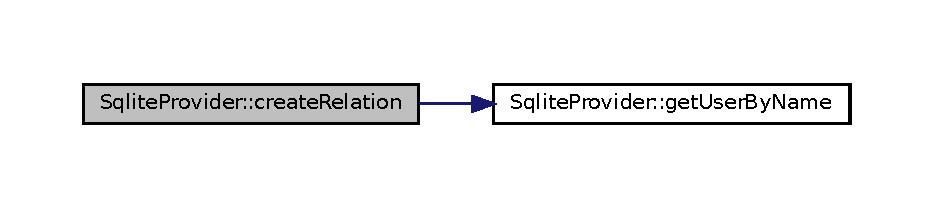
\includegraphics[width=350pt]{classSqliteProvider_a452f16560299d7e5f9c3f738cba13172_cgraph}
\end{center}
\end{figure}
\mbox{\Hypertarget{classSqliteProvider_a7483b0b7156adba736b6b27f8b1826a0}\label{classSqliteProvider_a7483b0b7156adba736b6b27f8b1826a0}} 
\index{Sqlite\+Provider@{Sqlite\+Provider}!create\+User@{create\+User}}
\index{create\+User@{create\+User}!Sqlite\+Provider@{Sqlite\+Provider}}
\subsubsection{\texorpdfstring{create\+User()}{createUser()}}
{\footnotesize\ttfamily bool Sqlite\+Provider\+::create\+User (\begin{DoxyParamCaption}\item[{const std\+::string \&}]{username,  }\item[{const std\+::string \&}]{password }\end{DoxyParamCaption})\hspace{0.3cm}{\ttfamily [override]}, {\ttfamily [virtual]}}



Implements \mbox{\hyperlink{classIDataBaseProvider_ae959ea126a1fc1df9ffe058d5a3d9851}{I\+Data\+Base\+Provider}}.

\mbox{\Hypertarget{classSqliteProvider_a0b9c9b002caa7e43ed4590a6a1023525}\label{classSqliteProvider_a0b9c9b002caa7e43ed4590a6a1023525}} 
\index{Sqlite\+Provider@{Sqlite\+Provider}!get\+All@{get\+All}}
\index{get\+All@{get\+All}!Sqlite\+Provider@{Sqlite\+Provider}}
\subsubsection{\texorpdfstring{get\+All()}{getAll()}}
{\footnotesize\ttfamily std\+::vector$<$ \mbox{\hyperlink{structUser}{User}} $>$ Sqlite\+Provider\+::get\+All (\begin{DoxyParamCaption}{ }\end{DoxyParamCaption})\hspace{0.3cm}{\ttfamily [override]}, {\ttfamily [virtual]}}



Implements \mbox{\hyperlink{classIDataBaseProvider_a15a6d47baac2391f17d911f73e68bd0f}{I\+Data\+Base\+Provider}}.

\mbox{\Hypertarget{classSqliteProvider_a639fb7f9341b668d17917711fc5ae39a}\label{classSqliteProvider_a639fb7f9341b668d17917711fc5ae39a}} 
\index{Sqlite\+Provider@{Sqlite\+Provider}!get\+Friends\+Of@{get\+Friends\+Of}}
\index{get\+Friends\+Of@{get\+Friends\+Of}!Sqlite\+Provider@{Sqlite\+Provider}}
\subsubsection{\texorpdfstring{get\+Friends\+Of()}{getFriendsOf()}\hspace{0.1cm}{\footnotesize\ttfamily [1/2]}}
{\footnotesize\ttfamily std\+::vector$<$ \mbox{\hyperlink{structUser}{User}} $>$ Sqlite\+Provider\+::get\+Friends\+Of (\begin{DoxyParamCaption}\item[{int}]{id }\end{DoxyParamCaption})\hspace{0.3cm}{\ttfamily [override]}, {\ttfamily [virtual]}}



Implements \mbox{\hyperlink{classIDataBaseProvider_a4d9f2f45058852ecc5cec9c949825529}{I\+Data\+Base\+Provider}}.

Here is the call graph for this function\+:
\nopagebreak
\begin{figure}[H]
\begin{center}
\leavevmode
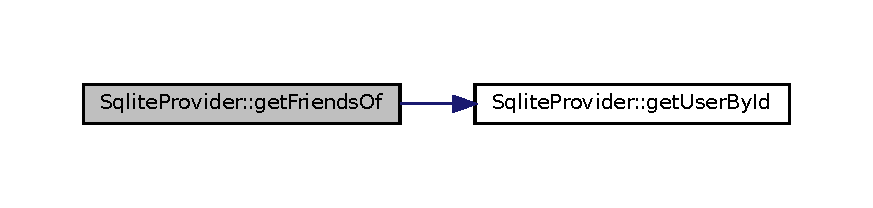
\includegraphics[width=350pt]{classSqliteProvider_a639fb7f9341b668d17917711fc5ae39a_cgraph}
\end{center}
\end{figure}
\mbox{\Hypertarget{classSqliteProvider_a19b97c70f002b84aa6a41d2d2dc9c44d}\label{classSqliteProvider_a19b97c70f002b84aa6a41d2d2dc9c44d}} 
\index{Sqlite\+Provider@{Sqlite\+Provider}!get\+Friends\+Of@{get\+Friends\+Of}}
\index{get\+Friends\+Of@{get\+Friends\+Of}!Sqlite\+Provider@{Sqlite\+Provider}}
\subsubsection{\texorpdfstring{get\+Friends\+Of()}{getFriendsOf()}\hspace{0.1cm}{\footnotesize\ttfamily [2/2]}}
{\footnotesize\ttfamily std\+::vector$<$ \mbox{\hyperlink{structUser}{User}} $>$ Sqlite\+Provider\+::get\+Friends\+Of (\begin{DoxyParamCaption}\item[{const std\+::string \&}]{username }\end{DoxyParamCaption})\hspace{0.3cm}{\ttfamily [override]}, {\ttfamily [virtual]}}



Implements \mbox{\hyperlink{classIDataBaseProvider_a75f39a7b7596d952c0890dd5b3549569}{I\+Data\+Base\+Provider}}.

Here is the call graph for this function\+:
\nopagebreak
\begin{figure}[H]
\begin{center}
\leavevmode
\includegraphics[width=350pt]{classSqliteProvider_a19b97c70f002b84aa6a41d2d2dc9c44d_cgraph}
\end{center}
\end{figure}
\mbox{\Hypertarget{classSqliteProvider_a199db7e0313f5e485fcf67d5a9864233}\label{classSqliteProvider_a199db7e0313f5e485fcf67d5a9864233}} 
\index{Sqlite\+Provider@{Sqlite\+Provider}!get\+Pending\+Friends\+Request\+Of@{get\+Pending\+Friends\+Request\+Of}}
\index{get\+Pending\+Friends\+Request\+Of@{get\+Pending\+Friends\+Request\+Of}!Sqlite\+Provider@{Sqlite\+Provider}}
\subsubsection{\texorpdfstring{get\+Pending\+Friends\+Request\+Of()}{getPendingFriendsRequestOf()}\hspace{0.1cm}{\footnotesize\ttfamily [1/2]}}
{\footnotesize\ttfamily std\+::vector$<$ \mbox{\hyperlink{structPendingFriendRequest}{Pending\+Friend\+Request}} $>$ Sqlite\+Provider\+::get\+Pending\+Friends\+Request\+Of (\begin{DoxyParamCaption}\item[{int}]{id }\end{DoxyParamCaption})\hspace{0.3cm}{\ttfamily [override]}, {\ttfamily [virtual]}}



Implements \mbox{\hyperlink{classIDataBaseProvider_ad30f529c809222d72f94d15de95d44b2}{I\+Data\+Base\+Provider}}.

\mbox{\Hypertarget{classSqliteProvider_a82dcdc27e96ff8bfe63989af3e6eff62}\label{classSqliteProvider_a82dcdc27e96ff8bfe63989af3e6eff62}} 
\index{Sqlite\+Provider@{Sqlite\+Provider}!get\+Pending\+Friends\+Request\+Of@{get\+Pending\+Friends\+Request\+Of}}
\index{get\+Pending\+Friends\+Request\+Of@{get\+Pending\+Friends\+Request\+Of}!Sqlite\+Provider@{Sqlite\+Provider}}
\subsubsection{\texorpdfstring{get\+Pending\+Friends\+Request\+Of()}{getPendingFriendsRequestOf()}\hspace{0.1cm}{\footnotesize\ttfamily [2/2]}}
{\footnotesize\ttfamily std\+::vector$<$ \mbox{\hyperlink{structPendingFriendRequest}{Pending\+Friend\+Request}} $>$ Sqlite\+Provider\+::get\+Pending\+Friends\+Request\+Of (\begin{DoxyParamCaption}\item[{const std\+::string \&}]{username }\end{DoxyParamCaption})\hspace{0.3cm}{\ttfamily [override]}, {\ttfamily [virtual]}}



Implements \mbox{\hyperlink{classIDataBaseProvider_a376d53c78f3e101b9c0e4540330cce5b}{I\+Data\+Base\+Provider}}.

Here is the call graph for this function\+:
\nopagebreak
\begin{figure}[H]
\begin{center}
\leavevmode
\includegraphics[width=350pt]{classSqliteProvider_a82dcdc27e96ff8bfe63989af3e6eff62_cgraph}
\end{center}
\end{figure}
\mbox{\Hypertarget{classSqliteProvider_a1e6db27d238aadcb5871c278521aea72}\label{classSqliteProvider_a1e6db27d238aadcb5871c278521aea72}} 
\index{Sqlite\+Provider@{Sqlite\+Provider}!get\+User\+By\+Id@{get\+User\+By\+Id}}
\index{get\+User\+By\+Id@{get\+User\+By\+Id}!Sqlite\+Provider@{Sqlite\+Provider}}
\subsubsection{\texorpdfstring{get\+User\+By\+Id()}{getUserById()}}
{\footnotesize\ttfamily \mbox{\hyperlink{structUser}{User}} Sqlite\+Provider\+::get\+User\+By\+Id (\begin{DoxyParamCaption}\item[{int}]{id }\end{DoxyParamCaption})\hspace{0.3cm}{\ttfamily [override]}, {\ttfamily [virtual]}}



Implements \mbox{\hyperlink{classIDataBaseProvider_a91cd76a2802e4dc03184f305a6624124}{I\+Data\+Base\+Provider}}.

\mbox{\Hypertarget{classSqliteProvider_a2654aee827789cfc1d40e9992d441056}\label{classSqliteProvider_a2654aee827789cfc1d40e9992d441056}} 
\index{Sqlite\+Provider@{Sqlite\+Provider}!get\+User\+By\+Name@{get\+User\+By\+Name}}
\index{get\+User\+By\+Name@{get\+User\+By\+Name}!Sqlite\+Provider@{Sqlite\+Provider}}
\subsubsection{\texorpdfstring{get\+User\+By\+Name()}{getUserByName()}}
{\footnotesize\ttfamily \mbox{\hyperlink{structUser}{User}} Sqlite\+Provider\+::get\+User\+By\+Name (\begin{DoxyParamCaption}\item[{const std\+::string \&}]{username }\end{DoxyParamCaption})\hspace{0.3cm}{\ttfamily [override]}, {\ttfamily [virtual]}}



Implements \mbox{\hyperlink{classIDataBaseProvider_a716a0f86654a2fbee3f4e25e2083f7cb}{I\+Data\+Base\+Provider}}.

\mbox{\Hypertarget{classSqliteProvider_ac37c4f4cb4438b309f7b57eda4579b79}\label{classSqliteProvider_ac37c4f4cb4438b309f7b57eda4579b79}} 
\index{Sqlite\+Provider@{Sqlite\+Provider}!open\+Data\+Base@{open\+Data\+Base}}
\index{open\+Data\+Base@{open\+Data\+Base}!Sqlite\+Provider@{Sqlite\+Provider}}
\subsubsection{\texorpdfstring{open\+Data\+Base()}{openDataBase()}}
{\footnotesize\ttfamily bool Sqlite\+Provider\+::open\+Data\+Base (\begin{DoxyParamCaption}\item[{const std\+::string \&}]{name }\end{DoxyParamCaption})\hspace{0.3cm}{\ttfamily [override]}, {\ttfamily [virtual]}}



Implements \mbox{\hyperlink{classIDataBaseProvider_a3b467ba6923af62a82475a2a817eb1c8}{I\+Data\+Base\+Provider}}.

Here is the call graph for this function\+:
\nopagebreak
\begin{figure}[H]
\begin{center}
\leavevmode
\includegraphics[width=348pt]{classSqliteProvider_ac37c4f4cb4438b309f7b57eda4579b79_cgraph}
\end{center}
\end{figure}


The documentation for this class was generated from the following files\+:\begin{DoxyCompactItemize}
\item 
database/\mbox{\hyperlink{SqliteProvider_8hpp}{Sqlite\+Provider.\+hpp}}\item 
database/\mbox{\hyperlink{SqliteProvider_8cpp}{Sqlite\+Provider.\+cpp}}\end{DoxyCompactItemize}

\hypertarget{structUser}{}\section{User Struct Reference}
\label{structUser}\index{User@{User}}


{\ttfamily \#include $<$Sqlite\+Provider.\+hpp$>$}



Collaboration diagram for User\+:
\nopagebreak
\begin{figure}[H]
\begin{center}
\leavevmode
\includegraphics[width=157pt]{structUser__coll__graph}
\end{center}
\end{figure}
\subsection*{Public Attributes}
\begin{DoxyCompactItemize}
\item 
int \mbox{\hyperlink{structUser_aa7e6e39b43020bbe9c3a196b3689b0f7}{id}}
\item 
std\+::string \mbox{\hyperlink{structUser_aacbb807e514280f69e00bec7d71f3aee}{username}}
\item 
std\+::string \mbox{\hyperlink{structUser_ac2f2e75b15e8eb6cbb030fc85a6cd59f}{password}}
\end{DoxyCompactItemize}


\subsection{Member Data Documentation}
\mbox{\Hypertarget{structUser_aa7e6e39b43020bbe9c3a196b3689b0f7}\label{structUser_aa7e6e39b43020bbe9c3a196b3689b0f7}} 
\index{User@{User}!id@{id}}
\index{id@{id}!User@{User}}
\subsubsection{\texorpdfstring{id}{id}}
{\footnotesize\ttfamily int User\+::id}

\mbox{\Hypertarget{structUser_ac2f2e75b15e8eb6cbb030fc85a6cd59f}\label{structUser_ac2f2e75b15e8eb6cbb030fc85a6cd59f}} 
\index{User@{User}!password@{password}}
\index{password@{password}!User@{User}}
\subsubsection{\texorpdfstring{password}{password}}
{\footnotesize\ttfamily std\+::string User\+::password}

\mbox{\Hypertarget{structUser_aacbb807e514280f69e00bec7d71f3aee}\label{structUser_aacbb807e514280f69e00bec7d71f3aee}} 
\index{User@{User}!username@{username}}
\index{username@{username}!User@{User}}
\subsubsection{\texorpdfstring{username}{username}}
{\footnotesize\ttfamily std\+::string User\+::username}



The documentation for this struct was generated from the following file\+:\begin{DoxyCompactItemize}
\item 
database/\mbox{\hyperlink{SqliteProvider_8hpp}{Sqlite\+Provider.\+hpp}}\end{DoxyCompactItemize}

\hypertarget{classUserService}{}\section{User\+Service Class Reference}
\label{classUserService}\index{User\+Service@{User\+Service}}


{\ttfamily \#include $<$User\+Service.\+hpp$>$}



Inheritance diagram for User\+Service\+:
\nopagebreak
\begin{figure}[H]
\begin{center}
\leavevmode
\includegraphics[width=224pt]{classUserService__inherit__graph}
\end{center}
\end{figure}


Collaboration diagram for User\+Service\+:
\nopagebreak
\begin{figure}[H]
\begin{center}
\leavevmode
\includegraphics[width=224pt]{classUserService__coll__graph}
\end{center}
\end{figure}
\subsection*{Public Member Functions}
\begin{DoxyCompactItemize}
\item 
void \mbox{\hyperlink{classUserService_a7fde1ac30d6bc9e9177def82097cd73b}{register\+Client}} (boost\+::shared\+\_\+ptr$<$ \mbox{\hyperlink{classIConnection}{I\+Connection}} $>$ \&connection)
\item 
boost\+::shared\+\_\+ptr$<$ \mbox{\hyperlink{classClient}{Client}} $>$ \mbox{\hyperlink{classUserService_a2f79f2e036977fd16ae7ca14b1017530}{retrieve\+Client}} (boost\+::shared\+\_\+ptr$<$ \mbox{\hyperlink{classIConnection}{I\+Connection}} $>$ \&connection)
\item 
void \mbox{\hyperlink{classUserService_af919fd2cca398408c61081aaadb26e88}{remove\+Client}} (boost\+::shared\+\_\+ptr$<$ \mbox{\hyperlink{classIConnection}{I\+Connection}} $>$ \&connection)
\item 
boost\+::shared\+\_\+ptr$<$ \mbox{\hyperlink{classClient}{Client}} $>$ \mbox{\hyperlink{classUserService_a8eaccab3dc50dd0b69c917b906926f95}{get\+Client\+By\+User\+Name}} (const std\+::string \&username)
\end{DoxyCompactItemize}


\subsection{Member Function Documentation}
\mbox{\Hypertarget{classUserService_a8eaccab3dc50dd0b69c917b906926f95}\label{classUserService_a8eaccab3dc50dd0b69c917b906926f95}} 
\index{User\+Service@{User\+Service}!get\+Client\+By\+User\+Name@{get\+Client\+By\+User\+Name}}
\index{get\+Client\+By\+User\+Name@{get\+Client\+By\+User\+Name}!User\+Service@{User\+Service}}
\subsubsection{\texorpdfstring{get\+Client\+By\+User\+Name()}{getClientByUserName()}}
{\footnotesize\ttfamily boost\+::shared\+\_\+ptr$<$\mbox{\hyperlink{classClient}{Client}}$>$ User\+Service\+::get\+Client\+By\+User\+Name (\begin{DoxyParamCaption}\item[{const std\+::string \&}]{username }\end{DoxyParamCaption})\hspace{0.3cm}{\ttfamily [inline]}}

\mbox{\Hypertarget{classUserService_a7fde1ac30d6bc9e9177def82097cd73b}\label{classUserService_a7fde1ac30d6bc9e9177def82097cd73b}} 
\index{User\+Service@{User\+Service}!register\+Client@{register\+Client}}
\index{register\+Client@{register\+Client}!User\+Service@{User\+Service}}
\subsubsection{\texorpdfstring{register\+Client()}{registerClient()}}
{\footnotesize\ttfamily void User\+Service\+::register\+Client (\begin{DoxyParamCaption}\item[{boost\+::shared\+\_\+ptr$<$ \mbox{\hyperlink{classIConnection}{I\+Connection}} $>$ \&}]{connection }\end{DoxyParamCaption})\hspace{0.3cm}{\ttfamily [inline]}}

Here is the call graph for this function\+:
\nopagebreak
\begin{figure}[H]
\begin{center}
\leavevmode
\includegraphics[width=345pt]{classUserService_a7fde1ac30d6bc9e9177def82097cd73b_cgraph}
\end{center}
\end{figure}
\mbox{\Hypertarget{classUserService_af919fd2cca398408c61081aaadb26e88}\label{classUserService_af919fd2cca398408c61081aaadb26e88}} 
\index{User\+Service@{User\+Service}!remove\+Client@{remove\+Client}}
\index{remove\+Client@{remove\+Client}!User\+Service@{User\+Service}}
\subsubsection{\texorpdfstring{remove\+Client()}{removeClient()}}
{\footnotesize\ttfamily void User\+Service\+::remove\+Client (\begin{DoxyParamCaption}\item[{boost\+::shared\+\_\+ptr$<$ \mbox{\hyperlink{classIConnection}{I\+Connection}} $>$ \&}]{connection }\end{DoxyParamCaption})\hspace{0.3cm}{\ttfamily [inline]}}

\mbox{\Hypertarget{classUserService_a2f79f2e036977fd16ae7ca14b1017530}\label{classUserService_a2f79f2e036977fd16ae7ca14b1017530}} 
\index{User\+Service@{User\+Service}!retrieve\+Client@{retrieve\+Client}}
\index{retrieve\+Client@{retrieve\+Client}!User\+Service@{User\+Service}}
\subsubsection{\texorpdfstring{retrieve\+Client()}{retrieveClient()}}
{\footnotesize\ttfamily boost\+::shared\+\_\+ptr$<$\mbox{\hyperlink{classClient}{Client}}$>$ User\+Service\+::retrieve\+Client (\begin{DoxyParamCaption}\item[{boost\+::shared\+\_\+ptr$<$ \mbox{\hyperlink{classIConnection}{I\+Connection}} $>$ \&}]{connection }\end{DoxyParamCaption})\hspace{0.3cm}{\ttfamily [inline]}}



The documentation for this class was generated from the following file\+:\begin{DoxyCompactItemize}
\item 
services/\mbox{\hyperlink{UserService_8hpp}{User\+Service.\+hpp}}\end{DoxyCompactItemize}

\chapter{File Documentation}
\hypertarget{IDataBaseProvider_8hpp}{}\section{database/\+I\+Data\+Base\+Provider.hpp File Reference}
\label{IDataBaseProvider_8hpp}\index{database/\+I\+Data\+Base\+Provider.\+hpp@{database/\+I\+Data\+Base\+Provider.\+hpp}}
{\ttfamily \#include $<$string$>$}\newline
Include dependency graph for I\+Data\+Base\+Provider.\+hpp\+:
\nopagebreak
\begin{figure}[H]
\begin{center}
\leavevmode
\includegraphics[width=256pt]{IDataBaseProvider_8hpp__incl}
\end{center}
\end{figure}
This graph shows which files directly or indirectly include this file\+:
\nopagebreak
\begin{figure}[H]
\begin{center}
\leavevmode
\includegraphics[width=350pt]{IDataBaseProvider_8hpp__dep__incl}
\end{center}
\end{figure}
\subsection*{Classes}
\begin{DoxyCompactItemize}
\item 
class \mbox{\hyperlink{classIDataBaseProvider}{I\+Data\+Base\+Provider}}
\end{DoxyCompactItemize}

\hypertarget{SqliteProvider_8cpp}{}\section{database/\+Sqlite\+Provider.cpp File Reference}
\label{SqliteProvider_8cpp}\index{database/\+Sqlite\+Provider.\+cpp@{database/\+Sqlite\+Provider.\+cpp}}
{\ttfamily \#include $<$iostream$>$}\newline
{\ttfamily \#include $<$sqlite\+\_\+orm/sqlite\+\_\+orm.\+h$>$}\newline
{\ttfamily \#include \char`\"{}Sqlite\+Provider.\+hpp\char`\"{}}\newline
Include dependency graph for Sqlite\+Provider.\+cpp\+:
\nopagebreak
\begin{figure}[H]
\begin{center}
\leavevmode
\includegraphics[width=350pt]{SqliteProvider_8cpp__incl}
\end{center}
\end{figure}

\hypertarget{SqliteProvider_8hpp}{}\section{database/\+Sqlite\+Provider.hpp File Reference}
\label{SqliteProvider_8hpp}\index{database/\+Sqlite\+Provider.\+hpp@{database/\+Sqlite\+Provider.\+hpp}}
{\ttfamily \#include $<$string$>$}\newline
{\ttfamily \#include $<$sqlite3.\+h$>$}\newline
{\ttfamily \#include $<$functional$>$}\newline
{\ttfamily \#include $<$sqlite\+\_\+orm/sqlite\+\_\+orm.\+h$>$}\newline
{\ttfamily \#include \char`\"{}I\+Data\+Base\+Provider.\+hpp\char`\"{}}\newline
Include dependency graph for Sqlite\+Provider.\+hpp\+:
\nopagebreak
\begin{figure}[H]
\begin{center}
\leavevmode
\includegraphics[width=350pt]{SqliteProvider_8hpp__incl}
\end{center}
\end{figure}
This graph shows which files directly or indirectly include this file\+:
\nopagebreak
\begin{figure}[H]
\begin{center}
\leavevmode
\includegraphics[width=350pt]{SqliteProvider_8hpp__dep__incl}
\end{center}
\end{figure}
\subsection*{Classes}
\begin{DoxyCompactItemize}
\item 
struct \mbox{\hyperlink{structUser}{User}}
\item 
struct \mbox{\hyperlink{structFriendship}{Friendship}}
\item 
struct \mbox{\hyperlink{structPendingFriendRequest}{Pending\+Friend\+Request}}
\item 
class \mbox{\hyperlink{classSqliteProvider}{Sqlite\+Provider}}
\end{DoxyCompactItemize}
\subsection*{Typedefs}
\begin{DoxyCompactItemize}
\item 
using \mbox{\hyperlink{SqliteProvider_8hpp_acdd2f9e14560ab96d15cec4fa102b096}{Storage}} = decltype(\mbox{\hyperlink{SqliteProvider_8hpp_a6cd3bdf970d149dea73c089dc8fe1220}{init\+Storage}}(\char`\"{}\char`\"{}))
\end{DoxyCompactItemize}
\subsection*{Functions}
\begin{DoxyCompactItemize}
\item 
auto \mbox{\hyperlink{SqliteProvider_8hpp_a6cd3bdf970d149dea73c089dc8fe1220}{init\+Storage}} (const std\+::string \&name)
\end{DoxyCompactItemize}


\subsection{Typedef Documentation}
\mbox{\Hypertarget{SqliteProvider_8hpp_acdd2f9e14560ab96d15cec4fa102b096}\label{SqliteProvider_8hpp_acdd2f9e14560ab96d15cec4fa102b096}} 
\index{Sqlite\+Provider.\+hpp@{Sqlite\+Provider.\+hpp}!Storage@{Storage}}
\index{Storage@{Storage}!Sqlite\+Provider.\+hpp@{Sqlite\+Provider.\+hpp}}
\subsubsection{\texorpdfstring{Storage}{Storage}}
{\footnotesize\ttfamily using \mbox{\hyperlink{SqliteProvider_8hpp_acdd2f9e14560ab96d15cec4fa102b096}{Storage}} =  decltype(\mbox{\hyperlink{SqliteProvider_8hpp_a6cd3bdf970d149dea73c089dc8fe1220}{init\+Storage}}(\char`\"{}\char`\"{}))}



\subsection{Function Documentation}
\mbox{\Hypertarget{SqliteProvider_8hpp_a6cd3bdf970d149dea73c089dc8fe1220}\label{SqliteProvider_8hpp_a6cd3bdf970d149dea73c089dc8fe1220}} 
\index{Sqlite\+Provider.\+hpp@{Sqlite\+Provider.\+hpp}!init\+Storage@{init\+Storage}}
\index{init\+Storage@{init\+Storage}!Sqlite\+Provider.\+hpp@{Sqlite\+Provider.\+hpp}}
\subsubsection{\texorpdfstring{init\+Storage()}{initStorage()}}
{\footnotesize\ttfamily auto init\+Storage (\begin{DoxyParamCaption}\item[{const std\+::string \&}]{name }\end{DoxyParamCaption})\hspace{0.3cm}{\ttfamily [inline]}}


\hypertarget{Client_8hpp}{}\section{logic/\+Client.hpp File Reference}
\label{Client_8hpp}\index{logic/\+Client.\+hpp@{logic/\+Client.\+hpp}}
{\ttfamily \#include $<$boost/asio.\+hpp$>$}\newline
{\ttfamily \#include \char`\"{}I\+Packet.\+hpp\char`\"{}}\newline
{\ttfamily \#include \char`\"{}I\+O/\+Native\+Binary\+Writer.\+hpp\char`\"{}}\newline
{\ttfamily \#include \char`\"{}network/\+I\+Connection.\+hpp\char`\"{}}\newline
{\ttfamily \#include \char`\"{}database/\+Sqlite\+Provider.\+hpp\char`\"{}}\newline
Include dependency graph for Client.\+hpp\+:
\nopagebreak
\begin{figure}[H]
\begin{center}
\leavevmode
\includegraphics[width=350pt]{Client_8hpp__incl}
\end{center}
\end{figure}
This graph shows which files directly or indirectly include this file\+:
\nopagebreak
\begin{figure}[H]
\begin{center}
\leavevmode
\includegraphics[width=350pt]{Client_8hpp__dep__incl}
\end{center}
\end{figure}
\subsection*{Classes}
\begin{DoxyCompactItemize}
\item 
class \mbox{\hyperlink{classClient}{Client}}
\end{DoxyCompactItemize}

\hypertarget{HandshakeHandler_8cpp}{}\section{logic/handshake/\+Handshake\+Handler.cpp File Reference}
\label{HandshakeHandler_8cpp}\index{logic/handshake/\+Handshake\+Handler.\+cpp@{logic/handshake/\+Handshake\+Handler.\+cpp}}
{\ttfamily \#include $<$services/\+User\+Service.\+hpp$>$}\newline
{\ttfamily \#include \char`\"{}Handshake\+Handler.\+hpp\char`\"{}}\newline
{\ttfamily \#include \char`\"{}Packet\+Factory.\+hpp\char`\"{}}\newline
{\ttfamily \#include \char`\"{}database/\+Sqlite\+Provider.\+hpp\char`\"{}}\newline
{\ttfamily \#include \char`\"{}services/\+Service\+Locator.\+hpp\char`\"{}}\newline
{\ttfamily \#include \char`\"{}services/\+Data\+Base\+Service.\+hpp\char`\"{}}\newline
Include dependency graph for Handshake\+Handler.\+cpp\+:
\nopagebreak
\begin{figure}[H]
\begin{center}
\leavevmode
\includegraphics[width=350pt]{HandshakeHandler_8cpp__incl}
\end{center}
\end{figure}

\hypertarget{HandshakeHandler_8hpp}{}\section{logic/handshake/\+Handshake\+Handler.hpp File Reference}
\label{HandshakeHandler_8hpp}\index{logic/handshake/\+Handshake\+Handler.\+hpp@{logic/handshake/\+Handshake\+Handler.\+hpp}}
{\ttfamily \#include \char`\"{}logic/\+Client.\+hpp\char`\"{}}\newline
Include dependency graph for Handshake\+Handler.\+hpp\+:
\nopagebreak
\begin{figure}[H]
\begin{center}
\leavevmode
\includegraphics[width=350pt]{HandshakeHandler_8hpp__incl}
\end{center}
\end{figure}
This graph shows which files directly or indirectly include this file\+:
\nopagebreak
\begin{figure}[H]
\begin{center}
\leavevmode
\includegraphics[width=350pt]{HandshakeHandler_8hpp__dep__incl}
\end{center}
\end{figure}
\subsection*{Classes}
\begin{DoxyCompactItemize}
\item 
class \mbox{\hyperlink{classHandshakeHandler}{Handshake\+Handler}}
\end{DoxyCompactItemize}

\hypertarget{main_8cpp}{}\section{main.\+cpp File Reference}
\label{main_8cpp}\index{main.\+cpp@{main.\+cpp}}
{\ttfamily \#include $<$iostream$>$}\newline
{\ttfamily \#include $<$I\+O/\+Native\+Binary\+Writer.\+hpp$>$}\newline
{\ttfamily \#include $<$I\+O/\+Native\+Binary\+Reader.\+hpp$>$}\newline
{\ttfamily \#include $<$Packets/\+Accept\+Friend\+Packet.\+hpp$>$}\newline
{\ttfamily \#include \char`\"{}database/\+Sqlite\+Provider.\+hpp\char`\"{}}\newline
{\ttfamily \#include \char`\"{}network/\+Boost\+Listener.\+hpp\char`\"{}}\newline
{\ttfamily \#include \char`\"{}services/\+Service\+Locator.\+hpp\char`\"{}}\newline
{\ttfamily \#include \char`\"{}services/\+Log\+Service.\+hpp\char`\"{}}\newline
{\ttfamily \#include \char`\"{}services/\+Boost\+Service.\+hpp\char`\"{}}\newline
{\ttfamily \#include \char`\"{}services/\+Network\+Service.\+hpp\char`\"{}}\newline
{\ttfamily \#include \char`\"{}services/\+Data\+Base\+Service.\+hpp\char`\"{}}\newline
{\ttfamily \#include \char`\"{}services/\+Dispatch\+Service.\+hpp\char`\"{}}\newline
{\ttfamily \#include \char`\"{}services/\+User\+Service.\+hpp\char`\"{}}\newline
Include dependency graph for main.\+cpp\+:
\nopagebreak
\begin{figure}[H]
\begin{center}
\leavevmode
\includegraphics[width=350pt]{main_8cpp__incl}
\end{center}
\end{figure}
\subsection*{Functions}
\begin{DoxyCompactItemize}
\item 
void \mbox{\hyperlink{main_8cpp_a42022ba3f5562d7e63f64b258223f7cc}{excepted\+Close}} (int s)
\item 
int \mbox{\hyperlink{main_8cpp_ae66f6b31b5ad750f1fe042a706a4e3d4}{main}} ()
\end{DoxyCompactItemize}


\subsection{Function Documentation}
\mbox{\Hypertarget{main_8cpp_a42022ba3f5562d7e63f64b258223f7cc}\label{main_8cpp_a42022ba3f5562d7e63f64b258223f7cc}} 
\index{main.\+cpp@{main.\+cpp}!excepted\+Close@{excepted\+Close}}
\index{excepted\+Close@{excepted\+Close}!main.\+cpp@{main.\+cpp}}
\subsubsection{\texorpdfstring{excepted\+Close()}{exceptedClose()}}
{\footnotesize\ttfamily void excepted\+Close (\begin{DoxyParamCaption}\item[{int}]{s }\end{DoxyParamCaption})}

Here is the call graph for this function\+:
\nopagebreak
\begin{figure}[H]
\begin{center}
\leavevmode
\includegraphics[width=350pt]{main_8cpp_a42022ba3f5562d7e63f64b258223f7cc_cgraph}
\end{center}
\end{figure}
\mbox{\Hypertarget{main_8cpp_ae66f6b31b5ad750f1fe042a706a4e3d4}\label{main_8cpp_ae66f6b31b5ad750f1fe042a706a4e3d4}} 
\index{main.\+cpp@{main.\+cpp}!main@{main}}
\index{main@{main}!main.\+cpp@{main.\+cpp}}
\subsubsection{\texorpdfstring{main()}{main()}}
{\footnotesize\ttfamily int main (\begin{DoxyParamCaption}{ }\end{DoxyParamCaption})}

Here is the call graph for this function\+:
\nopagebreak
\begin{figure}[H]
\begin{center}
\leavevmode
\includegraphics[width=303pt]{main_8cpp_ae66f6b31b5ad750f1fe042a706a4e3d4_cgraph}
\end{center}
\end{figure}

\hypertarget{BoostConnection_8cpp}{}\section{network/\+Boost\+Connection.cpp File Reference}
\label{BoostConnection_8cpp}\index{network/\+Boost\+Connection.\+cpp@{network/\+Boost\+Connection.\+cpp}}
{\ttfamily \#include $<$boost/bind.\+hpp$>$}\newline
{\ttfamily \#include $<$I\+O/\+Native\+Binary\+Reader.\+hpp$>$}\newline
{\ttfamily \#include \char`\"{}Boost\+Connection.\+hpp\char`\"{}}\newline
{\ttfamily \#include \char`\"{}network/\+Boost\+Listener.\+hpp\char`\"{}}\newline
{\ttfamily \#include \char`\"{}services/\+User\+Service.\+hpp\char`\"{}}\newline
{\ttfamily \#include \char`\"{}services/\+Handler\+Service.\+hpp\char`\"{}}\newline
{\ttfamily \#include \char`\"{}services/\+Network\+Service.\+hpp\char`\"{}}\newline
{\ttfamily \#include \char`\"{}services/\+Dispatch\+Service.\+hpp\char`\"{}}\newline
Include dependency graph for Boost\+Connection.\+cpp\+:
\nopagebreak
\begin{figure}[H]
\begin{center}
\leavevmode
\includegraphics[width=350pt]{BoostConnection_8cpp__incl}
\end{center}
\end{figure}

\hypertarget{BoostConnection_8hpp}{}\section{network/\+Boost\+Connection.hpp File Reference}
\label{BoostConnection_8hpp}\index{network/\+Boost\+Connection.\+hpp@{network/\+Boost\+Connection.\+hpp}}
{\ttfamily \#include $<$boost/enable\+\_\+shared\+\_\+from\+\_\+this.\+hpp$>$}\newline
{\ttfamily \#include \char`\"{}I\+Connection.\+hpp\char`\"{}}\newline
{\ttfamily \#include \char`\"{}services/\+Boost\+Service.\+hpp\char`\"{}}\newline
{\ttfamily \#include \char`\"{}services/\+Service\+Locator.\+hpp\char`\"{}}\newline
Include dependency graph for Boost\+Connection.\+hpp\+:
\nopagebreak
\begin{figure}[H]
\begin{center}
\leavevmode
\includegraphics[width=350pt]{BoostConnection_8hpp__incl}
\end{center}
\end{figure}
This graph shows which files directly or indirectly include this file\+:
\nopagebreak
\begin{figure}[H]
\begin{center}
\leavevmode
\includegraphics[width=350pt]{BoostConnection_8hpp__dep__incl}
\end{center}
\end{figure}
\subsection*{Classes}
\begin{DoxyCompactItemize}
\item 
class \mbox{\hyperlink{classBoostConnection}{Boost\+Connection}}
\end{DoxyCompactItemize}

\hypertarget{BoostListener_8cpp}{}\section{network/\+Boost\+Listener.cpp File Reference}
\label{BoostListener_8cpp}\index{network/\+Boost\+Listener.\+cpp@{network/\+Boost\+Listener.\+cpp}}
{\ttfamily \#include $<$boost/bind.\+hpp$>$}\newline
{\ttfamily \#include \char`\"{}Boost\+Listener.\+hpp\char`\"{}}\newline
{\ttfamily \#include \char`\"{}services/\+User\+Service.\+hpp\char`\"{}}\newline
Include dependency graph for Boost\+Listener.\+cpp\+:
\nopagebreak
\begin{figure}[H]
\begin{center}
\leavevmode
\includegraphics[width=350pt]{BoostListener_8cpp__incl}
\end{center}
\end{figure}

\hypertarget{BoostListener_8hpp}{}\section{network/\+Boost\+Listener.hpp File Reference}
\label{BoostListener_8hpp}\index{network/\+Boost\+Listener.\+hpp@{network/\+Boost\+Listener.\+hpp}}
{\ttfamily \#include $<$boost/asio.\+hpp$>$}\newline
{\ttfamily \#include \char`\"{}I\+Listener.\+hpp\char`\"{}}\newline
{\ttfamily \#include \char`\"{}Boost\+Connection.\+hpp\char`\"{}}\newline
{\ttfamily \#include \char`\"{}services/\+Boost\+Service.\+hpp\char`\"{}}\newline
{\ttfamily \#include \char`\"{}services/\+Service\+Locator.\+hpp\char`\"{}}\newline
Include dependency graph for Boost\+Listener.\+hpp\+:
\nopagebreak
\begin{figure}[H]
\begin{center}
\leavevmode
\includegraphics[width=350pt]{BoostListener_8hpp__incl}
\end{center}
\end{figure}
This graph shows which files directly or indirectly include this file\+:
\nopagebreak
\begin{figure}[H]
\begin{center}
\leavevmode
\includegraphics[width=350pt]{BoostListener_8hpp__dep__incl}
\end{center}
\end{figure}
\subsection*{Classes}
\begin{DoxyCompactItemize}
\item 
class \mbox{\hyperlink{classBoostListener}{Boost\+Listener}}
\end{DoxyCompactItemize}

\hypertarget{IConnection_8hpp}{}\section{network/\+I\+Connection.hpp File Reference}
\label{IConnection_8hpp}\index{network/\+I\+Connection.\+hpp@{network/\+I\+Connection.\+hpp}}
{\ttfamily \#include $<$boost/asio.\+hpp$>$}\newline
{\ttfamily \#include $<$string$>$}\newline
Include dependency graph for I\+Connection.\+hpp\+:
\nopagebreak
\begin{figure}[H]
\begin{center}
\leavevmode
\includegraphics[width=235pt]{IConnection_8hpp__incl}
\end{center}
\end{figure}
This graph shows which files directly or indirectly include this file\+:
\nopagebreak
\begin{figure}[H]
\begin{center}
\leavevmode
\includegraphics[width=350pt]{IConnection_8hpp__dep__incl}
\end{center}
\end{figure}
\subsection*{Classes}
\begin{DoxyCompactItemize}
\item 
class \mbox{\hyperlink{classIConnection}{I\+Connection}}
\end{DoxyCompactItemize}

\hypertarget{IListener_8hpp}{}\section{network/\+I\+Listener.hpp File Reference}
\label{IListener_8hpp}\index{network/\+I\+Listener.\+hpp@{network/\+I\+Listener.\+hpp}}
This graph shows which files directly or indirectly include this file\+:
\nopagebreak
\begin{figure}[H]
\begin{center}
\leavevmode
\includegraphics[width=350pt]{IListener_8hpp__dep__incl}
\end{center}
\end{figure}
\subsection*{Classes}
\begin{DoxyCompactItemize}
\item 
class \mbox{\hyperlink{classIListener}{I\+Listener}}
\end{DoxyCompactItemize}
\subsection*{Macros}
\begin{DoxyCompactItemize}
\item 
\#define \mbox{\hyperlink{IListener_8hpp_ae15716c4b5a51141b4029e52c2c2a744}{L\+I\+S\+T\+E\+N\+E\+R\+\_\+\+D\+E\+F\+A\+U\+L\+T\+\_\+\+P\+O\+RT}}~4444
\end{DoxyCompactItemize}


\subsection{Macro Definition Documentation}
\mbox{\Hypertarget{IListener_8hpp_ae15716c4b5a51141b4029e52c2c2a744}\label{IListener_8hpp_ae15716c4b5a51141b4029e52c2c2a744}} 
\index{I\+Listener.\+hpp@{I\+Listener.\+hpp}!L\+I\+S\+T\+E\+N\+E\+R\+\_\+\+D\+E\+F\+A\+U\+L\+T\+\_\+\+P\+O\+RT@{L\+I\+S\+T\+E\+N\+E\+R\+\_\+\+D\+E\+F\+A\+U\+L\+T\+\_\+\+P\+O\+RT}}
\index{L\+I\+S\+T\+E\+N\+E\+R\+\_\+\+D\+E\+F\+A\+U\+L\+T\+\_\+\+P\+O\+RT@{L\+I\+S\+T\+E\+N\+E\+R\+\_\+\+D\+E\+F\+A\+U\+L\+T\+\_\+\+P\+O\+RT}!I\+Listener.\+hpp@{I\+Listener.\+hpp}}
\subsubsection{\texorpdfstring{L\+I\+S\+T\+E\+N\+E\+R\+\_\+\+D\+E\+F\+A\+U\+L\+T\+\_\+\+P\+O\+RT}{LISTENER\_DEFAULT\_PORT}}
{\footnotesize\ttfamily \#define L\+I\+S\+T\+E\+N\+E\+R\+\_\+\+D\+E\+F\+A\+U\+L\+T\+\_\+\+P\+O\+RT~4444}


\hypertarget{ConcurrentQueue_8hpp}{}\section{queue/\+Concurrent\+Queue.hpp File Reference}
\label{ConcurrentQueue_8hpp}\index{queue/\+Concurrent\+Queue.\+hpp@{queue/\+Concurrent\+Queue.\+hpp}}
{\ttfamily \#include $<$queue$>$}\newline
{\ttfamily \#include $<$boost/thread/mutex.\+hpp$>$}\newline
{\ttfamily \#include $<$boost/thread/condition\+\_\+variable.\+hpp$>$}\newline
Include dependency graph for Concurrent\+Queue.\+hpp\+:
\nopagebreak
\begin{figure}[H]
\begin{center}
\leavevmode
\includegraphics[width=350pt]{ConcurrentQueue_8hpp__incl}
\end{center}
\end{figure}
This graph shows which files directly or indirectly include this file\+:
\nopagebreak
\begin{figure}[H]
\begin{center}
\leavevmode
\includegraphics[width=350pt]{ConcurrentQueue_8hpp__dep__incl}
\end{center}
\end{figure}
\subsection*{Classes}
\begin{DoxyCompactItemize}
\item 
class \mbox{\hyperlink{classConcurrentQueue}{Concurrent\+Queue$<$ T $>$}}
\end{DoxyCompactItemize}

\hypertarget{BoostService_8hpp}{}\section{services/\+Boost\+Service.hpp File Reference}
\label{BoostService_8hpp}\index{services/\+Boost\+Service.\+hpp@{services/\+Boost\+Service.\+hpp}}
{\ttfamily \#include $<$boost/asio.\+hpp$>$}\newline
{\ttfamily \#include \char`\"{}I\+Service.\+hpp\char`\"{}}\newline
Include dependency graph for Boost\+Service.\+hpp\+:
\nopagebreak
\begin{figure}[H]
\begin{center}
\leavevmode
\includegraphics[width=264pt]{BoostService_8hpp__incl}
\end{center}
\end{figure}
This graph shows which files directly or indirectly include this file\+:
\nopagebreak
\begin{figure}[H]
\begin{center}
\leavevmode
\includegraphics[width=350pt]{BoostService_8hpp__dep__incl}
\end{center}
\end{figure}
\subsection*{Classes}
\begin{DoxyCompactItemize}
\item 
class \mbox{\hyperlink{classBoostService}{Boost\+Service}}
\end{DoxyCompactItemize}

\hypertarget{DataBaseService_8hpp}{}\section{services/\+Data\+Base\+Service.hpp File Reference}
\label{DataBaseService_8hpp}\index{services/\+Data\+Base\+Service.\+hpp@{services/\+Data\+Base\+Service.\+hpp}}
{\ttfamily \#include \char`\"{}I\+Service.\+hpp\char`\"{}}\newline
{\ttfamily \#include \char`\"{}database/\+I\+Data\+Base\+Provider.\+hpp\char`\"{}}\newline
Include dependency graph for Data\+Base\+Service.\+hpp\+:
\nopagebreak
\begin{figure}[H]
\begin{center}
\leavevmode
\includegraphics[width=350pt]{DataBaseService_8hpp__incl}
\end{center}
\end{figure}
This graph shows which files directly or indirectly include this file\+:
\nopagebreak
\begin{figure}[H]
\begin{center}
\leavevmode
\includegraphics[width=314pt]{DataBaseService_8hpp__dep__incl}
\end{center}
\end{figure}
\subsection*{Classes}
\begin{DoxyCompactItemize}
\item 
class \mbox{\hyperlink{classDataBaseService}{Data\+Base\+Service$<$ T $>$}}
\end{DoxyCompactItemize}
\subsection*{Macros}
\begin{DoxyCompactItemize}
\item 
\#define \mbox{\hyperlink{DataBaseService_8hpp_aed391e0e48987704aefc7aa59b508aa7}{D\+A\+T\+A\+B\+A\+S\+E\+\_\+\+D\+E\+F\+A\+U\+L\+T\+\_\+\+N\+A\+ME}}~\char`\"{}database.\+db\char`\"{}
\end{DoxyCompactItemize}


\subsection{Macro Definition Documentation}
\mbox{\Hypertarget{DataBaseService_8hpp_aed391e0e48987704aefc7aa59b508aa7}\label{DataBaseService_8hpp_aed391e0e48987704aefc7aa59b508aa7}} 
\index{Data\+Base\+Service.\+hpp@{Data\+Base\+Service.\+hpp}!D\+A\+T\+A\+B\+A\+S\+E\+\_\+\+D\+E\+F\+A\+U\+L\+T\+\_\+\+N\+A\+ME@{D\+A\+T\+A\+B\+A\+S\+E\+\_\+\+D\+E\+F\+A\+U\+L\+T\+\_\+\+N\+A\+ME}}
\index{D\+A\+T\+A\+B\+A\+S\+E\+\_\+\+D\+E\+F\+A\+U\+L\+T\+\_\+\+N\+A\+ME@{D\+A\+T\+A\+B\+A\+S\+E\+\_\+\+D\+E\+F\+A\+U\+L\+T\+\_\+\+N\+A\+ME}!Data\+Base\+Service.\+hpp@{Data\+Base\+Service.\+hpp}}
\subsubsection{\texorpdfstring{D\+A\+T\+A\+B\+A\+S\+E\+\_\+\+D\+E\+F\+A\+U\+L\+T\+\_\+\+N\+A\+ME}{DATABASE\_DEFAULT\_NAME}}
{\footnotesize\ttfamily \#define D\+A\+T\+A\+B\+A\+S\+E\+\_\+\+D\+E\+F\+A\+U\+L\+T\+\_\+\+N\+A\+ME~\char`\"{}database.\+db\char`\"{}}


\hypertarget{DispatchService_8hpp}{}\section{services/\+Dispatch\+Service.hpp File Reference}
\label{DispatchService_8hpp}\index{services/\+Dispatch\+Service.\+hpp@{services/\+Dispatch\+Service.\+hpp}}
{\ttfamily \#include $<$boost/thread.\+hpp$>$}\newline
{\ttfamily \#include \char`\"{}I\+Packet.\+hpp\char`\"{}}\newline
{\ttfamily \#include \char`\"{}../logic/\+Client.\+hpp\char`\"{}}\newline
{\ttfamily \#include \char`\"{}services/\+I\+Service.\+hpp\char`\"{}}\newline
{\ttfamily \#include \char`\"{}network/\+I\+Connection.\+hpp\char`\"{}}\newline
{\ttfamily \#include \char`\"{}queue/\+Concurrent\+Queue.\+hpp\char`\"{}}\newline
{\ttfamily \#include \char`\"{}services/\+Service\+Locator.\+hpp\char`\"{}}\newline
Include dependency graph for Dispatch\+Service.\+hpp\+:
\nopagebreak
\begin{figure}[H]
\begin{center}
\leavevmode
\includegraphics[width=350pt]{DispatchService_8hpp__incl}
\end{center}
\end{figure}
This graph shows which files directly or indirectly include this file\+:
\nopagebreak
\begin{figure}[H]
\begin{center}
\leavevmode
\includegraphics[width=350pt]{DispatchService_8hpp__dep__incl}
\end{center}
\end{figure}
\subsection*{Classes}
\begin{DoxyCompactItemize}
\item 
struct \mbox{\hyperlink{structDispatchData}{Dispatch\+Data}}
\item 
class \mbox{\hyperlink{classDispatchService}{Dispatch\+Service}}
\end{DoxyCompactItemize}

\hypertarget{HandlerService_8cpp}{}\section{services/\+Handler\+Service.cpp File Reference}
\label{HandlerService_8cpp}\index{services/\+Handler\+Service.\+cpp@{services/\+Handler\+Service.\+cpp}}
{\ttfamily \#include \char`\"{}Handler\+Service.\+hpp\char`\"{}}\newline
Include dependency graph for Handler\+Service.\+cpp\+:
\nopagebreak
\begin{figure}[H]
\begin{center}
\leavevmode
\includegraphics[width=350pt]{HandlerService_8cpp__incl}
\end{center}
\end{figure}

\hypertarget{HandlerService_8hpp}{}\section{services/\+Handler\+Service.hpp File Reference}
\label{HandlerService_8hpp}\index{services/\+Handler\+Service.\+hpp@{services/\+Handler\+Service.\+hpp}}
{\ttfamily \#include $<$boost/asio.\+hpp$>$}\newline
{\ttfamily \#include \char`\"{}I\+Packet.\+hpp\char`\"{}}\newline
{\ttfamily \#include \char`\"{}I\+Service.\+hpp\char`\"{}}\newline
{\ttfamily \#include \char`\"{}User\+Service.\+hpp\char`\"{}}\newline
{\ttfamily \#include \char`\"{}Packet\+Factory.\+hpp\char`\"{}}\newline
{\ttfamily \#include \char`\"{}Service\+Locator.\+hpp\char`\"{}}\newline
{\ttfamily \#include \char`\"{}Dispatch\+Service.\+hpp\char`\"{}}\newline
{\ttfamily \#include \char`\"{}network/\+I\+Connection.\+hpp\char`\"{}}\newline
{\ttfamily \#include \char`\"{}logic/handshake/\+Handshake\+Handler.\+hpp\char`\"{}}\newline
{\ttfamily \#include \char`\"{}I\+O/\+Native\+Binary\+Reader.\+hpp\char`\"{}}\newline
Include dependency graph for Handler\+Service.\+hpp\+:
\nopagebreak
\begin{figure}[H]
\begin{center}
\leavevmode
\includegraphics[width=350pt]{HandlerService_8hpp__incl}
\end{center}
\end{figure}
This graph shows which files directly or indirectly include this file\+:
\nopagebreak
\begin{figure}[H]
\begin{center}
\leavevmode
\includegraphics[width=350pt]{HandlerService_8hpp__dep__incl}
\end{center}
\end{figure}
\subsection*{Classes}
\begin{DoxyCompactItemize}
\item 
class \mbox{\hyperlink{classHandlerService}{Handler\+Service}}
\end{DoxyCompactItemize}

\hypertarget{IService_8hpp}{}\section{services/\+I\+Service.hpp File Reference}
\label{IService_8hpp}\index{services/\+I\+Service.\+hpp@{services/\+I\+Service.\+hpp}}
{\ttfamily \#include $<$string$>$}\newline
Include dependency graph for I\+Service.\+hpp\+:
\nopagebreak
\begin{figure}[H]
\begin{center}
\leavevmode
\includegraphics[width=200pt]{IService_8hpp__incl}
\end{center}
\end{figure}
This graph shows which files directly or indirectly include this file\+:
\nopagebreak
\begin{figure}[H]
\begin{center}
\leavevmode
\includegraphics[width=350pt]{IService_8hpp__dep__incl}
\end{center}
\end{figure}
\subsection*{Classes}
\begin{DoxyCompactItemize}
\item 
class \mbox{\hyperlink{classIService}{I\+Service}}
\end{DoxyCompactItemize}

\hypertarget{LogService_8hpp}{}\section{services/\+Log\+Service.hpp File Reference}
\label{LogService_8hpp}\index{services/\+Log\+Service.\+hpp@{services/\+Log\+Service.\+hpp}}
{\ttfamily \#include $<$iostream$>$}\newline
{\ttfamily \#include \char`\"{}I\+Service.\+hpp\char`\"{}}\newline
Include dependency graph for Log\+Service.\+hpp\+:
\nopagebreak
\begin{figure}[H]
\begin{center}
\leavevmode
\includegraphics[width=236pt]{LogService_8hpp__incl}
\end{center}
\end{figure}
This graph shows which files directly or indirectly include this file\+:
\nopagebreak
\begin{figure}[H]
\begin{center}
\leavevmode
\includegraphics[width=350pt]{LogService_8hpp__dep__incl}
\end{center}
\end{figure}
\subsection*{Classes}
\begin{DoxyCompactItemize}
\item 
class \mbox{\hyperlink{classLogService}{Log\+Service}}
\end{DoxyCompactItemize}

\hypertarget{NetworkService_8hpp}{}\section{services/\+Network\+Service.hpp File Reference}
\label{NetworkService_8hpp}\index{services/\+Network\+Service.\+hpp@{services/\+Network\+Service.\+hpp}}
{\ttfamily \#include \char`\"{}I\+Service.\+hpp\char`\"{}}\newline
{\ttfamily \#include \char`\"{}network/\+I\+Listener.\+hpp\char`\"{}}\newline
Include dependency graph for Network\+Service.\+hpp\+:
\nopagebreak
\begin{figure}[H]
\begin{center}
\leavevmode
\includegraphics[width=298pt]{NetworkService_8hpp__incl}
\end{center}
\end{figure}
This graph shows which files directly or indirectly include this file\+:
\nopagebreak
\begin{figure}[H]
\begin{center}
\leavevmode
\includegraphics[width=322pt]{NetworkService_8hpp__dep__incl}
\end{center}
\end{figure}
\subsection*{Classes}
\begin{DoxyCompactItemize}
\item 
class \mbox{\hyperlink{classNetworkService}{Network\+Service$<$ T $>$}}
\end{DoxyCompactItemize}

\hypertarget{ServiceLocator_8hpp}{}\section{services/\+Service\+Locator.hpp File Reference}
\label{ServiceLocator_8hpp}\index{services/\+Service\+Locator.\+hpp@{services/\+Service\+Locator.\+hpp}}
{\ttfamily \#include $<$iostream$>$}\newline
{\ttfamily \#include \char`\"{}Log\+Service.\+hpp\char`\"{}}\newline
Include dependency graph for Service\+Locator.\+hpp\+:
\nopagebreak
\begin{figure}[H]
\begin{center}
\leavevmode
\includegraphics[width=245pt]{ServiceLocator_8hpp__incl}
\end{center}
\end{figure}
This graph shows which files directly or indirectly include this file\+:
\nopagebreak
\begin{figure}[H]
\begin{center}
\leavevmode
\includegraphics[width=350pt]{ServiceLocator_8hpp__dep__incl}
\end{center}
\end{figure}
\subsection*{Classes}
\begin{DoxyCompactItemize}
\item 
class \mbox{\hyperlink{classServiceLocator}{Service\+Locator$<$ T $>$}}
\end{DoxyCompactItemize}

\hypertarget{UserService_8hpp}{}\section{services/\+User\+Service.hpp File Reference}
\label{UserService_8hpp}\index{services/\+User\+Service.\+hpp@{services/\+User\+Service.\+hpp}}
{\ttfamily \#include $<$vector$>$}\newline
{\ttfamily \#include \char`\"{}logic/\+Client.\+hpp\char`\"{}}\newline
{\ttfamily \#include \char`\"{}network/\+I\+Connection.\+hpp\char`\"{}}\newline
{\ttfamily \#include \char`\"{}I\+Service.\+hpp\char`\"{}}\newline
Include dependency graph for User\+Service.\+hpp\+:
\nopagebreak
\begin{figure}[H]
\begin{center}
\leavevmode
\includegraphics[width=350pt]{UserService_8hpp__incl}
\end{center}
\end{figure}
This graph shows which files directly or indirectly include this file\+:
\nopagebreak
\begin{figure}[H]
\begin{center}
\leavevmode
\includegraphics[width=350pt]{UserService_8hpp__dep__incl}
\end{center}
\end{figure}
\subsection*{Classes}
\begin{DoxyCompactItemize}
\item 
class \mbox{\hyperlink{classUserService}{User\+Service}}
\end{DoxyCompactItemize}

%--- End generated contents ---

% Index
\backmatter
\newpage
\phantomsection
\clearemptydoublepage
\addcontentsline{toc}{chapter}{Index}
\printindex

\end{document}
